\section{Evaluation}\label{evaluation}
In order to compare theoretical performance and performance in practice, we performed an extensive experimental evaluation of the algorithms described in the 
previous sections.

The experiments were run on two clusters of Grid'5000\footnote{\url{www.grid5000.fr}}, one with Opteron 2218 processors 
and 8GB of memory, the other with Xeon E5520 processors and 32GB of memory, using Hadoop 1.3, 1Gb/s Ethernet and SATA hard drives. %\TODO{hard disk type, 
%ethernet. . Not useful, too much details}. 
We follow the default configuration of 
Hadoop: (1) the number of 
replications for each split of data is set 
to 3; (2) the number of slot of each node is 1, so only one map/reduce task is processed on the node at one time.
%\TODO{(3) the virtual memory for each map/reduce tasks is: xxx}

We evaluate the five approaches presented before.
% following approaches in the experiments.
%
%\begin{itemize}
%
%\item \textbf{H-BkNNJ:} the naive method.
%
%\item \textbf{H-BNLJ:} the block nested loop method.
%
%\item \textbf{PGBJ:} the method using Voronoi Diagram to partition data
%
%\item \textbf{RankReduce:} the method using LSH to reduce the dimension of data
%
%\item \textbf{H-zkNNJ:} the method using z-value to reduce the dimension of data
%
%\end{itemize}

 For \Z~and \HBNLJ, we took the source code provided by the authors as a starting 
point\footnote{\url{http://ww2.cs.fsu.edu/~czhang/knnjedbt/}} and added some modifications to reduce the size of 
intermediate files. The others were implemented from scratch using the 
description provided in their respective papers.

When implementing \LSH, we added a reduce phase to the first MapReduce job to compute some statistics information for 
each bucket. These information is used for achieving good load balance. %Using these statistics, a custom partitioner 
%distributes buckets among the 
%reducers to try to achieve good work balance. 
Moreover, in the original version, the authors only use one 
hash function. To improve the precision, we choose to use multiple families and hash functions depending on the 
dataset. Finally, our version of \LSH~ uses three MapReduce jobs instead of two.

Most of the experiments were ran using two different datasets: 

\begin{itemize}

\item \textbf{OpenStreetMap: }we call it the \emph{Geographic - or Geo - dataset}. The Geo dataset  
involves geographic XML data in two dimensions\footnote{Taken from: \url{http://www.geofabrik.de/data/download.html}}. 
This is a real dataset containing the location and description of objects. The data is organized by region. We extract 
$256*10^5$ records from the region of France.

\item \textbf{Catech 101: }we call it the \emph{Speeded Up Robust Features - or SURF - dataset}. It is a public set of images\footnote{Taken from: \url{www.vision.caltech.edu/Image_Datasets/Caltech101}}, which contains 101 categories of pictures of objects, and 40 to 800 images per category. 
SURF\cite{Surf} is a detector and a descriptor for points of interest in images, which produces image data
%Image feature descriptors are known to be high dimensional data, so we chose to use SURF\cite{Surf}, which produces image data
in 128 dimensions.  We extract 32 images per category, each image has between 1000 and 2000 descriptors.

\end{itemize}

In order to learn the impact of dimension and dataset, we use 5 additional datasets: \textbf{El Nino: } in 9 dimensions; \textbf{HIGGS: } in 28 dimensions; \textbf{TWITTER: } in 77 dimensions; \textbf{BlogFeedBack: } in 281 dimensions; and \textbf{Axial Axis: } in 386 dimensions. These data sets are all downloaded from UCI Machine Learning Repository\footnote{Taken from: \url{https://archive.ics.uci.edu/ml/}}.

%In order to learn the impact of dimension and dataset, we also use: \textbf{El Nino: }(in 9 dimensions) consists of nearly 70 moored buoys spanning the equatorial Pacific to measure oceanographic and surface meteorological variables; \textbf{HIGGS: }(in 28 dimensions) has been produced using Monte Carlo simulations, where the first 21 features (columns 2-22) are kinematic properties and the last seven features are functions of the first 21 features  to help discriminate between the two classes; \textbf{TWITTER: }(in 77 dimensions) contains two different social networks Tom’s Hardware (TH) (41 million visitors per month) and Twitter (TW) (500 million visitors per month); \textbf{SIFT: }(in ) \TODO{I didn't find any description}; \textbf{BlogFeedBack: }(in 281 dimensions) originates from blog posts; and \textbf{Axial Axis: }(in 386 dimensions) was retrieved from a set of 53500 CT images from 74 different 
%patients (43 male, 31 female). These data sets are all downloaded from UCI Machine Learning Repository\footnote{Taken from: \url{https://archive.ics.uci.edu/ml/}}.

We use a self-join for all our experiments, which means we use two datasets of equal sizes for $R$ and $S$ 
($|R|=|S|$). We also vary the number of 
records of each dataset from $0.125*10^5$ to $256*10^5$.
For all experiments, we have set $k=20$ unless specified otherwise. 
%The specified number of records is always the same for both $R$ and $S$ (query points and database points), i.e $|R|=|S|$ 
%although $R\cap S = \emptyset$ <- non au contraire R=S

We study the methods from the following aspects:
\begin{itemize}

\item The impact of data size

\item The impact of $k$

\item The impact of dimension and dataset

\end{itemize}

And we record the following information: the processing time, the disk space required, the recall and precision, and the communication overhead.

To assess the quality of the approximate algorithms, we compute two commonly used metrics and use the results of 
the exact algorithm \VO~as a reference. First, we define the recall as $ recall = \frac{\mid A(v) \bigcap I(v) 
\mid}{\mid  
I(v) \mid}$%\cite{Dong:2008:MLP:1458082.1458172_full}  
, where  $I(v)$ are the exact kNN of $v$ and $A(v)$ the kNN found 
by the approximate methods. Intuitively, the recall measures the ability of an algorithm to find the correct kNNs.
Another metric, the precision is defined by $precision =  \frac{\mid A(v) \bigcap I(v) \mid}{\mid  
A(v) \mid}$. It measures the fraction of correct kNN in the
final result set. By definition, the following properties holds: (1) $recall \leq precision$ because all the tested 
algorithms return up to $k$ elements. (2) if an approximate algorithms outputs $k$ elements, 
then  $ recall = precision$. 

Each algorithm produces intermediate data so we compute a metric called \emph{Space requirement} based on the size of
intermediate data ($Size_{intermediate}$), the size of the result ($Size_{final}$) and the size of the correct kNN 
($Size_{correct}$). We thus have $space = \frac{Size_{final}+Size_{intermediate}}{Size_{correct}}$.
% of possible kNN of $v$.
%Several parameters can impact the performance of computing kNN on MapReduce. We will focus on the size of the 
%input data in number of records for both $R$ and $S$, the number of machines used in the MapReduce cluster (thereafter 
%number of \emph{nodes}), the value of $k$ of the kNN query. 


We start by evaluating the most efficient number of machines to use (hereafter called \emph{nodes}) in terms of resources and computing 
time. For that, we measure the computing time of all algorithm for three different data input size of the geographic dataset.
The result can be seen on Figure \ref{fig:geo_data_nodes}.
\begin{figure}[!h]
 \centering
 %Fichier généré par excel/Nodes.xlsx 
 %Avec données datares/geo/nodes/
 %Fichier python perf/src/geo/timebyNodes.py
 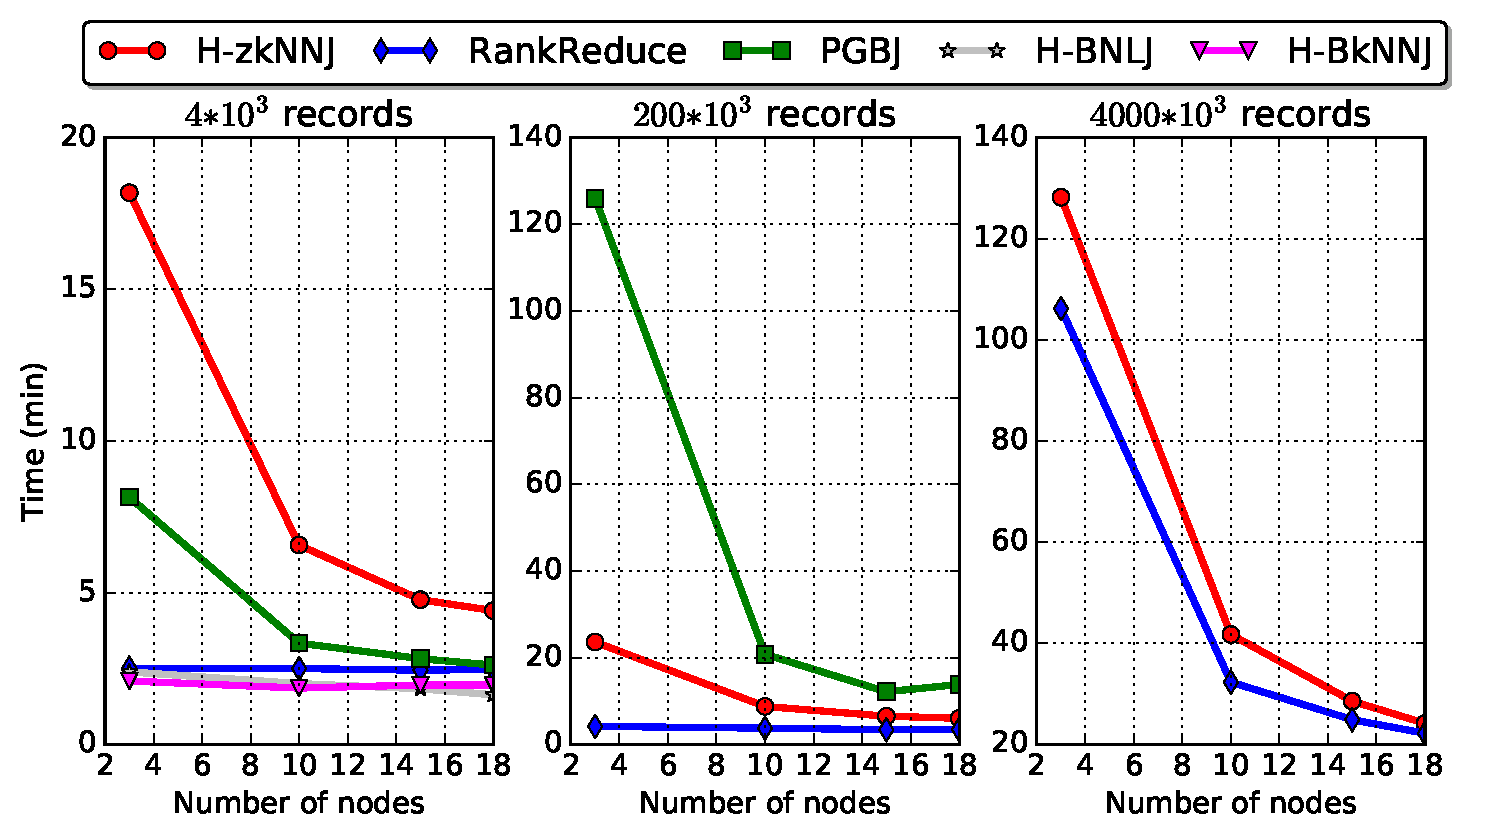
\includegraphics[width=0.5\textwidth]{img-perf/geo/data/nodes.pdf}
 \caption{Impact of the number of nodes on computing time  \label{fig:geo_data_nodes}}
\end{figure}
As expected, the computing time is strongly related to the number of nodes. Adding more nodes increases parallelism, reducing the
overall computing time. There is however a significant slow down after using more than 15 machines. Based on those
results, and considering the fact that we later use larger datasets, we conducted all subsequent experiments using at 
most 20 nodes.


\subsection{Geographic dataset}
\label{section:geo_dataset}

%%%% generated by 2-time.py
\begin{figure*}[htp]
	\centering
	\begin{subfigure}[b]{0.35\textwidth}
		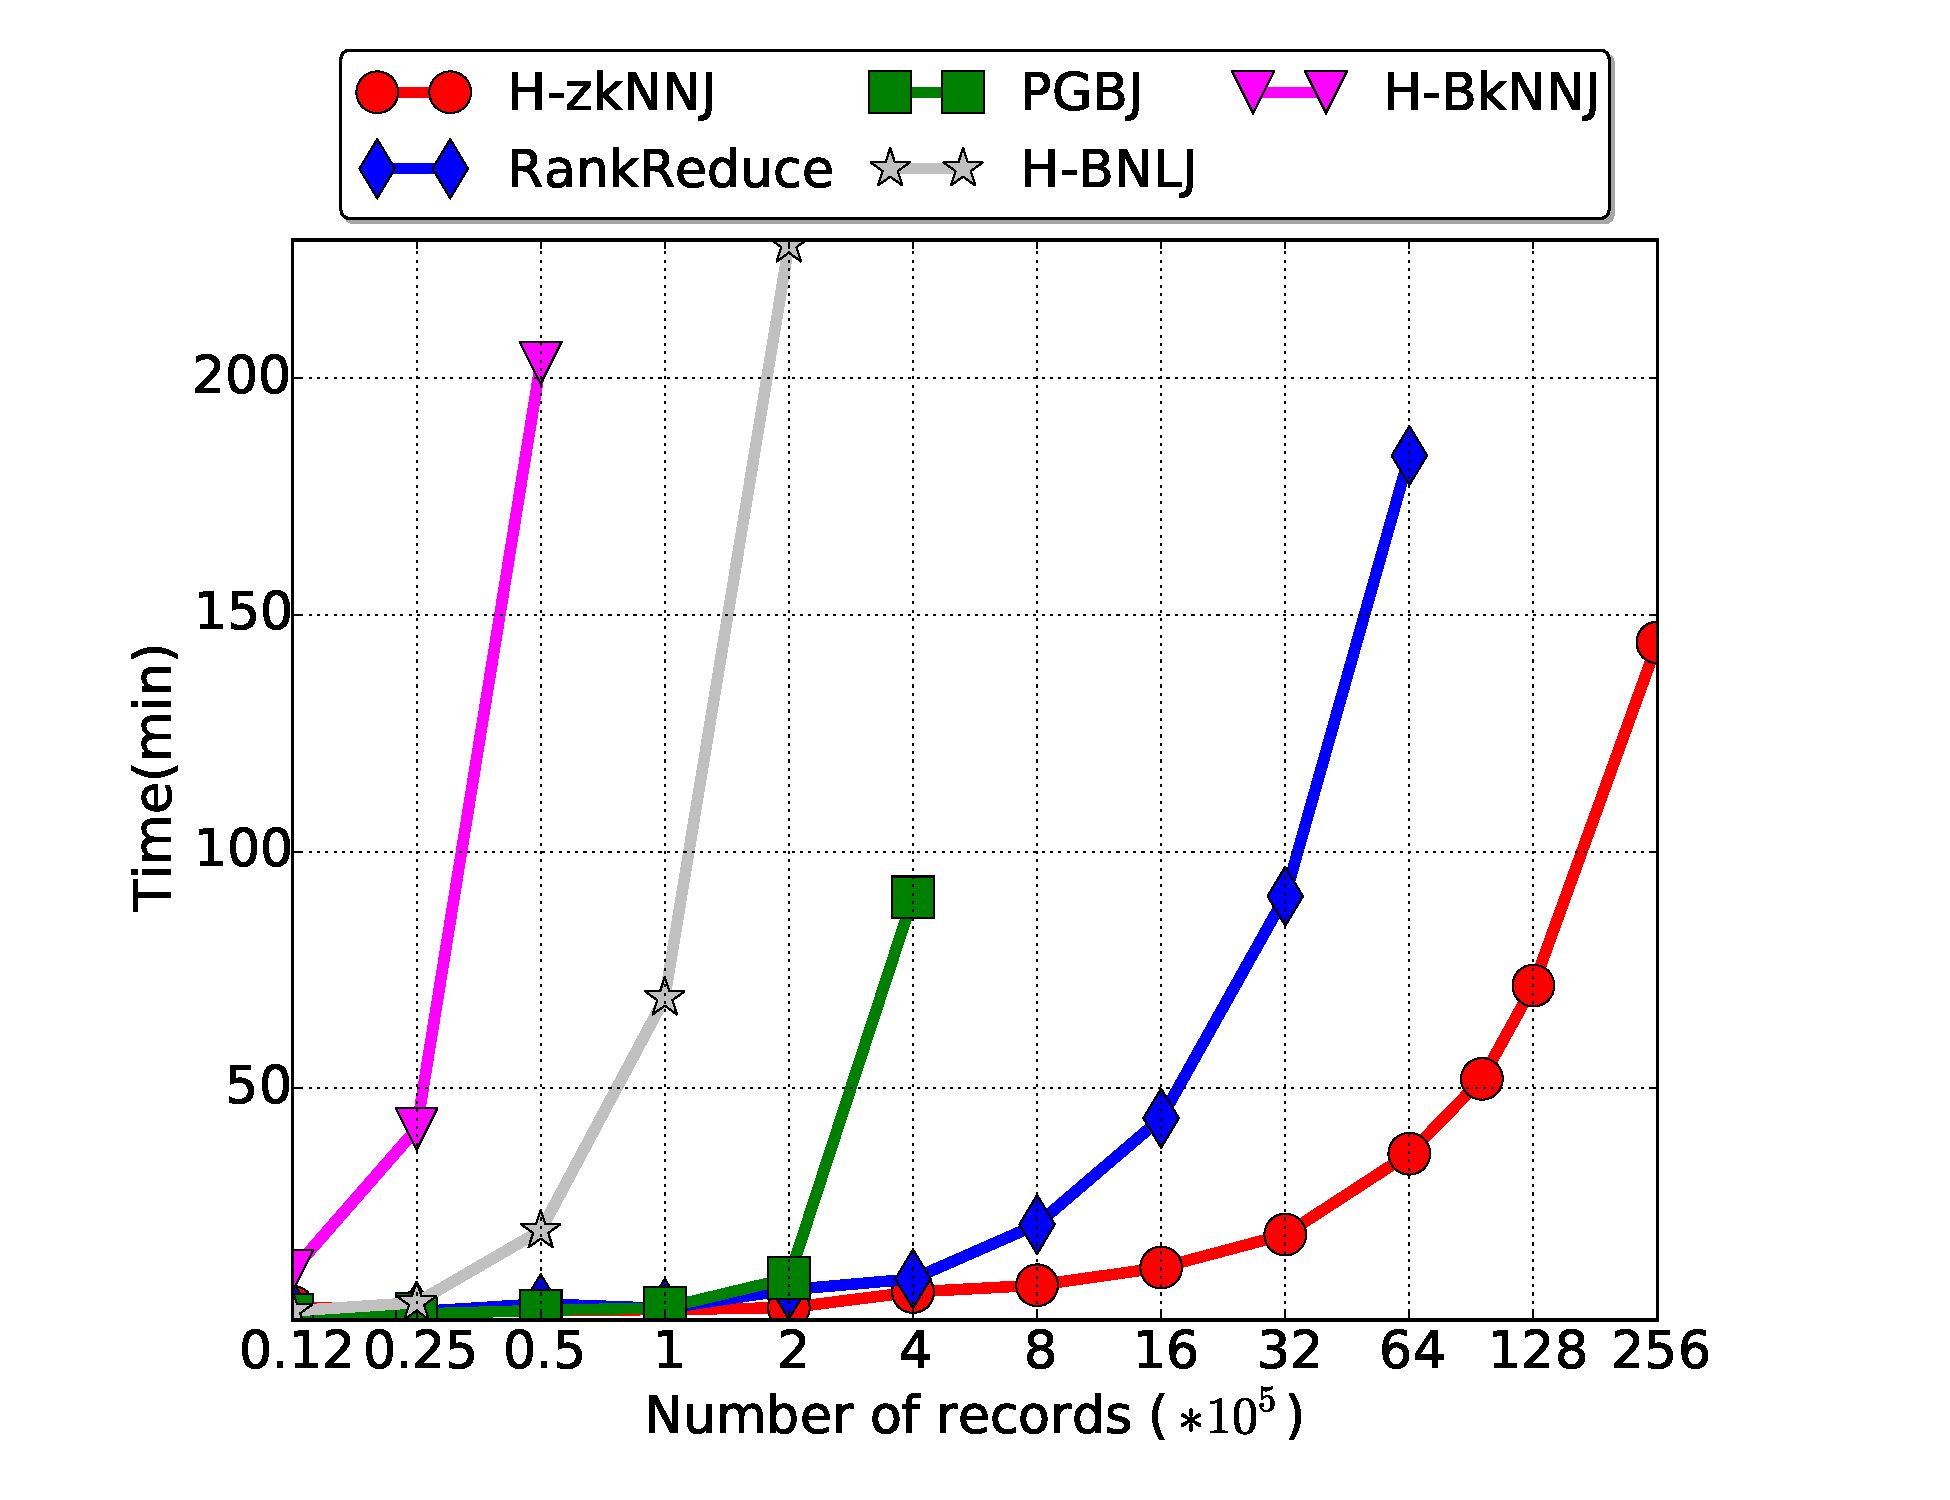
\includegraphics[width=\textwidth]{img-perf/geo/data/time.pdf} 
		\caption{Time}
		\label{fig:geo_data_time}
	\end{subfigure}%
	\begin{subfigure}[b]{0.35\textwidth}
		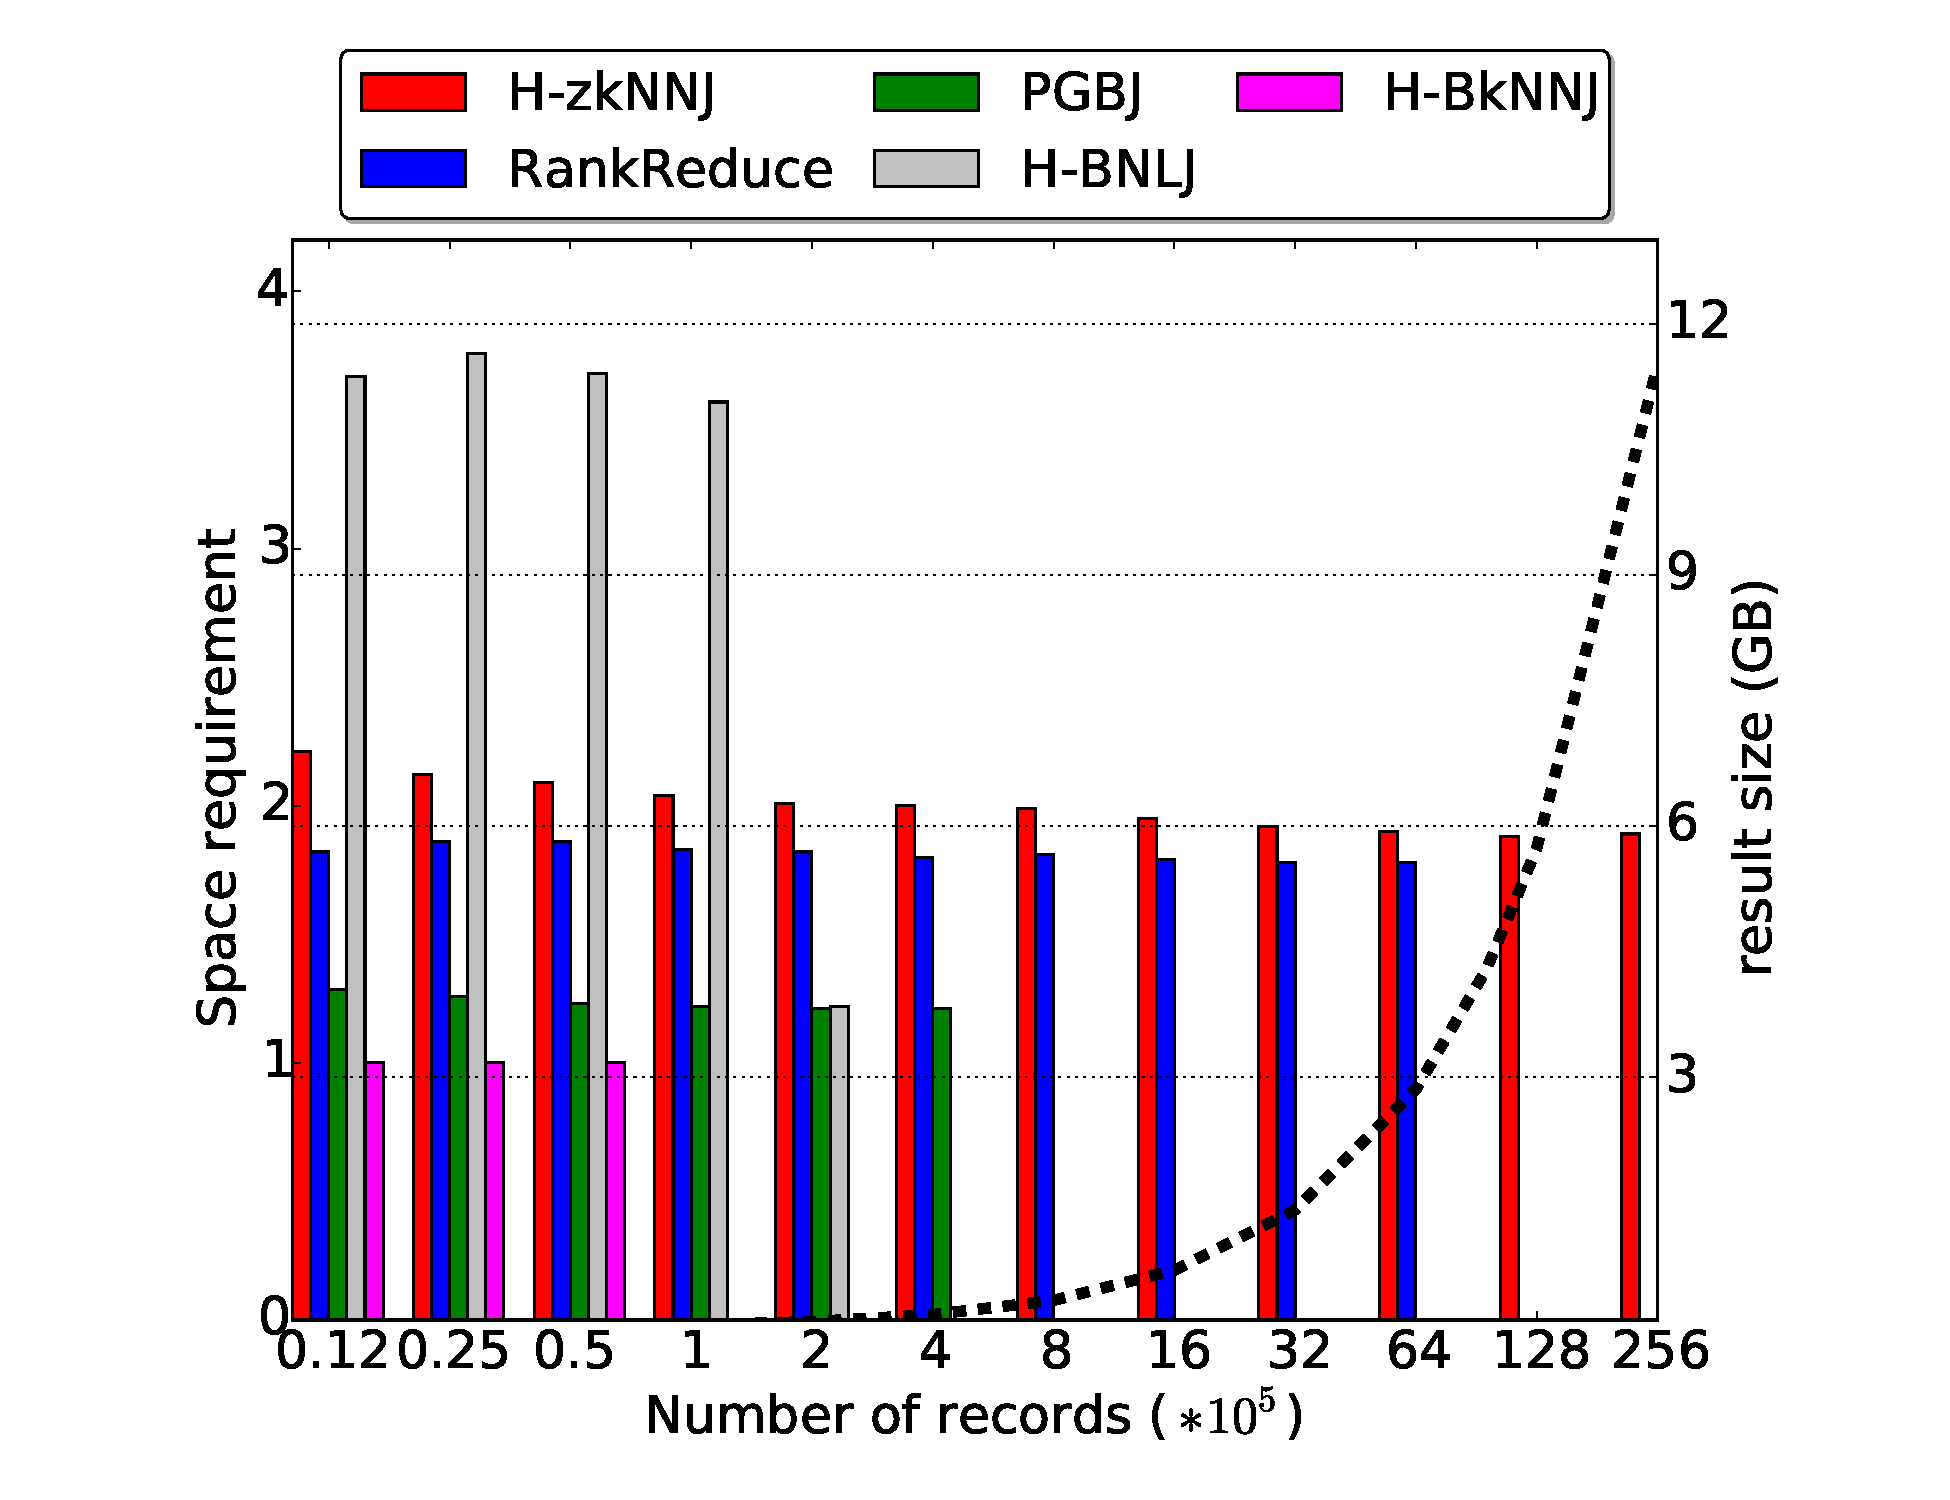
\includegraphics[width=\textwidth]{img-perf/geo/data/memory.pdf} 
		\caption{Result size and Disk Usage}
		\label{fig:geo_data_memory}
	\end{subfigure}%
	\begin{subfigure}[b]{0.35\textwidth}
		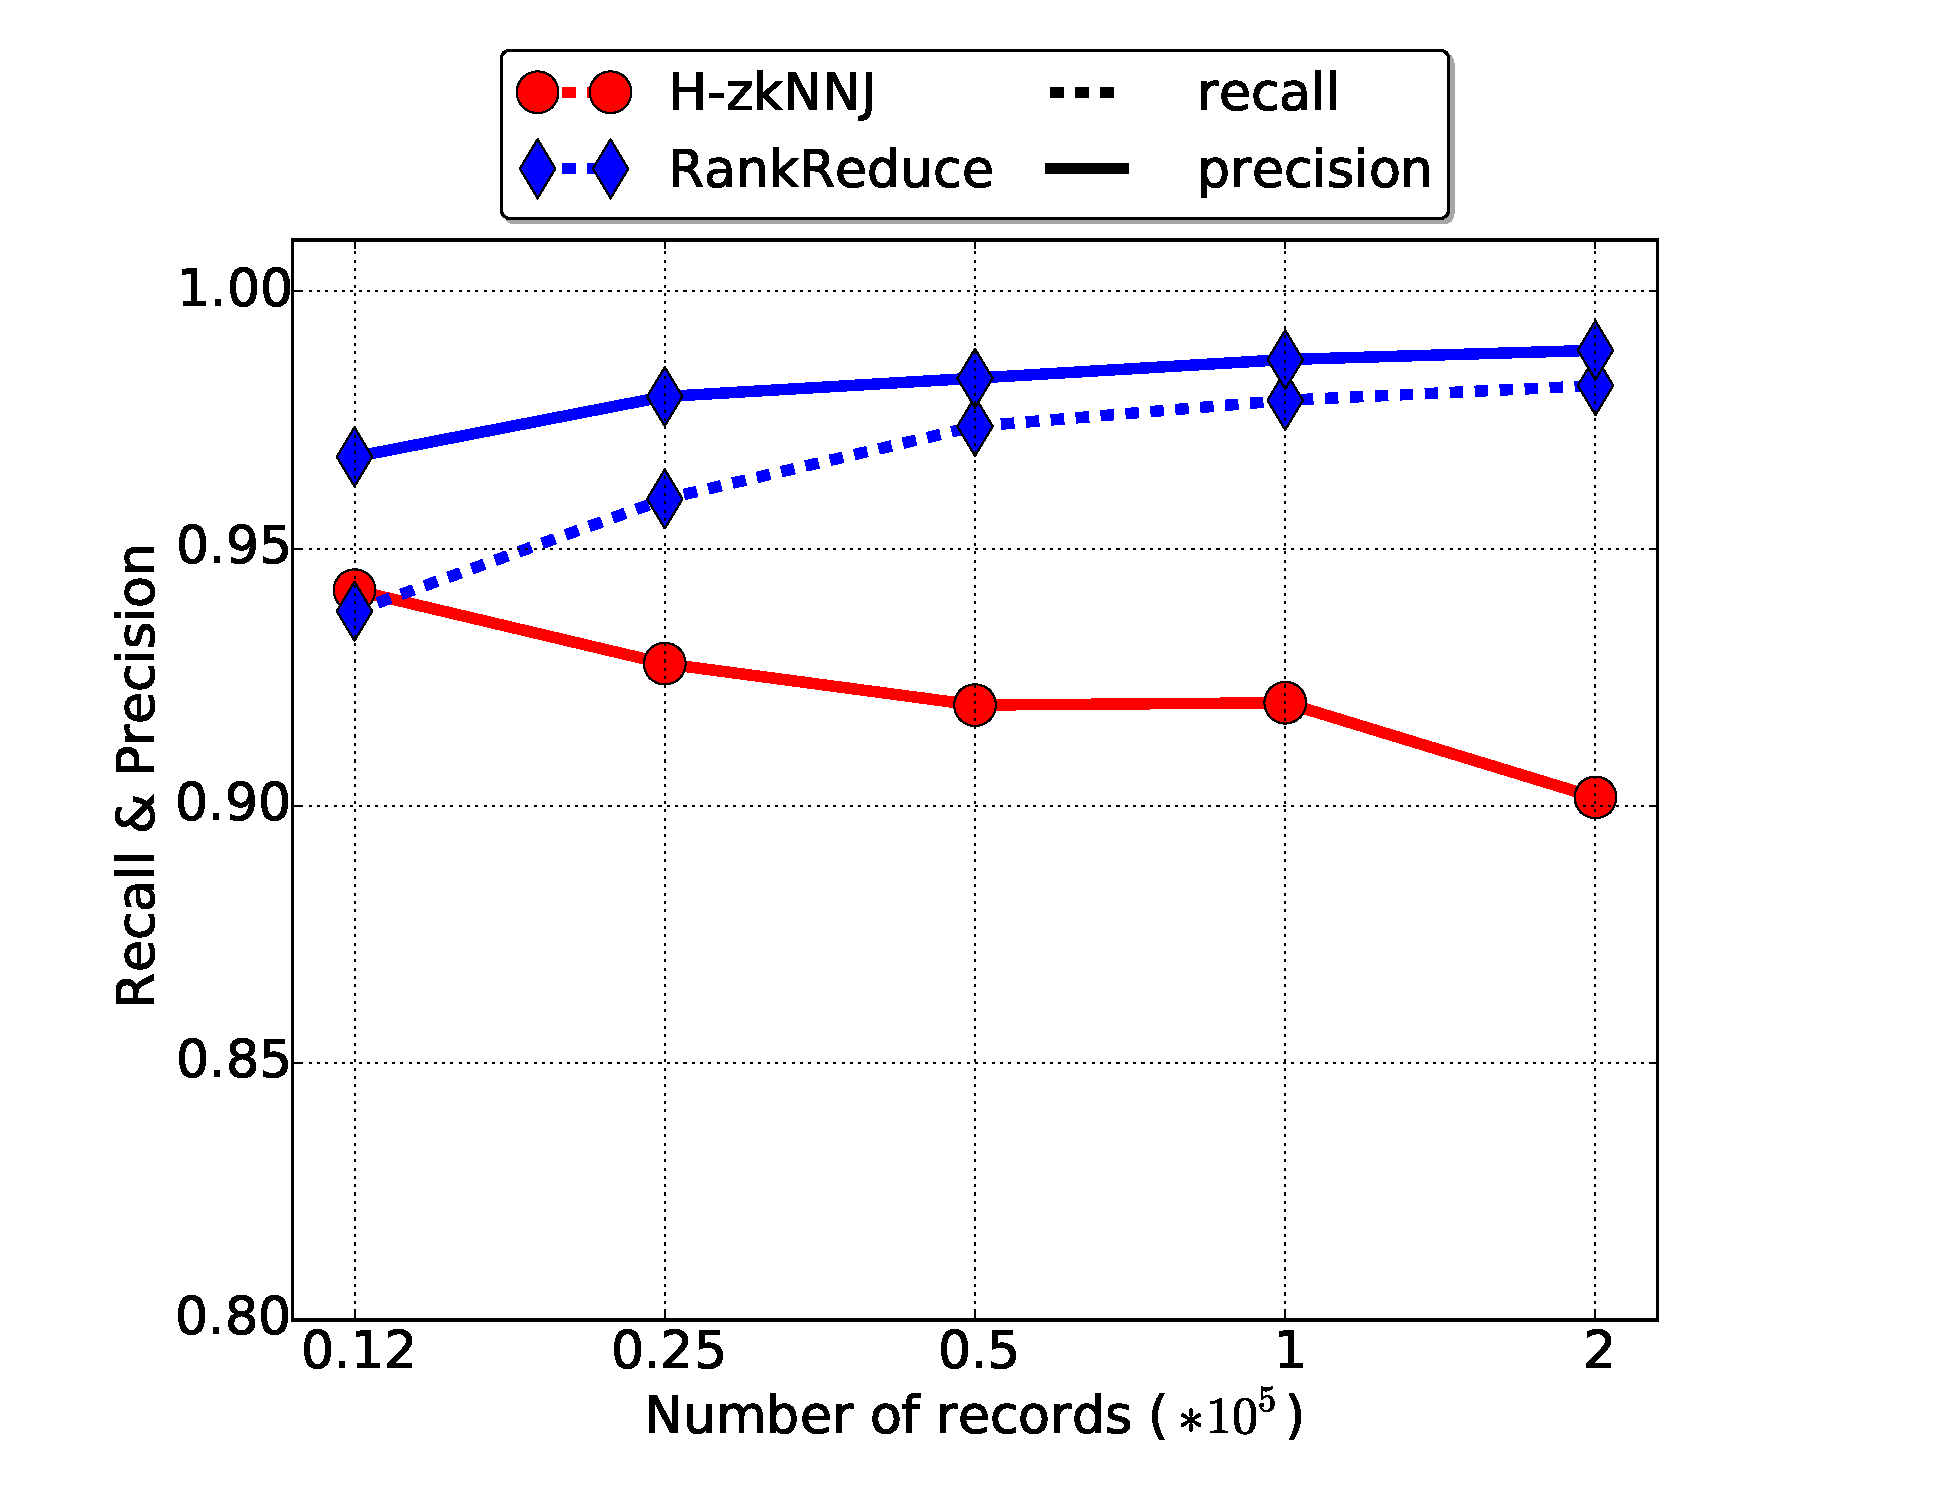
\includegraphics[width=\textwidth]{img-perf/geo/data/accuracy.pdf} 
		\caption{Recall and Precision \label{fig:geo_data_acc}}
	\end{subfigure}%
	\caption{Geo dataset impact of the data set size \label{geo_dataset}}
\end{figure*}


For all experiments in this section, we used the parameters described in Table~\ref{table:parameters_geo}.
Details regarding each parameter can be found in sections \ref{data_preprocessing} and  \ref{partitioning}. For 
RankReduce, the value of $W$ was adapted to get the best performance from each dataset. For datasets up to $16*10^5$
records, $W=32*10^{5}$, up to $25*10^{5}$ records, $W=25*10^{5}$ and finally, $W=15*10^{5}$ for the rest of the 
experiments. 

% shown in Table~\ref{table:parameters_geo}.
\begin{table}[ht]
\begin{center}{\renewcommand{\arraystretch}{1.2} % to prevent equation from being chopped 
\begin{tabular}{|c|c|c|c|}
\hline
\textbf{Algorithm} & \textbf{Partitioning} & \textbf{Reducers} & \textbf{Configuration}  \\ \hline
\HBNLJ             & 10 partitions  & 100 reducers & \\ \hline
\VO               & 3000 pivots     & 25 reducers       & \begin{tabular}[c]{@{}c@{}}k-means \\ + greedy\end{tabular} 
\\ \hline
\LSH          & $W = \left\{
\begin{array}{l}  
	32*10^{5}\\    
    25*10^{5}\\
	15*10^{5}\\
\end{array}\right.$
%$32*10^{5}$
% \TODO{this is plustot the size of bucket but not the number of partition. ??}           
& 25 reducers       & \begin{tabular}[c]{@{}c@{}}L = 2\\ M = 7\end{tabular}       \\ \hline
\Z~           & 10 partitions         & 30 reducers       & 3 shifts, 
p=10                                                     \\ \hline
\end{tabular}
}
\caption{Algorithm parameters \label{table:parameters_geo} for geographic dataset}
\end{center}
\end{table}


\subsubsection{Impact of input data size}
Our first set of experiments measures the impact of the data size on execution time, disk space and recall. 
Figure~\ref{fig:geo_data_time} shows the global computing time of all algorithms, varying 
the number of records from $0.125 * 10^{5}$ to $256 * 10^{5}$. The global computing time increases more or less 
exponentially for all algorithms, but only \Z~and \LSH~can process medium to large datasets. For 
small datasets, \VO~can compute an exact solution as fast as the other algorithms. 


Figure~\ref{fig:geo_data_memory} shows the space requirement of each algorithm as a function of the final output size. 
To 
reduce the footprint of each run, intermediate data are compressed. For example, for 
\HBNLJ, the size of intermediate data is $2.6$ times bigger than the size of output data. Overall, the algorithms with 
the
lowest space requirements are \LSH~and \VO.

Figure~\ref{fig:geo_data_acc} shows the recall and precision of the two approximate algorithms, \Z~and \LSH. Since \Z~
always return $k$ elements, its precision and recall are identical. 
As the number of records increases, its recall decreases, while still being high, because of the 
space filling curves used in the preprocessing phase.
On the other hand, the recall of \LSH~is always lower than its precision because it outputs less than $k$ elements. It
benefits from larger datasets because more data end up in the same bucket, increasing the 
number of candidates. Overall, the quality of \LSH~was found to be better than \Z~on the Geo dataset. 

%\input{parts/exp-dim-figure.tex}
\subsubsection{Impact of k}
Changing the value of $k$ can have a significant impact on the performance of some of the kNN 
algorithms. We experimented on a dataset of $2*10^5$ records (only $5*10^4$ for \HBNLJ~ 
for performance reasons) with values for $k$ varying from 2 to 512. Results are shown in 
Figure~\ref{fig:geo_impact_k} using a logarithmic scale on the x-axis.

First, we observe a global increase in computing time (Figure~\ref{fig:geo_k_time}) which matches the complexity 
analysis performed earlier. 
As $k$ increases, the performance of \Z, compared to the other advanced algorithms, decreases. This is due to the 
necessary replication of the $z$-values of $S$ throughout the partitions to find enough candidates: the core 
computation is thus much more complex. 

%%% generated by A4-ratioByK.py
\begin{figure*}[htp]
	\centering
	\begin{subfigure}[b]{0.35\textwidth}
		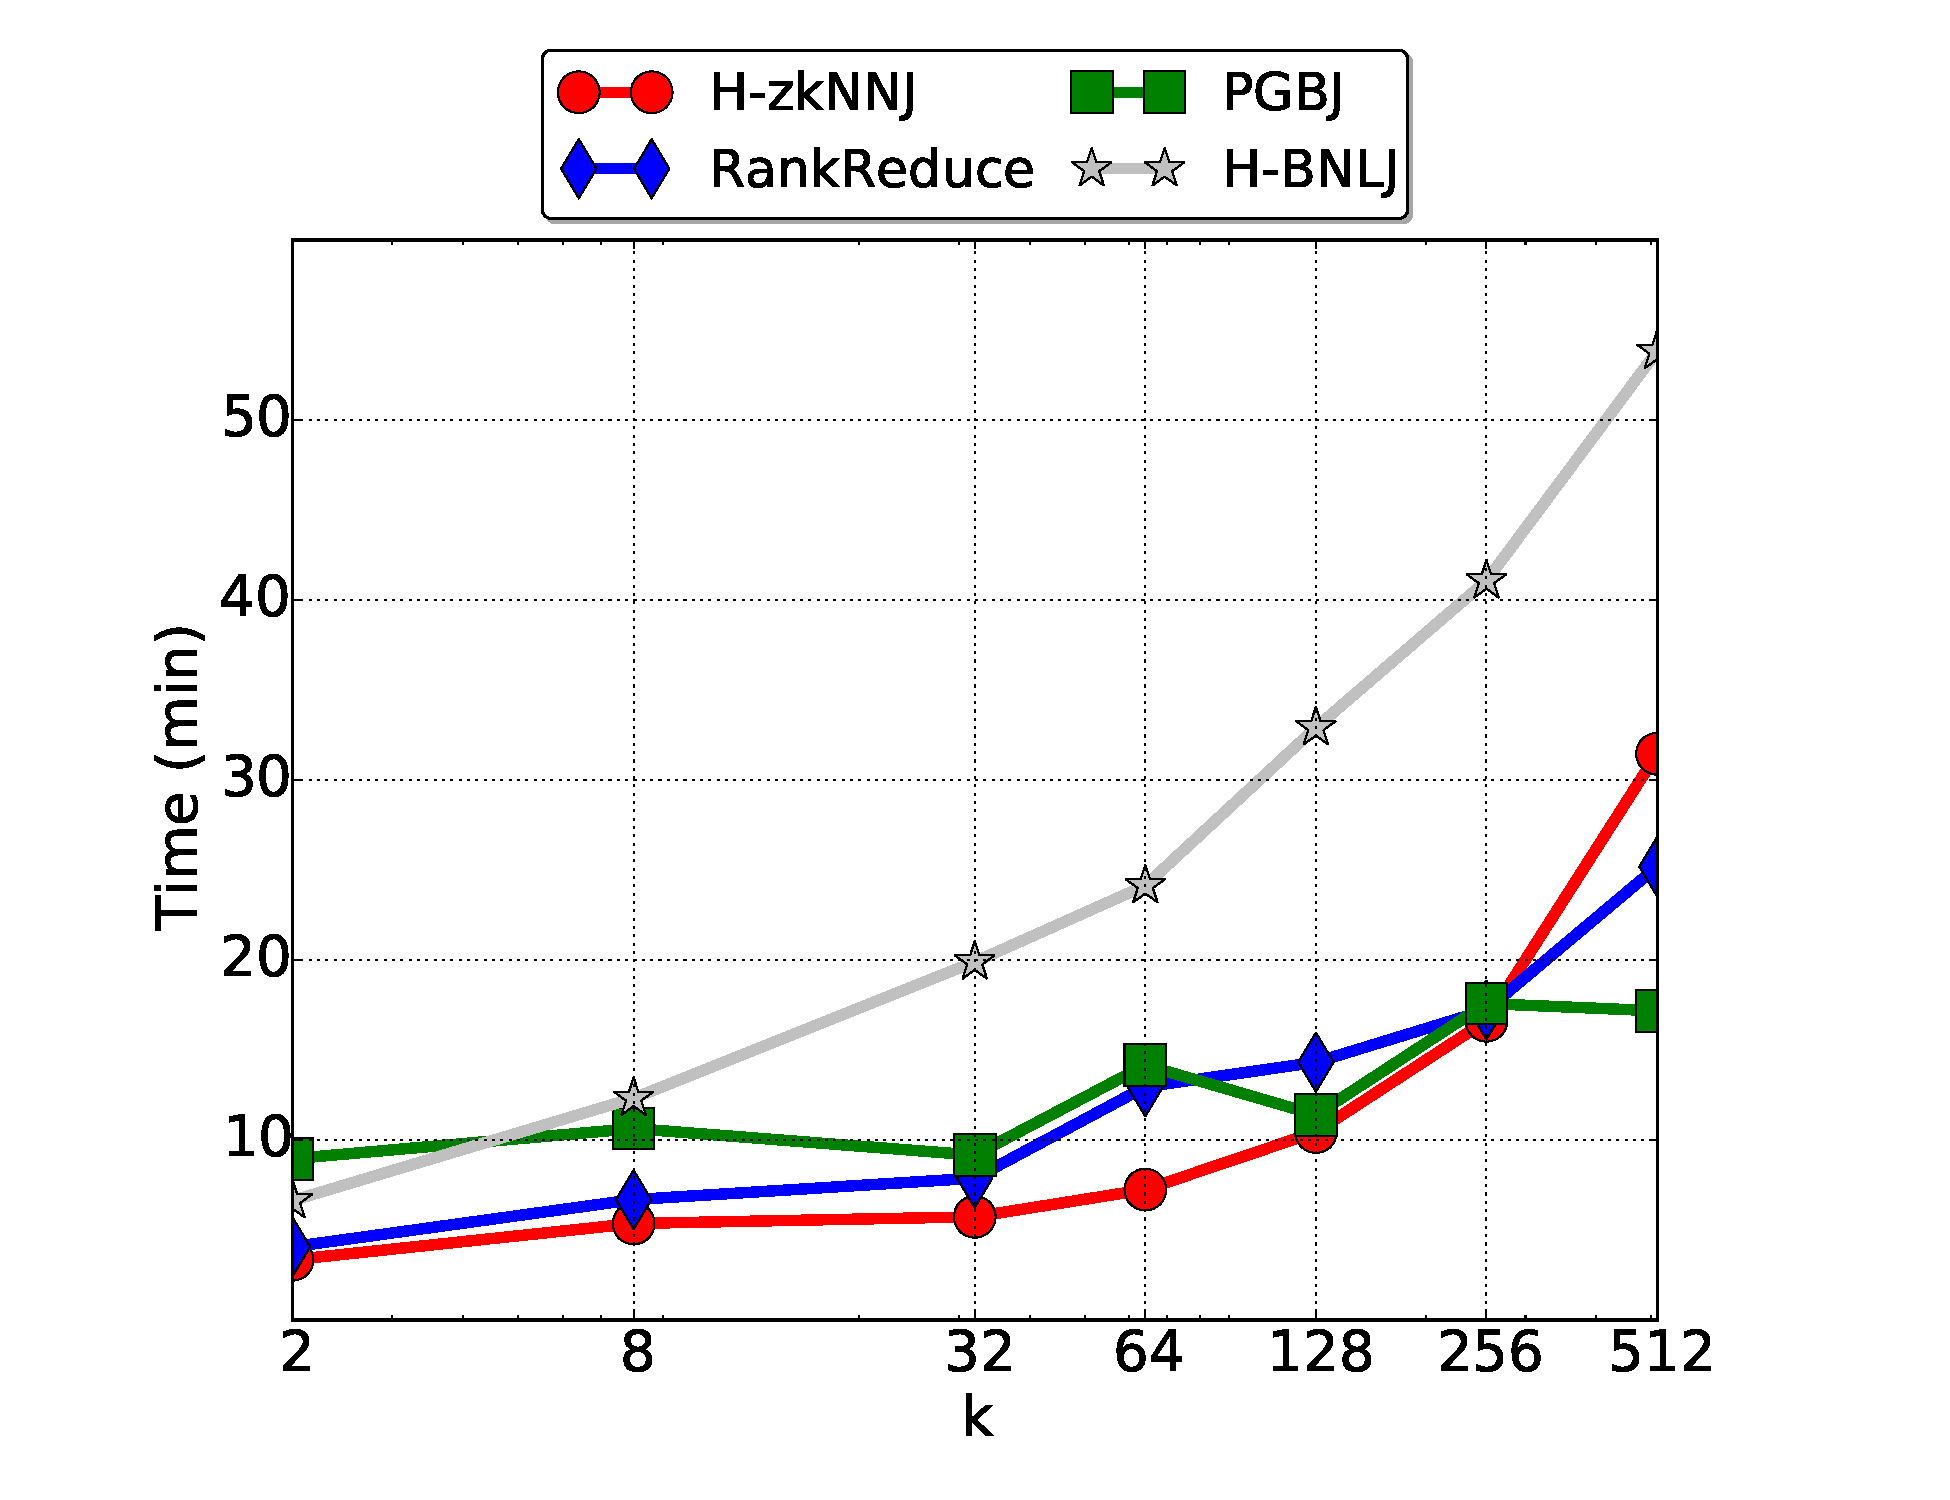
\includegraphics[width=\textwidth]{img-perf/geo/k/time.pdf} 
		\caption{Time\label{fig:geo_k_time}}       
	\end{subfigure}%
	\begin{subfigure}[b]{0.35\textwidth}
		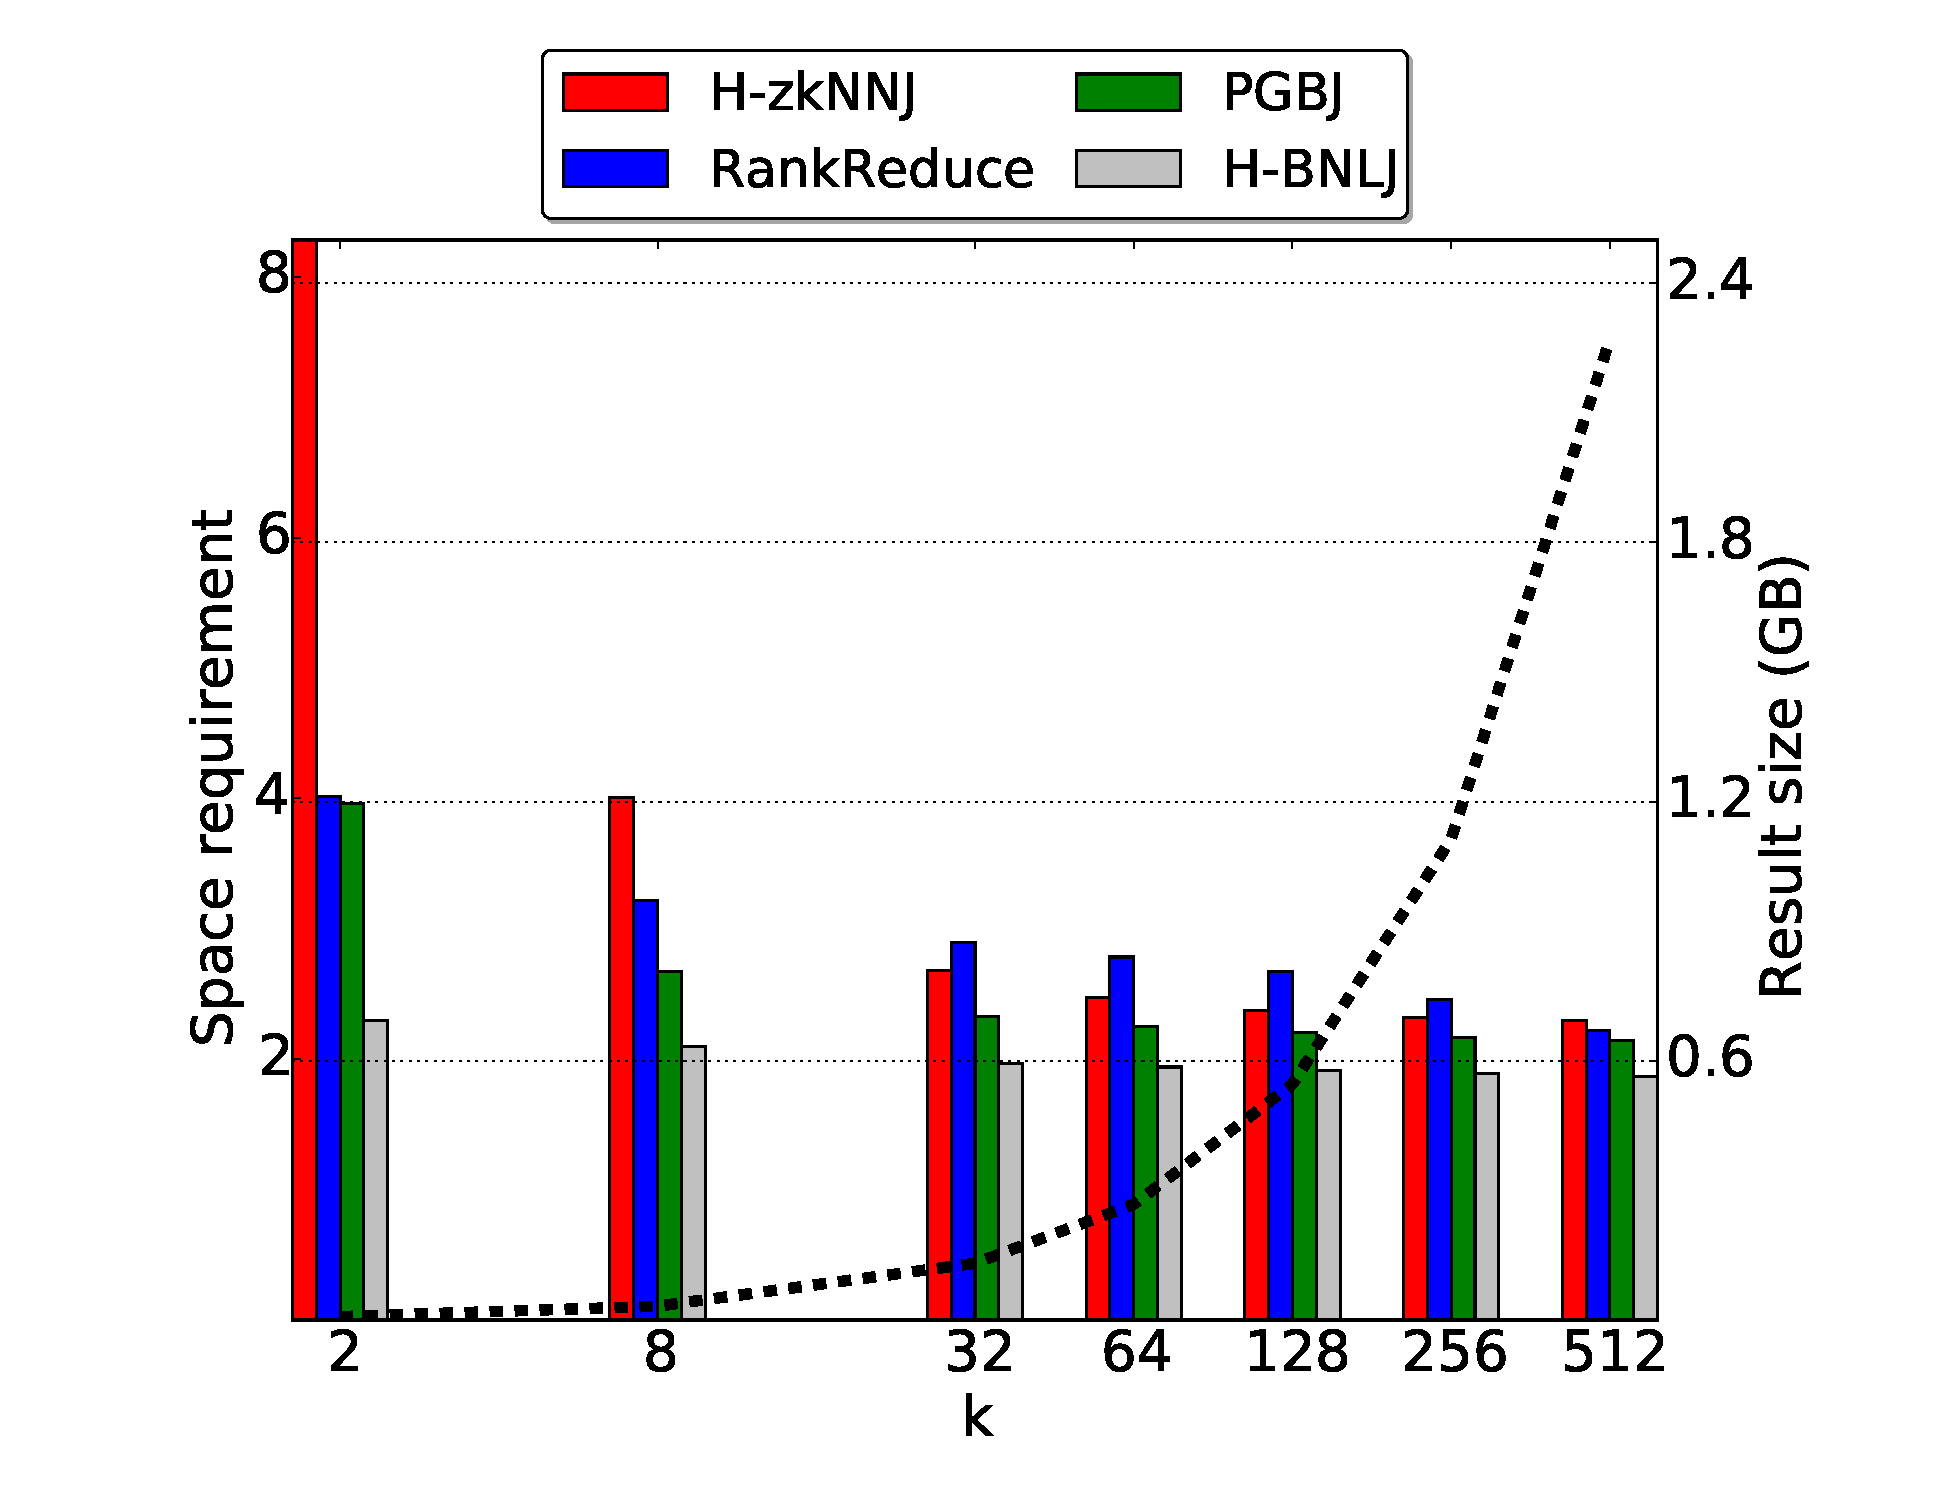
\includegraphics[width=\textwidth]{img-perf/geo/k/memory.pdf} 
		\caption{Result size and Disk Usage\label{fig:geo_k_memory} }
	\end{subfigure}%
	\begin{subfigure}[b]{0.35\textwidth}
		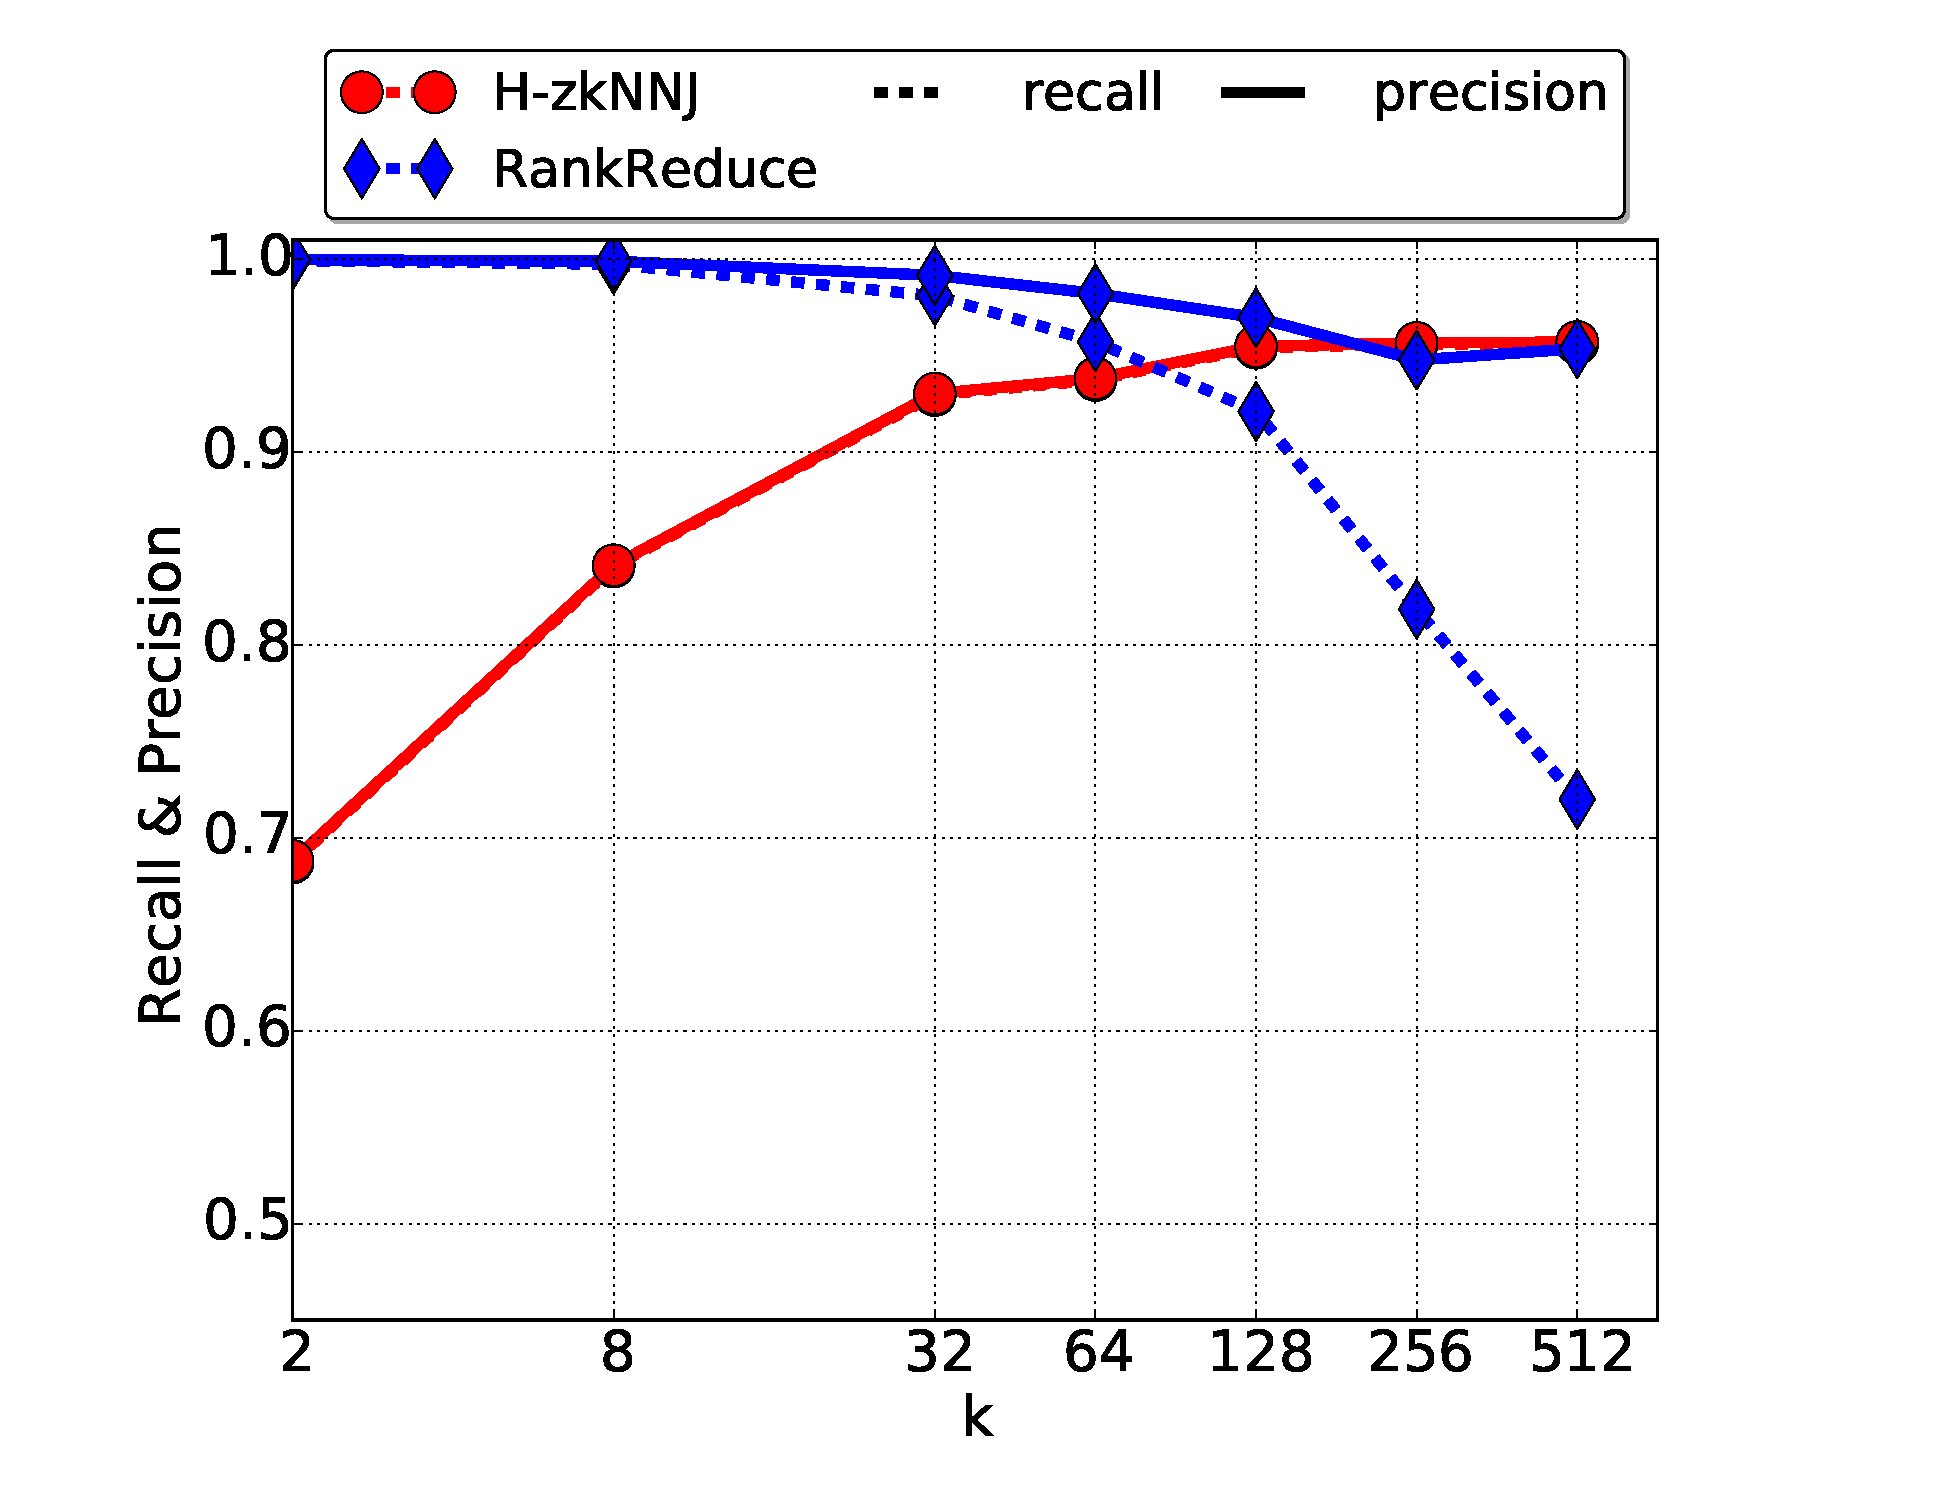
\includegraphics[width=\textwidth]{img-perf/geo/k/accuracy.pdf} 
		\caption{Recall and Precision \label{fig:geo_k_acc}}            
	\end{subfigure}%
	\caption{ Geo dataset with 200k records (50k for H-BNLJ), impact of $K$  }
	\label{fig:geo_impact_k}
\end{figure*}

Second, the algorithms can also be distinguished considering their disk usage, visible on 
Figure ~\ref{fig:geo_k_memory}. The global tendency is that the ratio of intermediate data size over the final data 
size decreases. This means that for each algorithm the final 
data size grows faster than the intermediate data size. As a consequence, there is no particular algorithm that 
suffers from such a bottleneck at this point.
\VO~is \ the most efficient from this aspect. Its replication of data occurs independently of the number of 
selected neighbors. Thus, increasing $k$ has a small impact on this algorithm, both in computing time and space 
requirements. On this figure, an interesting observation can also be made for \Z. For $k=2$, it has by far the 
largest disk
usage but becomes similar to the others for larger values. 
This is because \Z~creates a lot of intermediate data (copies of the initial dataset, vectors for the space 
filling curve, sampling...) irrespective of the value of $k$. As $k$ increases, so does the output size, mitigating the 
impact of these intermediate data. 

Surprisingly, changing $k$ has a different impact on the recall of the approximate kNN methods, as can be seen on 
Figure~\ref{fig:geo_k_acc}.
For \LSH, increasing $k$ has a negative impact on the recall which sharply decreases when $k\geq 64$. This is
because the window parameter ($W$) of LSH was set at the beginning of the experiments to achieve the best performance for this
particular dataset. However, it was not modified for various of $k$. Thus it became less optimal as $k$ increased. This 
shows there is a link between global parameters such 
as $k$ and parameters of the LSH process. When using \Z, 
increasing $k$  improves the precision: the probability to have incorrect points is reduced as there are more 
candidates in a single partition. 

\subsubsection{Communication Overhead}
Our last set of experiments looks at inter-node communication by measuring the amount of data transmitted during the
shuffle phase (Figure~\ref{fig:geo_communication}). The goal is to compare these measurements with the theoretical 
analysis in Section~\ref{section:global_complexity}, 

%%%% Generated with   2-time.py  and A4-ratioByK.py
\begin{figure*}[htp]
	\centering
	\begin{subfigure}[b]{0.48\textwidth}
		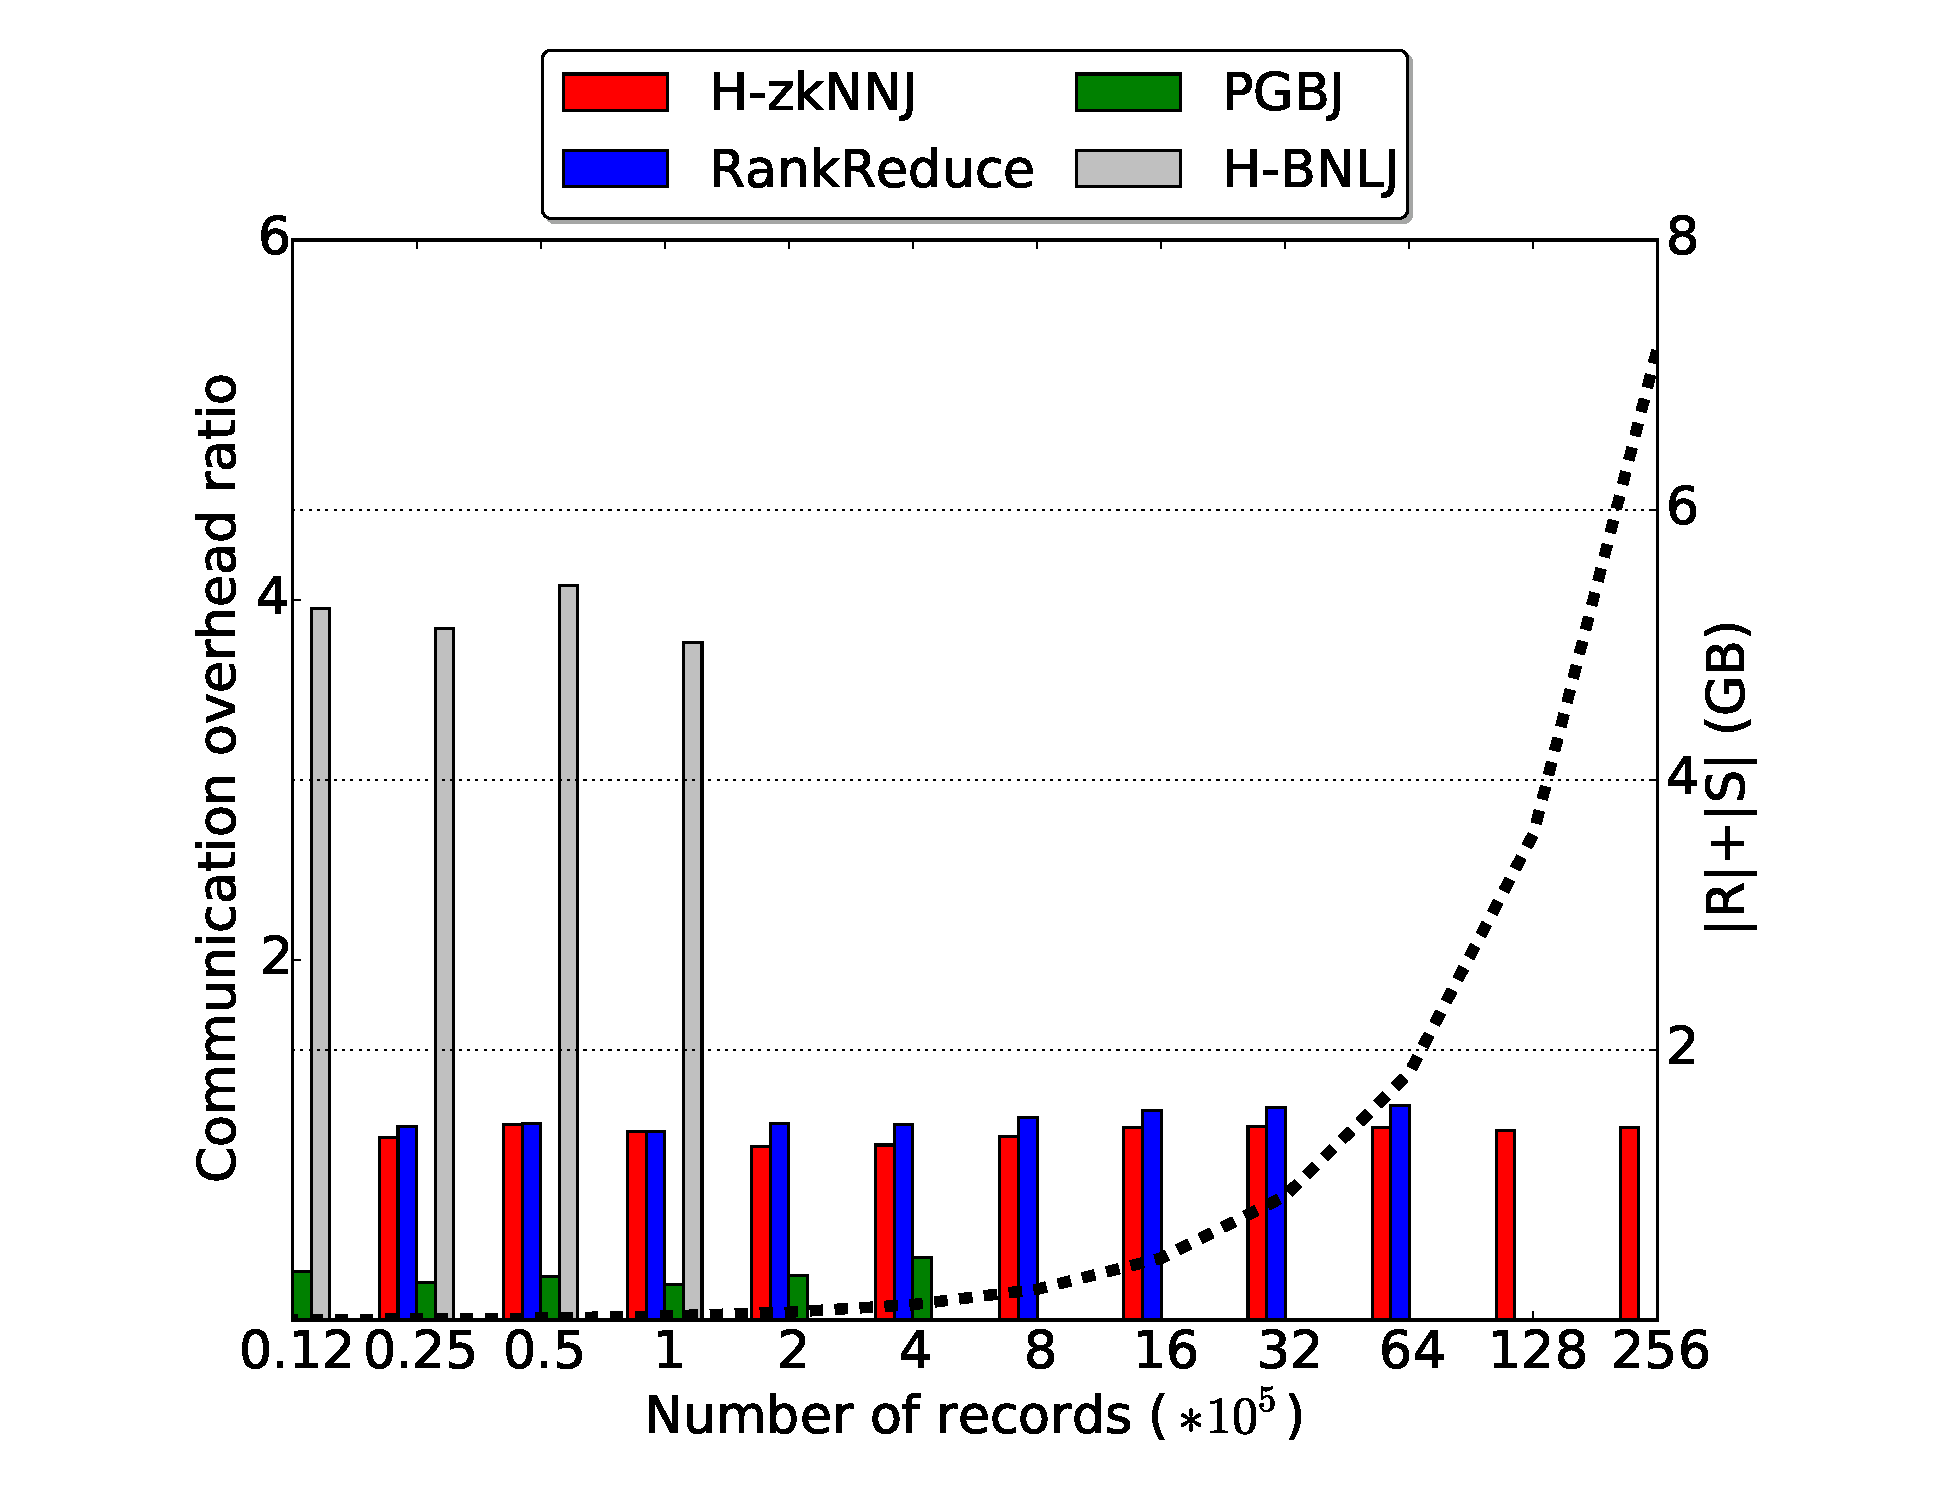
\includegraphics[width=\textwidth]{img-perf/geo/data/shuffle.pdf} 
		\caption{Impact of the data set size\label{fig:geo_data_shuffle}}
	\end{subfigure}%
	\begin{subfigure}[b]{0.48\textwidth}
		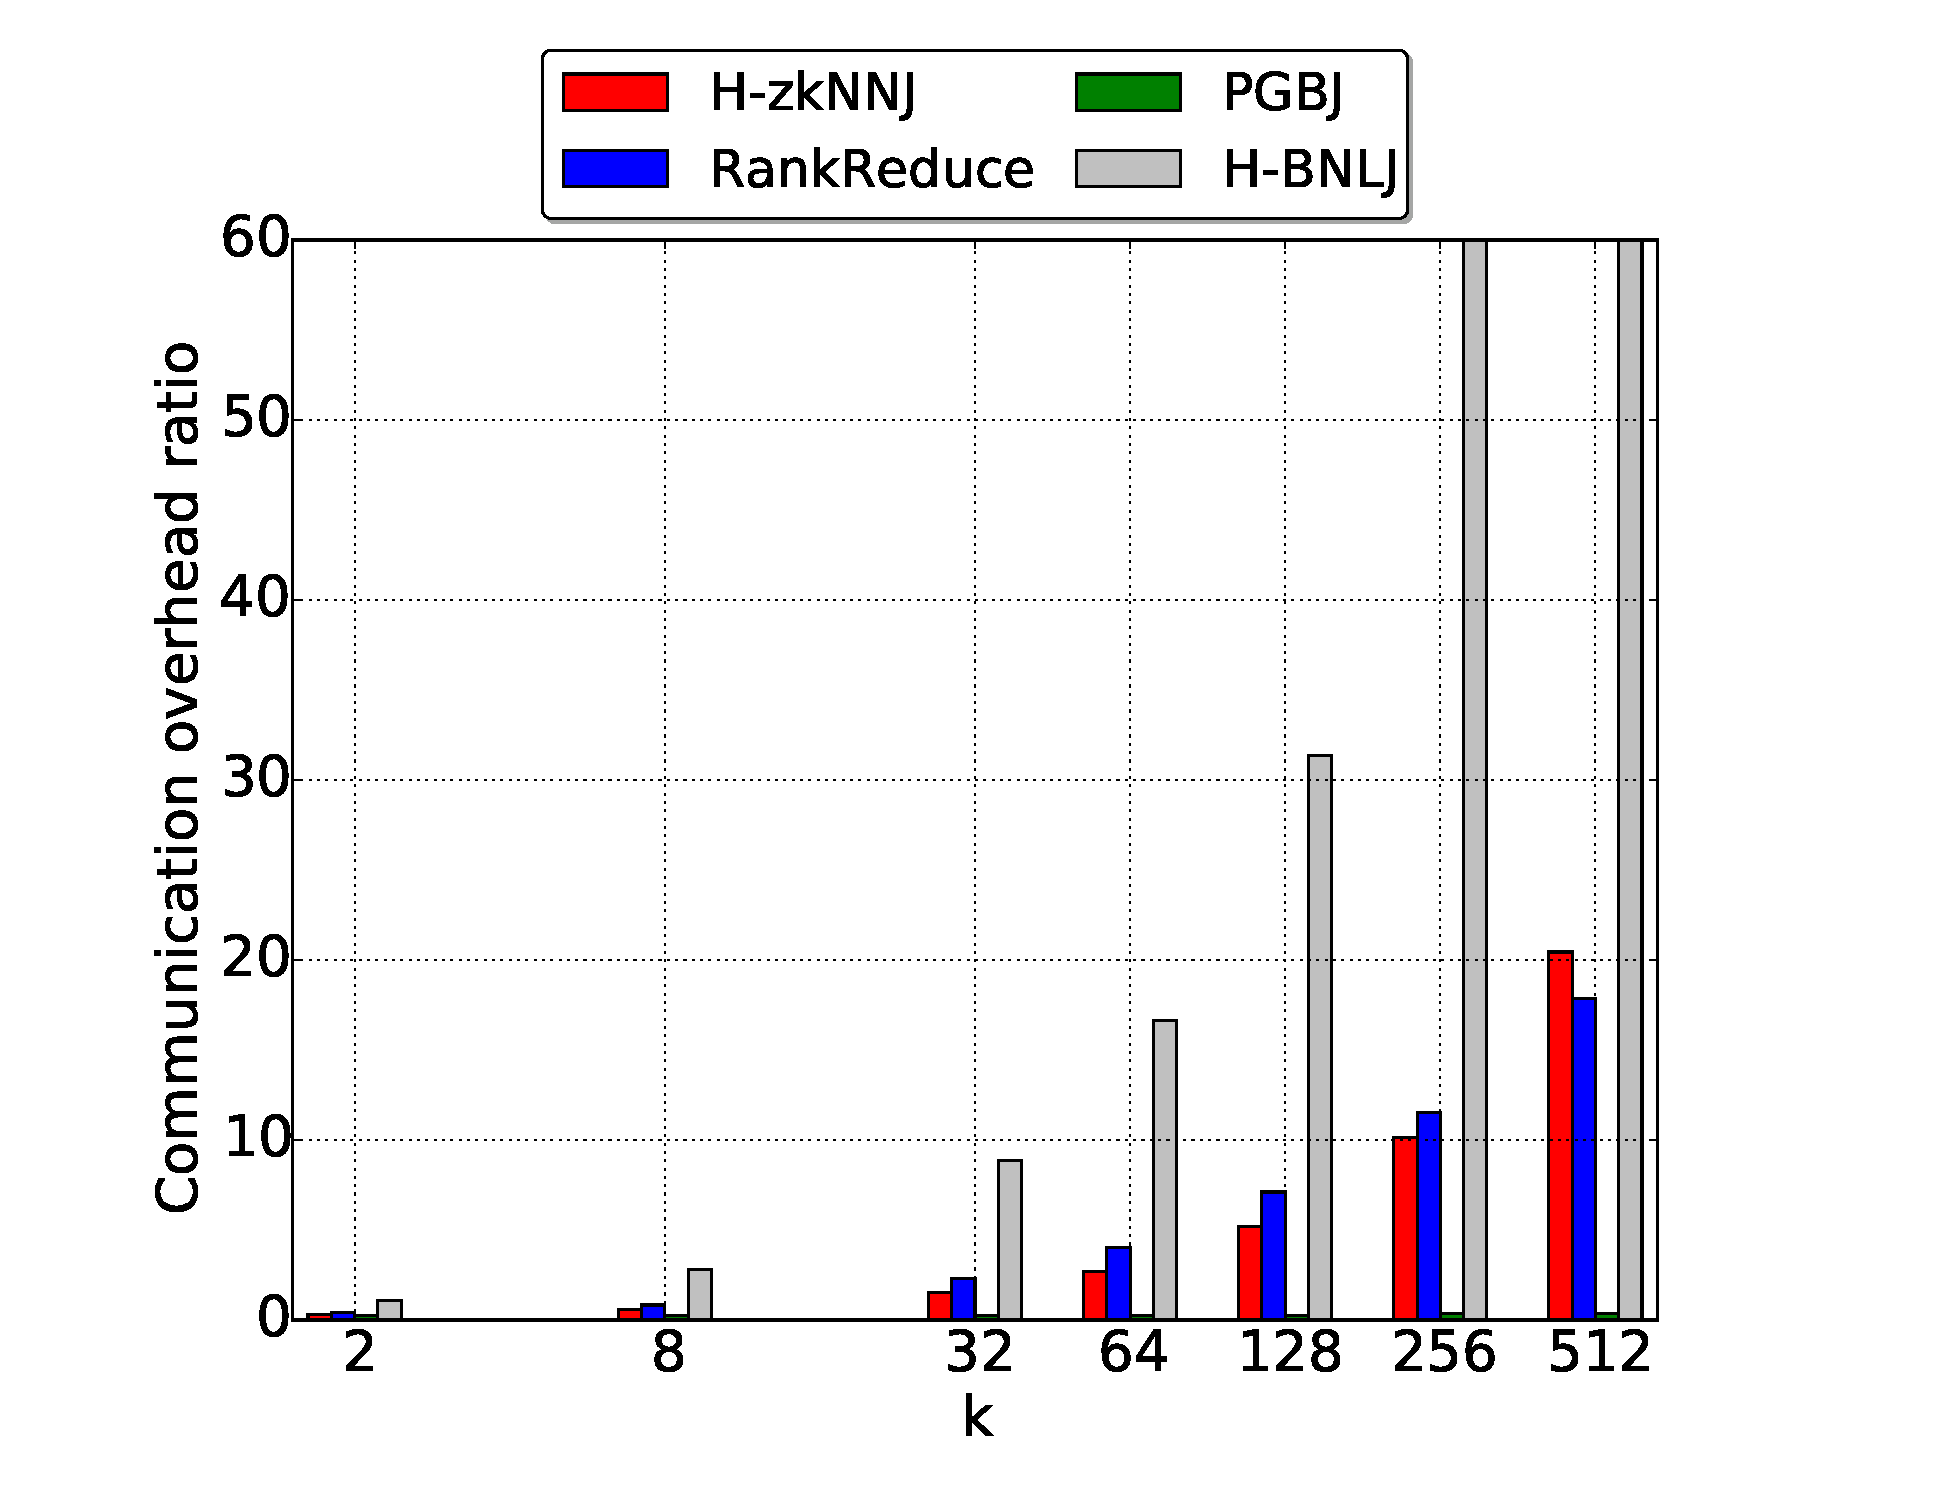
\includegraphics[width=\textwidth]{img-perf/geo/k/shuffle.pdf} 
		\caption{Impact of $K$ with $2*10^5$ records ($0.5*10^5$ for H-BNLJ) \label{fig:geo_k_shuffle}}
	\end{subfigure}%
	\caption{Geo dataset, communication overhead \label{fig:geo_communication}}      
\end{figure*}

\emph{Impact of data size.} For Geo dataset (Figure~\ref{fig:geo_data_shuffle}), \HBNLJ~has indeed a lot of 
communication. For a dataset of $1*10^5$ records, the shuffle phase transmits almost $4$ times the original size.
Both \LSH~and \Z~have a constant factor of $1$ because of the duplication of the original 
dataset
to improve the recall. The most efficient algorithm is \VO~for two reasons. First it does not duplicate the 
original dataset and second, it relies on various grouping strategies to minimize replication.

\emph{Impact of k.}
We have performed another set of experiments, with a fixed dataset of $2*10^5$ records (only $0.5*10^5$ for \HBNLJ). 
The results can be seen in Figure~\ref{fig:geo_k_shuffle}. For different values of $k$, we have a similar hierarchy 
than with the data size. For \LSH~and \Z, the shuffle increases linearly because the number of candidates in the second 
phase depends on $k$. Moreover \Z~also replicates $k$ previous and succeeding elements in the first phase, and because 
of that, its overhead becomes significant for large $k$. Finally in \VO, $k$ has no impact on the shuffle phase.


\subsection{Image Feature Descriptors (SURF) dataset}
\label{section:surf_dataset}
We now investigate whether the dimension of input data has an impact on the kNN algorithms using the SURF dataset.
We used the Euclidian distance between descriptors to measure image similarity. 
For all experiments in this section, the parameters mentioned in Table~\ref{table:parameters} are used.
\begin{table}[h]
\begin{center}{\renewcommand{\arraystretch}{1.2}
\begin{tabular}{|c|c|c|c|}
\hline
\textbf{Algorithm} & \textbf{Partitioning} & \textbf{Reducers} & 
\textbf{Configuration}                                              \\ \hline
\HBNLJ            & 10 partitions         & 100 reducers      
&                                                             \\ \hline
\VO               & 3000 pivots           & 25 reducers       & \begin{tabular}[c]{@{}c@{}}k-means \\ + 
geo\end{tabular} \\ \hline
\LSH         & W = $10^7$     & 25 reducers       & \begin{tabular}[c]{@{}c@{}}L 
= 5\\ M = 7\end{tabular}       \\ \hline
\Z~           & 6 partitions         & 30 reducers       & 5 shifts                                                    
\\ \hline
\end{tabular}
}
\caption{Algorithm parameters \label{table:parameters} for SURF dataset}
\end{center}
\end{table}

%\input{parts/exp-surf-figure.tex}


%%%% Generated by B00-surf.py
\begin{figure*}[htp]
	\centering
	\begin{subfigure}[b]{0.35\textwidth}
		% \fbox{
		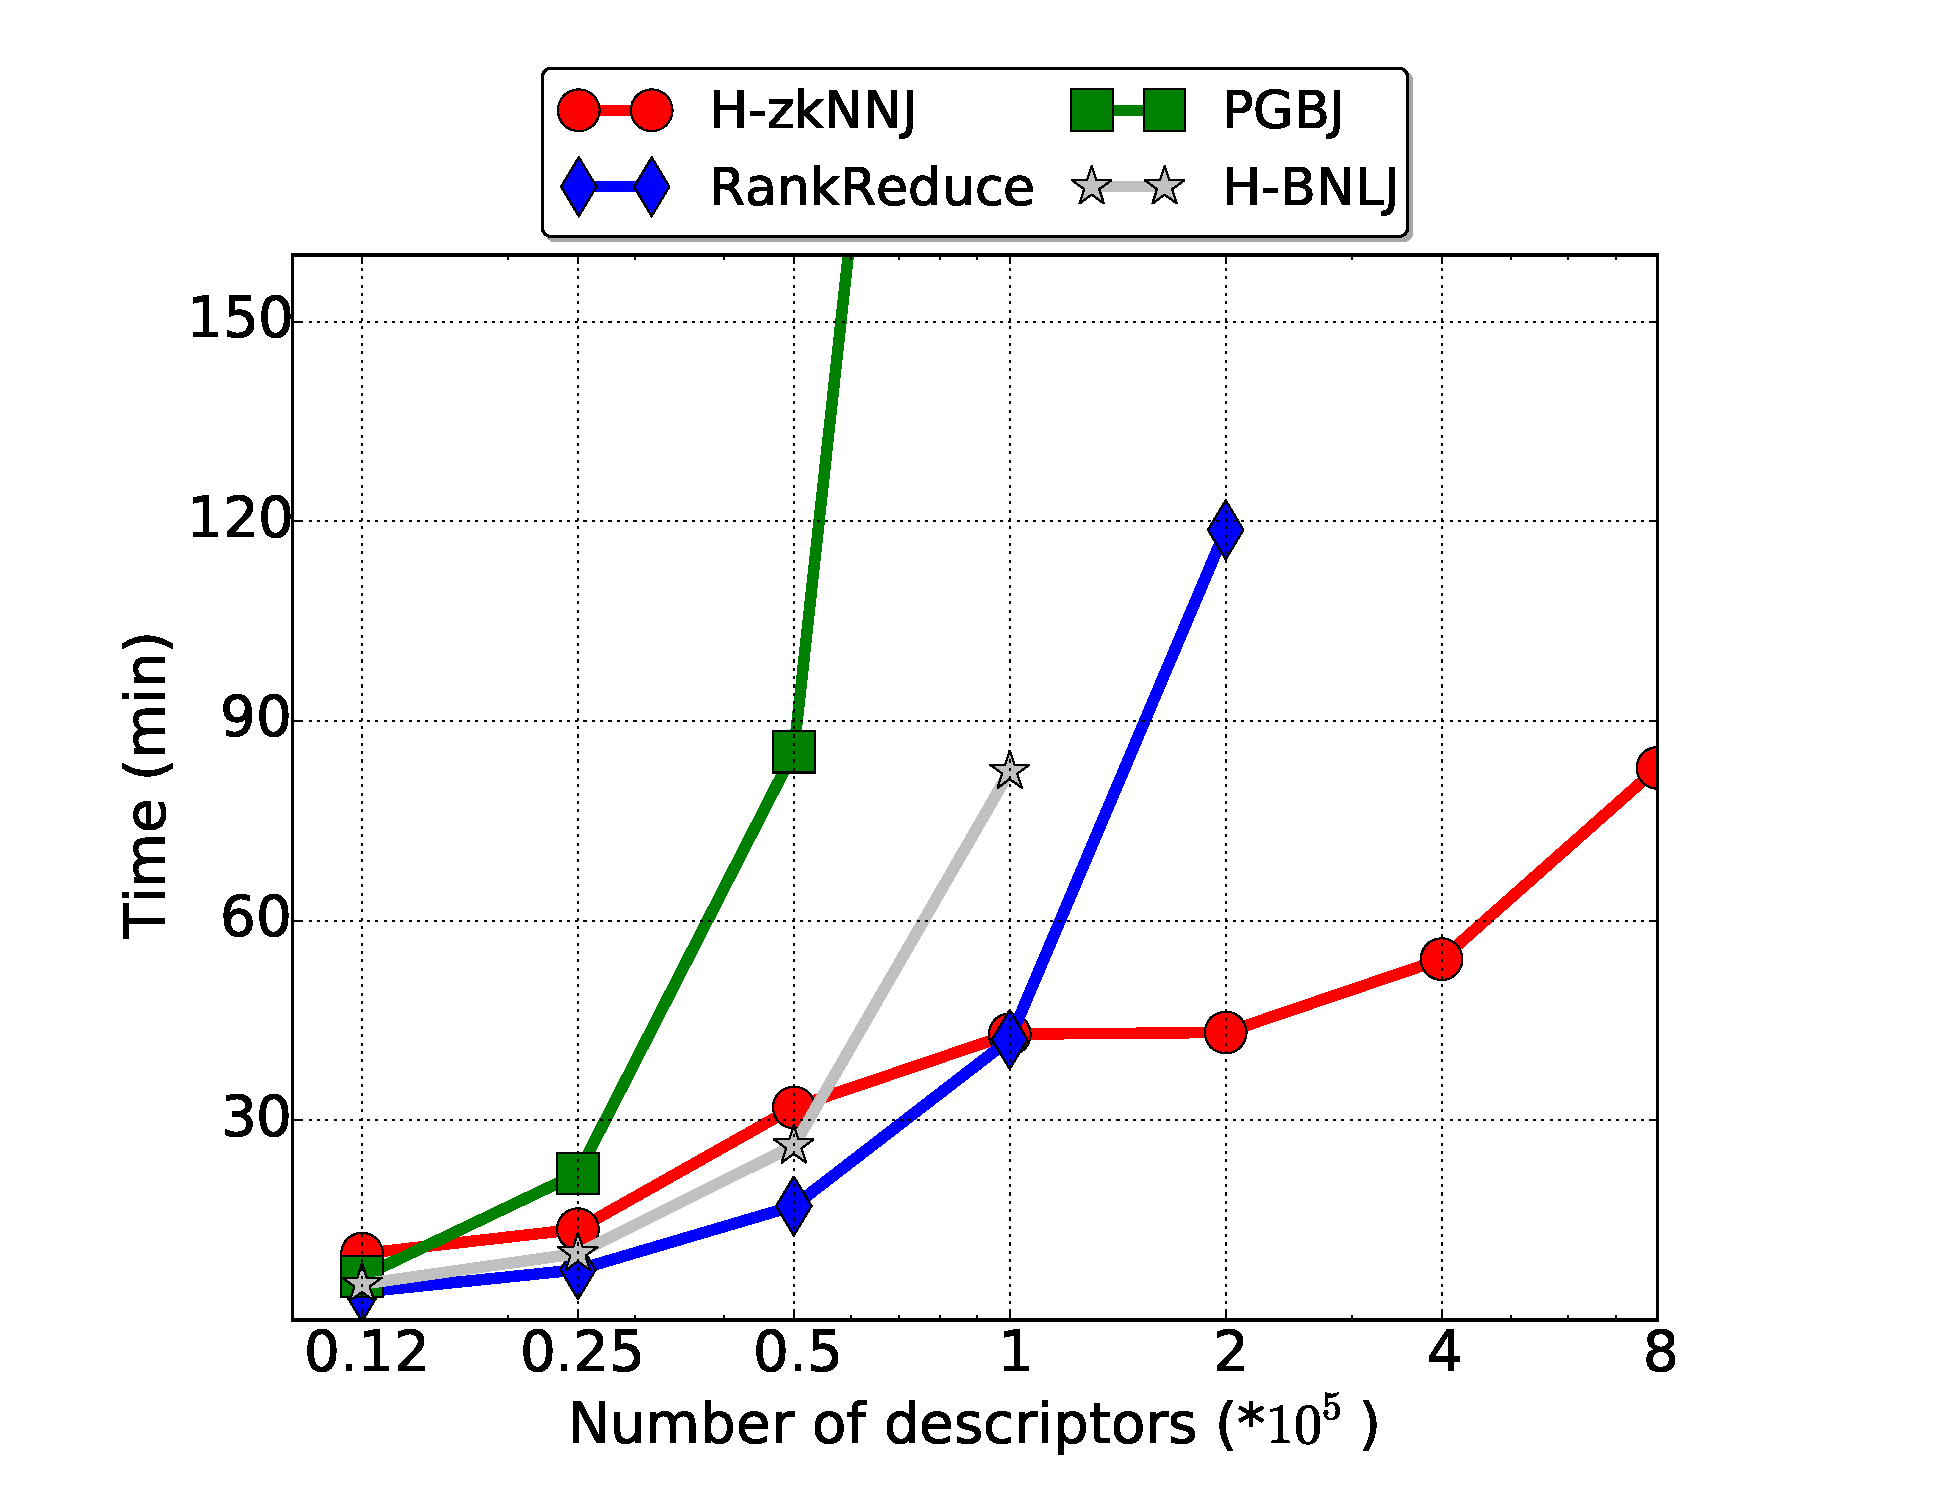
\includegraphics[width=\textwidth]{img-perf/surf/data/time.pdf}
		% }
		\caption{Time\label{fig:surf_data_time}}    
	\end{subfigure}%
	\begin{subfigure}[b]{0.35\textwidth}
		%\fbox{
		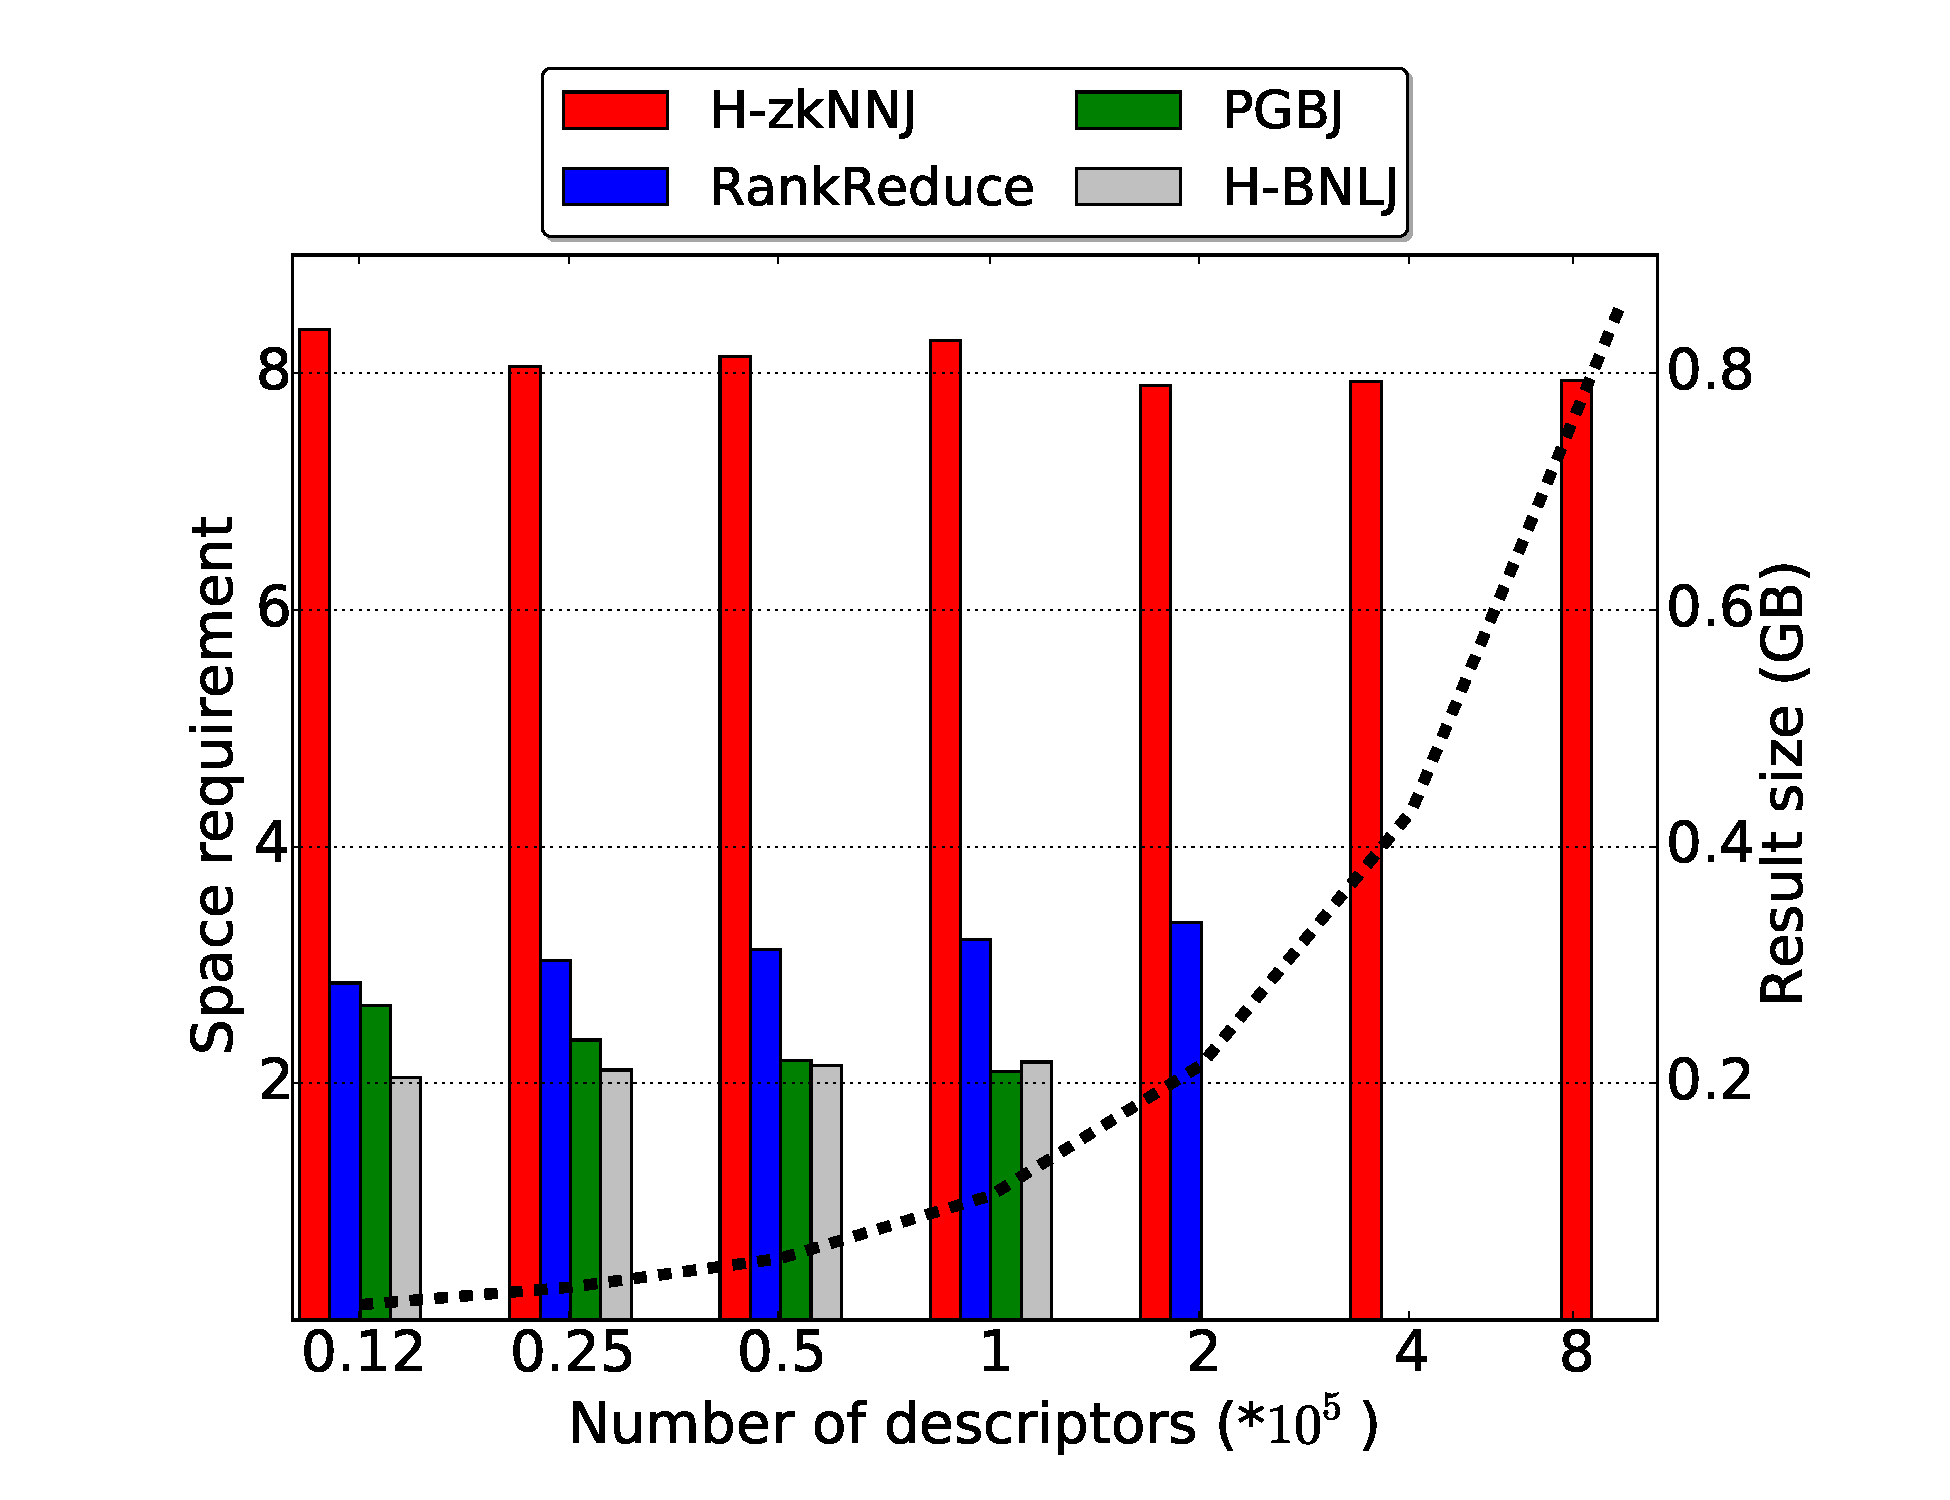
\includegraphics[width=\textwidth]{img-perf/surf/data/memory.pdf}
		%}
		\caption{Result size and Disk Usage\label{fig:surf_data_memory}}
	\end{subfigure}%       
	\begin{subfigure}[b]{0.35\textwidth}
		%\fbox{
		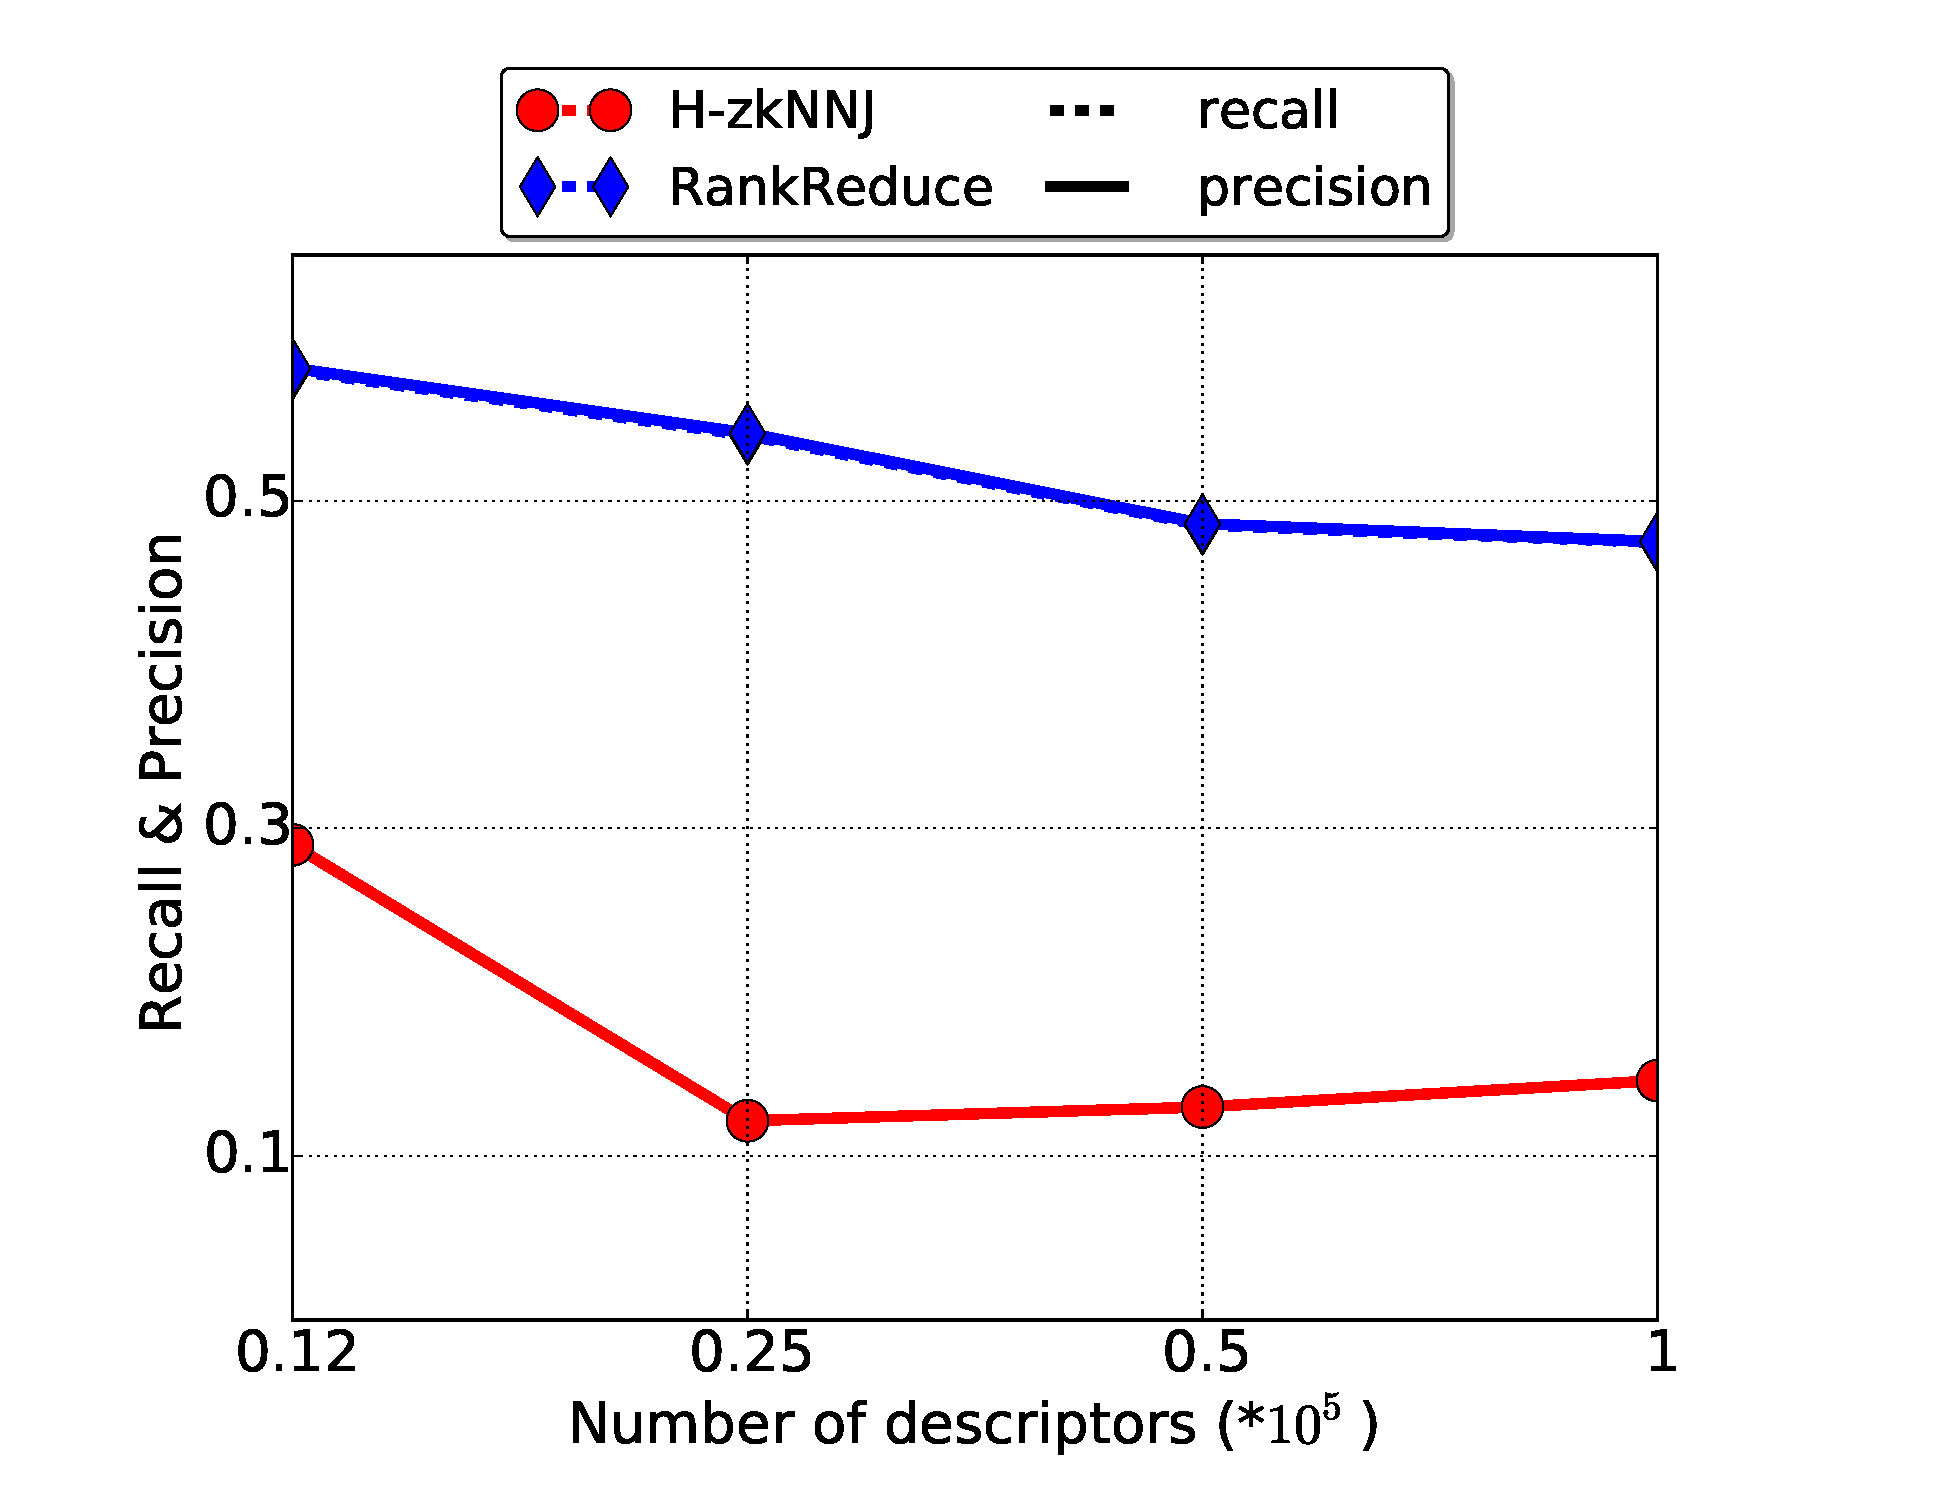
\includegraphics[width=\textwidth]{img-perf/surf/data/accuracy.pdf}
		%}
		\caption{Recall and Precision\label{fig:surf_data_acc}}        
	\end{subfigure}%  
	\caption{Surf, impact of the dataset size
		%\\ \small {Parameters : \textbf{HBNLJ} : 10partitions, \textbf{PGBJ}:$3*10^{3} pivots$, Geo grouping, kmeans 
		%sample, \textbf{RankReduce}: $L=5,M=7,W=10^{7}$ HZKNNJ : $3shift$} 
		\label{fig:surf_dataset} }
\end{figure*}

%%%% Generated by A4-ratioByK-SURF.py
\begin{figure*}[htp]
	\centering
	\begin{subfigure}[b]{0.35\textwidth}
		%\fbox{
		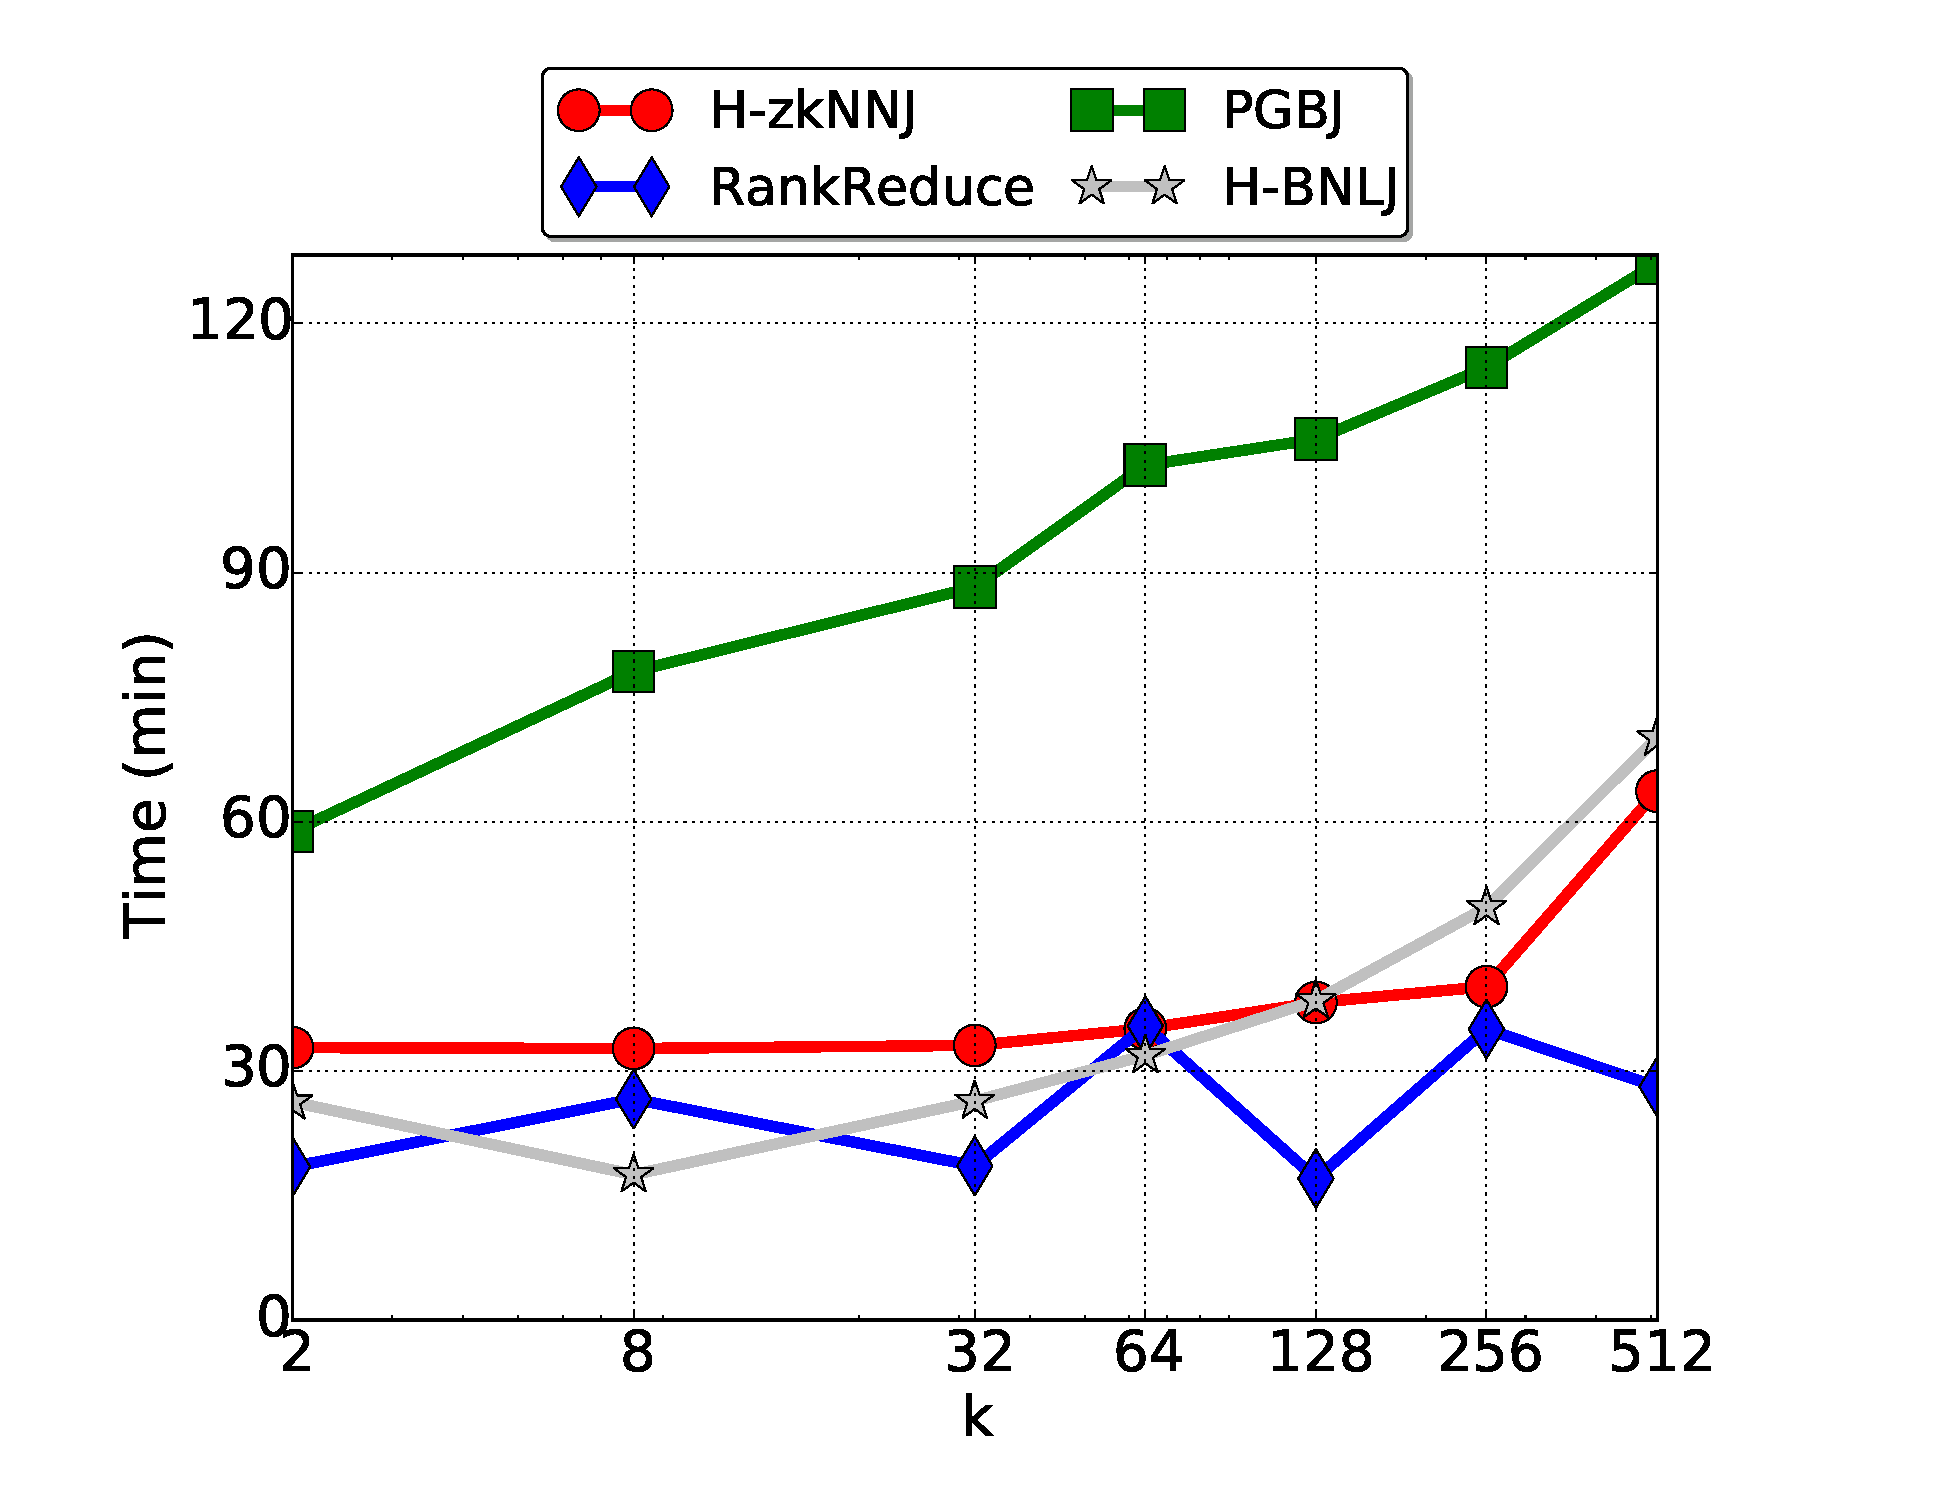
\includegraphics[width=\textwidth]{img-perf/surf/k/time.pdf} 
		%}
		\caption{Time\label{fig:surf_k_time} }
		
	\end{subfigure}%
	\begin{subfigure}[b]{0.35\textwidth}
		% \fbox{
		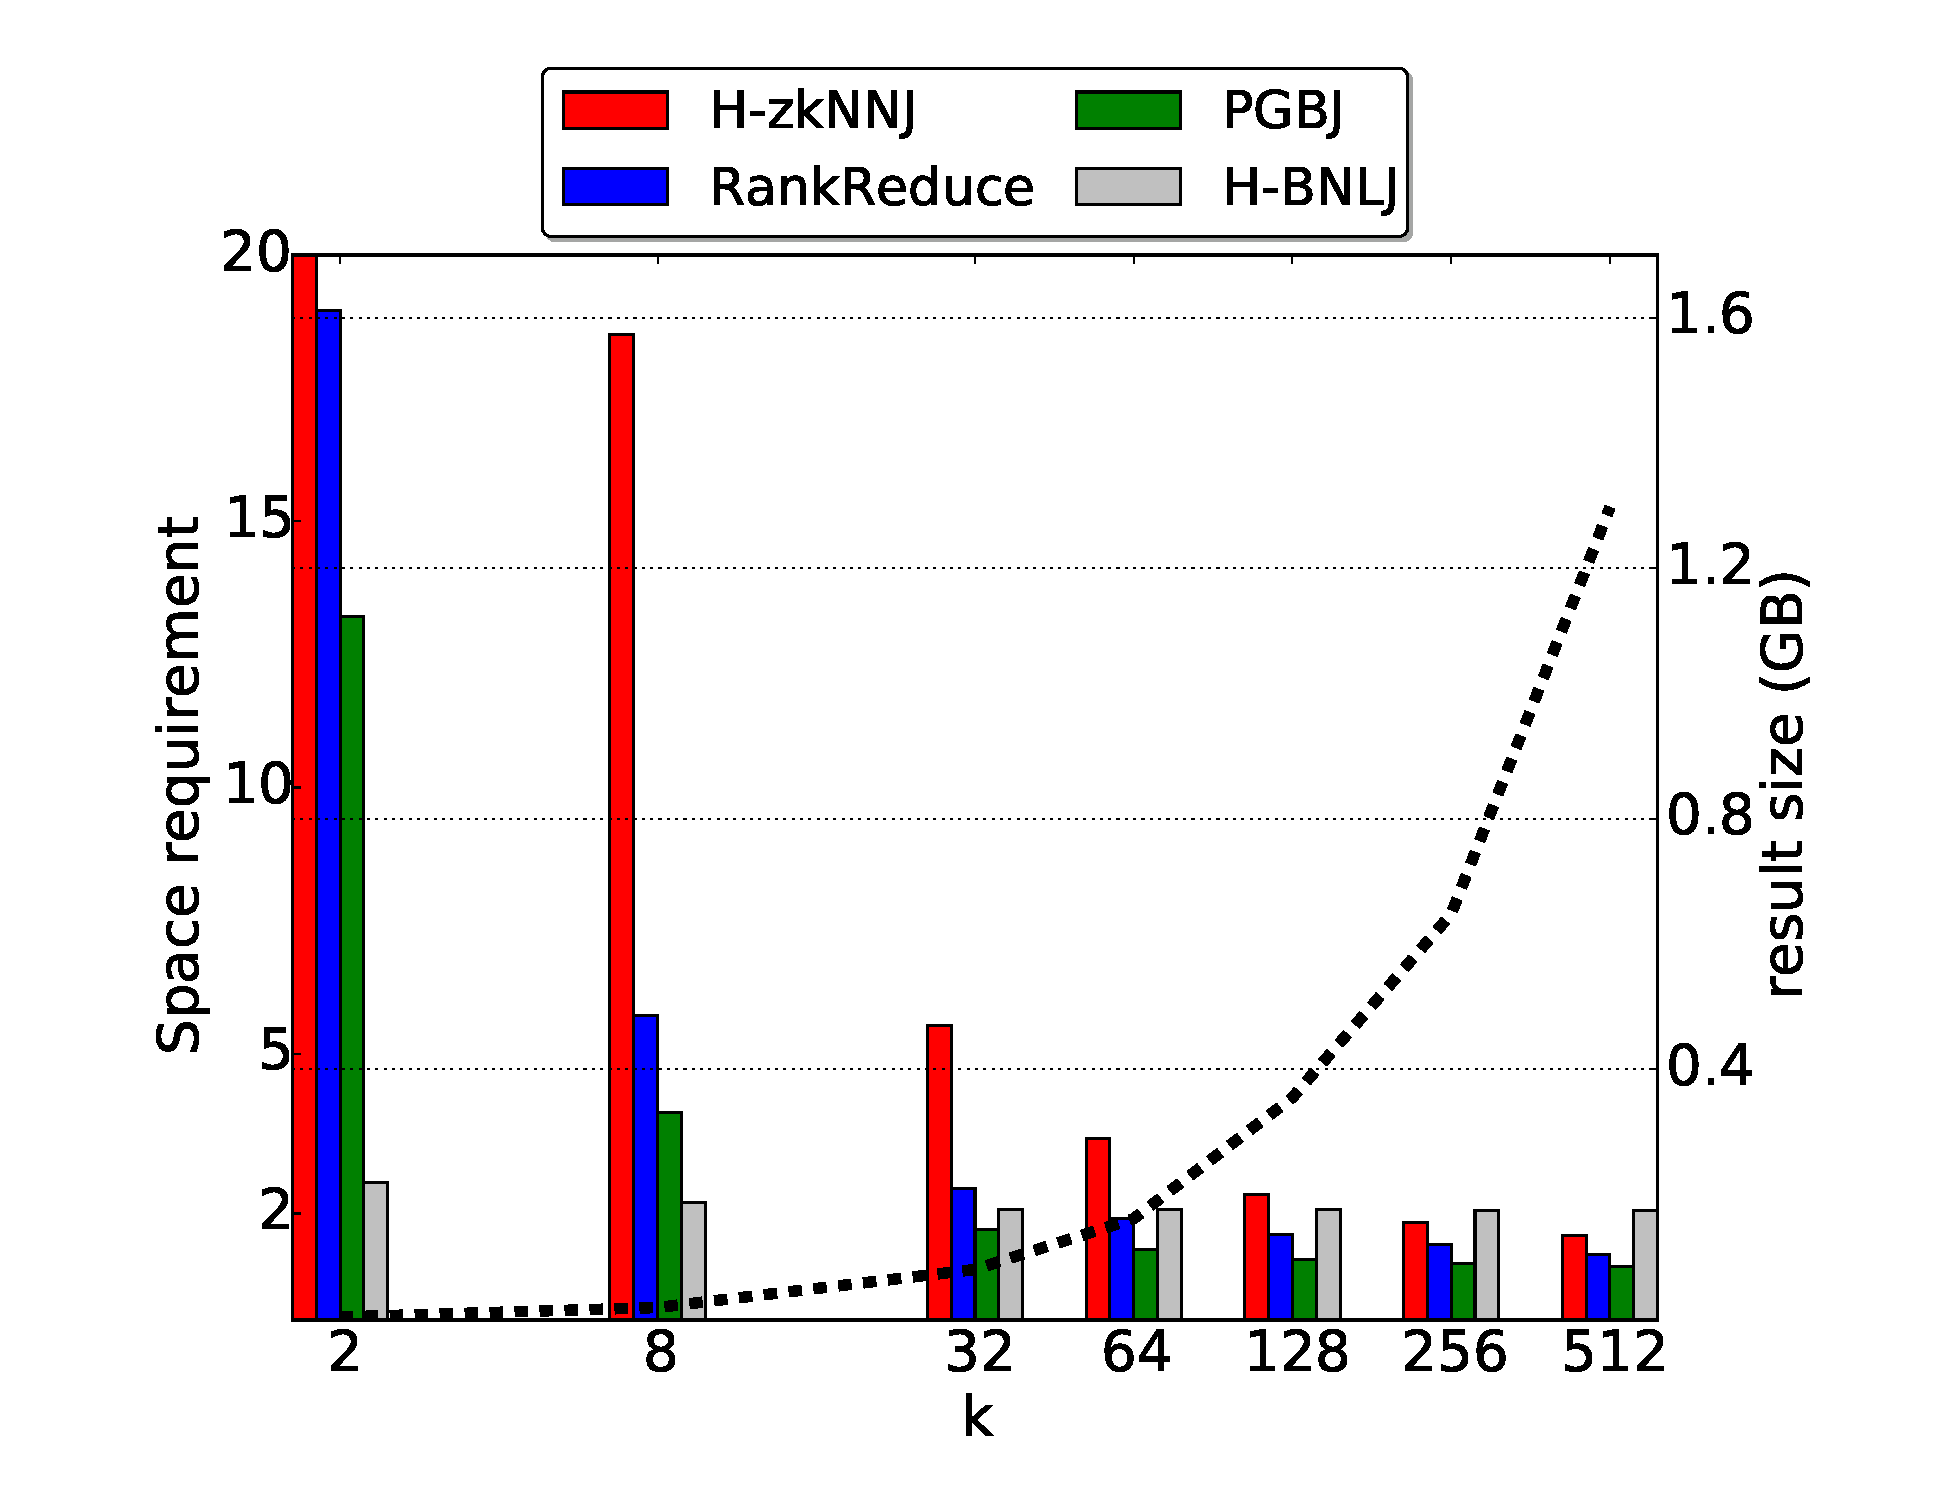
\includegraphics[width=\textwidth]{img-perf/surf/k/memory.pdf} 
		%}
		\caption{Result size and Disk Usage\label{fig:surf_k_memory}}
	\end{subfigure}%
	\begin{subfigure}[b]{0.35\textwidth}
		%\fbox{
		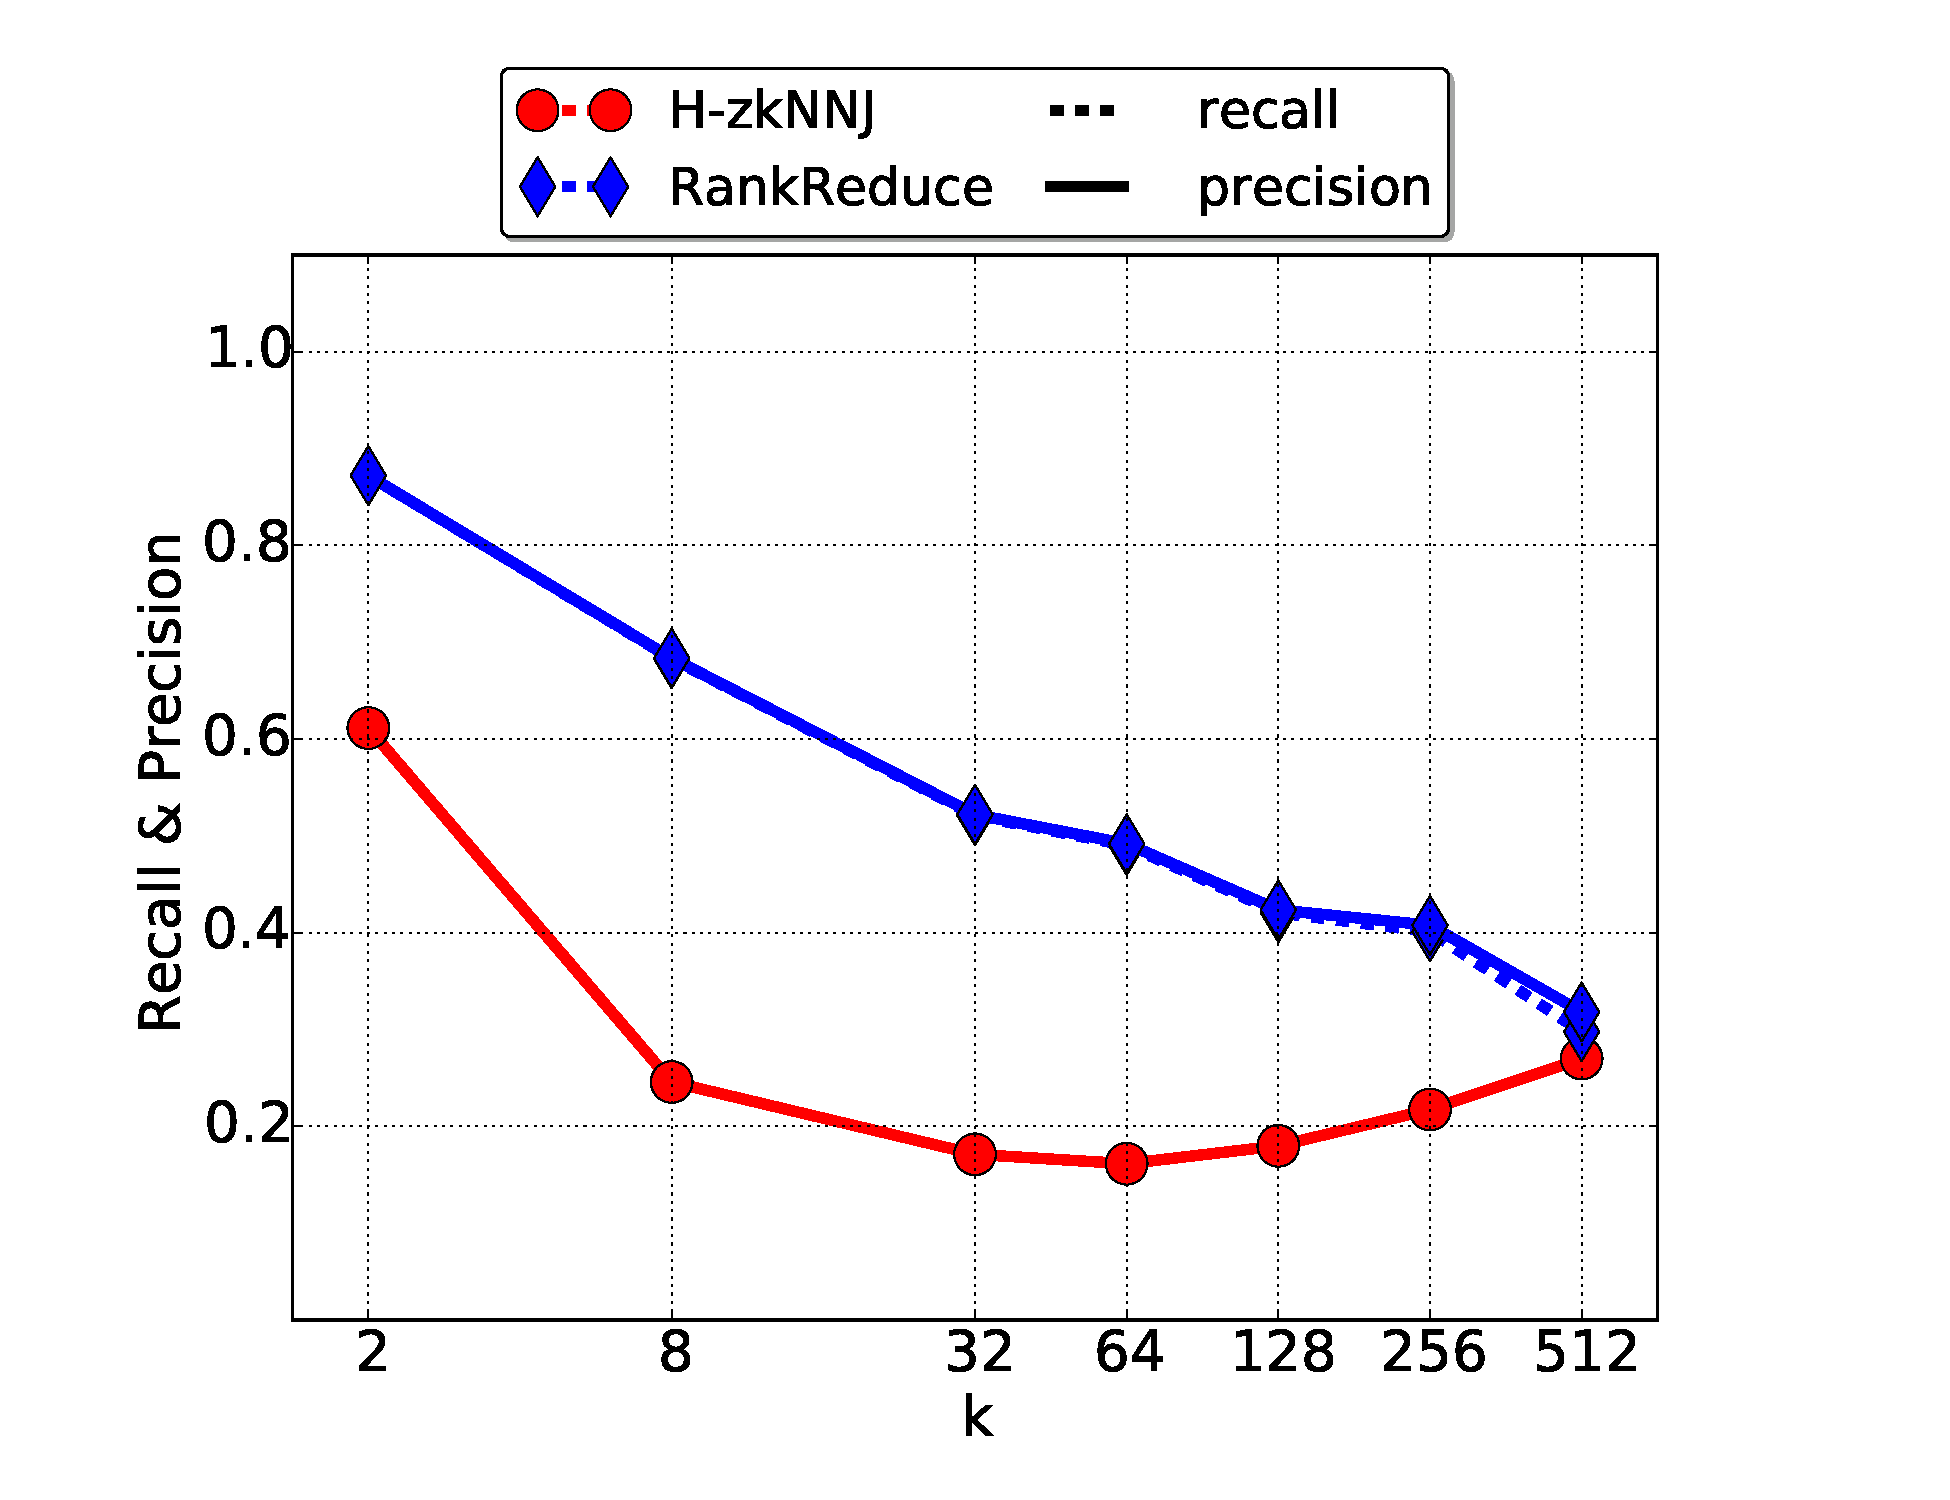
\includegraphics[width=\textwidth]{img-perf/surf/k/accuracy.pdf}
		%}
		\caption{Recall and Precision\label{fig:surf_k_acc}}
		
	\end{subfigure}%
	\caption{Surf dataset with 50k records, impact of $K$,
		%\\ \small{Parameters : \textbf{HBNLJ} : 10partition, \textbf{PGBJ}:$3*10^3 pivots$, Geo grouping, kmeans 
		%sample,\textbf{RankReduce}: $L=5,M=7,W=10^7$ HZKNNJ : $3shift$}  
		\label{fig:surf_impact_k}}
\end{figure*}


\subsubsection{Impact of input data size}

Results of experiments when varying the number of descriptors are shown in Figure~\ref{fig:surf_dataset} using a log 
scale on the x-axis. We omitted \HBK~as it could not process the data in reasonable time.
In Figure~\ref{fig:surf_data_time}, we can see that the execution time of the algorithms follows globally 
the same trend as 
with the Geo dataset, except for \VO. It is a computational intensive algorithm because the replication process implies 
calculating a lot of Euclidian distances. When in dimension 128, this part tends to dominate the overall computation 
time. Regarding disk usage (Figure~\ref{fig:surf_data_memory}), \Z~is very high because  we had to increase the number 
of shifted copies from $3$ to $5$ to 
improve the recall. Indeed, compared to the Geo dataset, it is very low (Figure~\ref{fig:surf_data_acc}). Moreover, as 
the number of descriptors 
increases, \Z~goes from 30\% to 15\% recall. As explained before, the precision was found to be equal to the recall, which means the 
algorithm always returned $k$ results. This, together with the improvement using more shifts, proves that the 
space filling curves using in \Z~are less efficient with high dimension data. 
%A solution is to 
%increase the number of shifted copies from $3$ to $5$. But the impact of time is double and no very efficient, it 
%increases just to $0.05$ the recall . \TODO{I'm confused, was the shift increased or not?}

\subsubsection{Impact of $k$}

Figure \ref{fig:surf_impact_k} shows the impact of different values of $k$ on the algorithms using a logarithmic scale 
on the x-axis.
Again, since for \HBNLJ~and \Z, the complexity of the sorting phase is dependent on $k$, we can observe a 
corresponding increase of the execution time (Figure~\ref{fig:surf_k_time}). For 
\LSH, the time varies a lot depending on $k$. This is because of the stochastic nature of the projection used in 
LSH. It can lead to buckets containing different number of elements, creating a load imbalance and some values
of $k$ naturally lead to a better load balancing. \VO~is very dependent on the value of $k$ because of the grouping 
phase. Neighboring cells are added until there are enough elements to eventually identify the $k$ nearest neighbors. 
As a consequence, a large $k$ will lead to larger group of cells and increase the computing time. 

Figure~\ref{fig:surf_k_memory} shows the effect of $k$ on disk usage. \Z~starts with a very high ratio of 74 
(not showed on the Figure) and 
quickly reduces to more acceptable values. 
 \LSH~also experiences a similar pattern to a lesser extend. As opposed to the Geo dataset, SURF 
descriptors cannot be efficiently compressed, leading to large intermediate files.

Finally, Figure~\ref{fig:surf_k_acc} shows the effect of $k$ on the recall. As $k$ increases, the recall and precision 
of \LSH~ decreases for the same reason as with the Geo dataset. Also, for large $k$, the recall becomes lower
than the precision because we get less than $k$ results. The precision of \Z~decreases but eventually shows an upward 
trend. The increased number of requested neighbors increases the number of preceding and
succeeding points copied, slightly improving the recall.
%  the number of searched $k$ reduce the probability to make 
%mistake and, 
%contrarily to \LSH, no $k$ is missing in the result (recall = precision) \TODO{Rewrite}

\subsubsection{Communication Overhead}
With the SURF dataset, we get a very different behavior than with the Geo dataset. The shuffle phase of \VO~is very 
costly (Figure~\ref{fig:surf_data_shuffle}). This is an indication of large replications incurred by the large 
dimension of the data and a poor choice of pivots. When they are too close to each other, entire cells have to be 
replicated during the grouping phase.

%%%% Generated by B00-surf.py and A4-ratioByK-SURF.py
\begin{figure*}[htp]
	\centering
	\begin{subfigure}[b]{0.48\textwidth}
		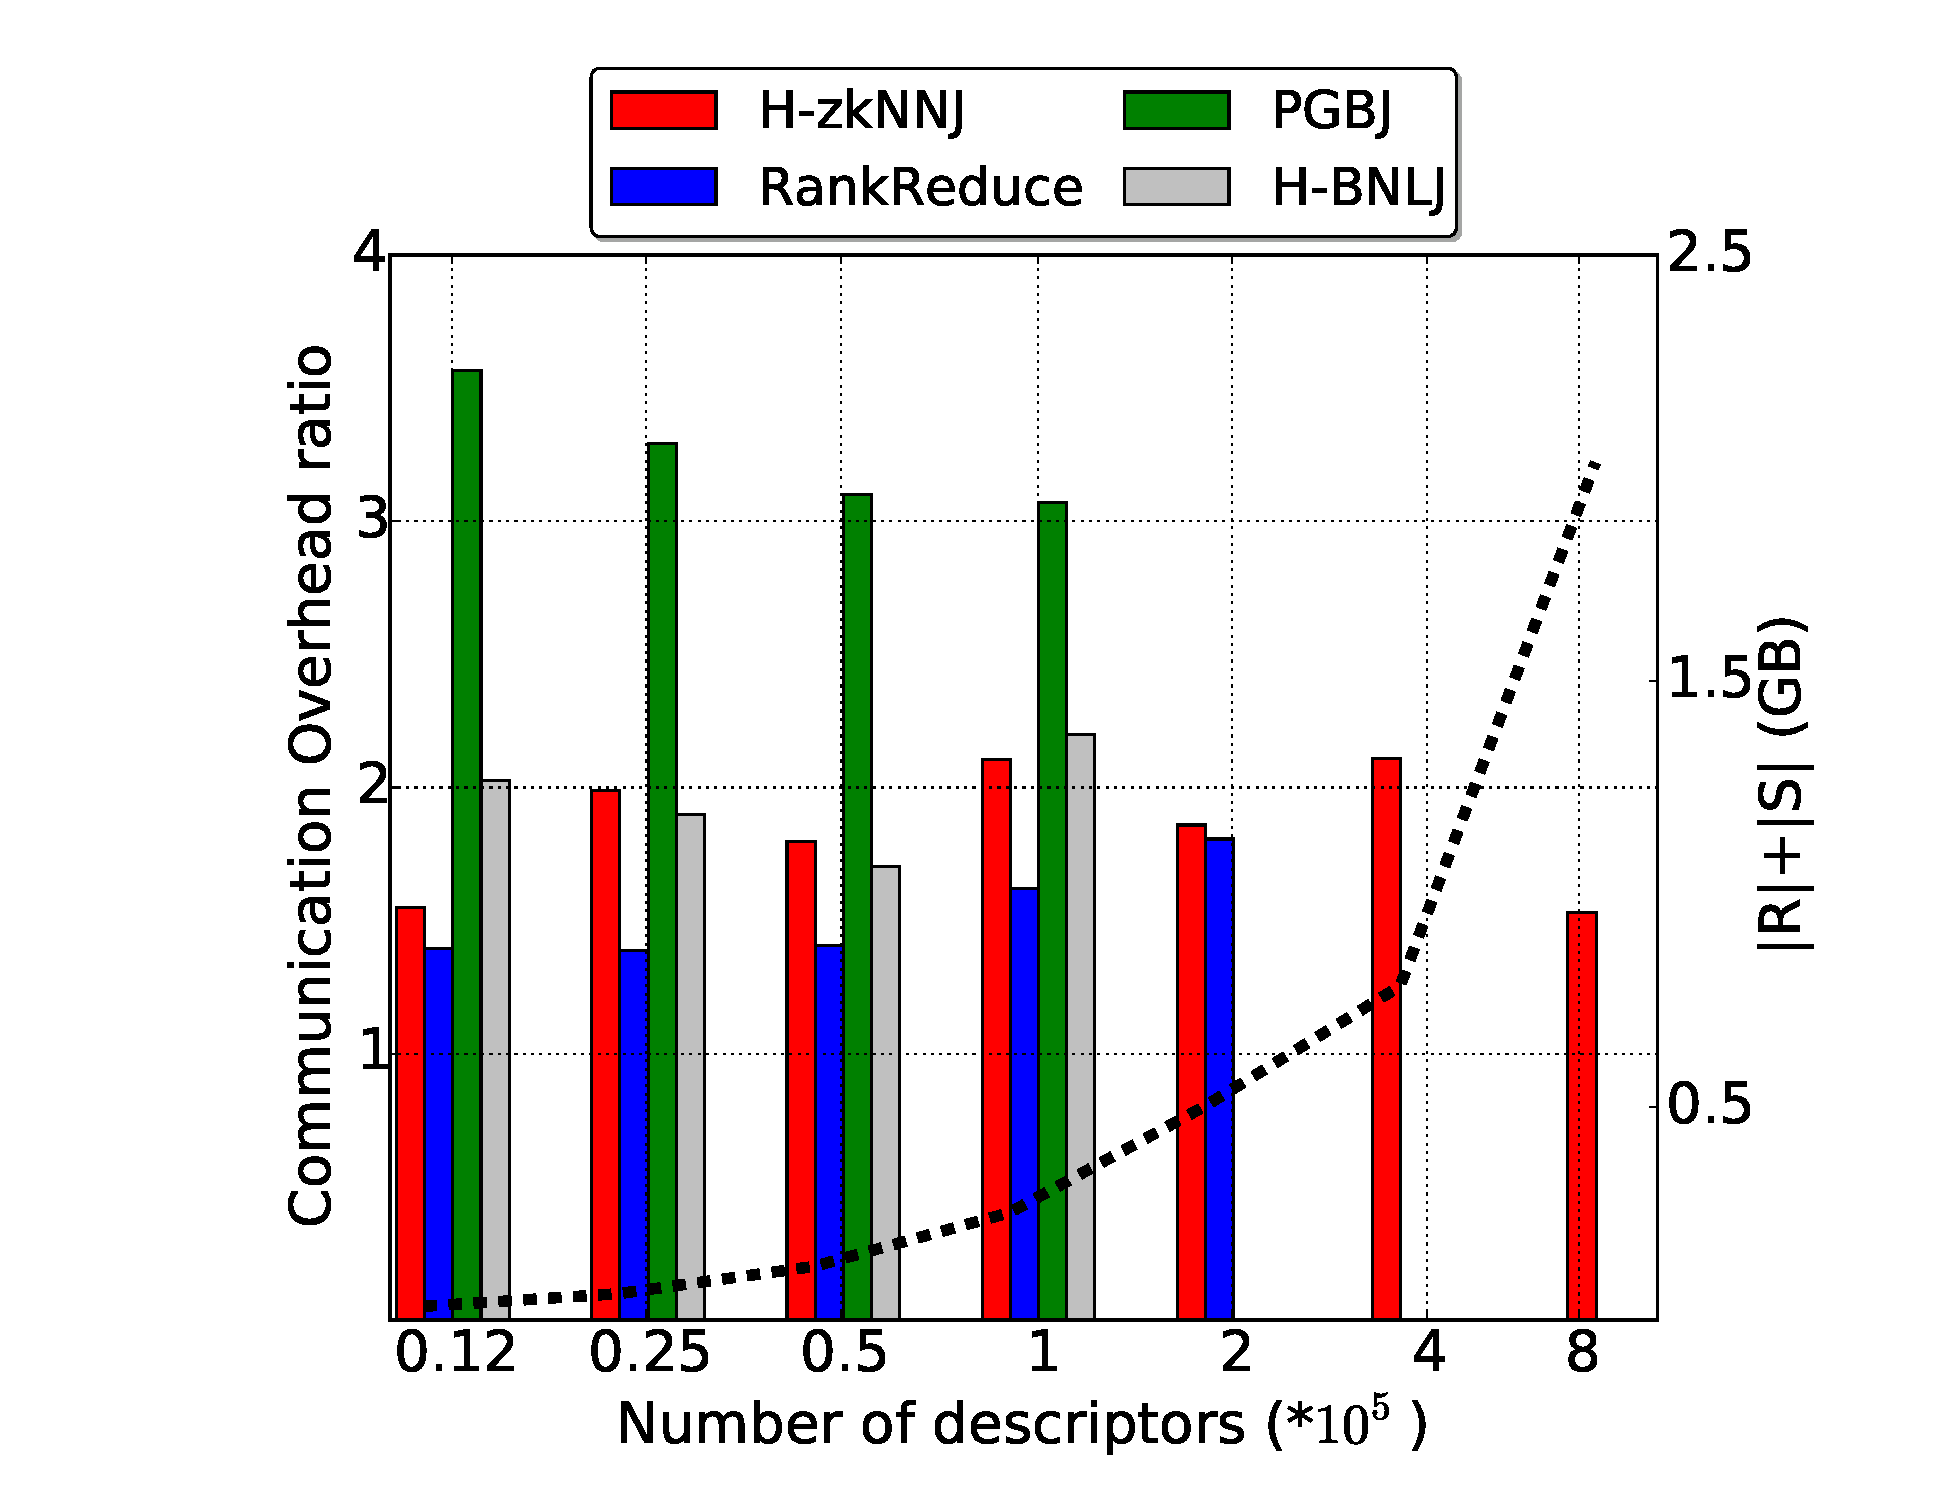
\includegraphics[width=\textwidth]{img-perf/surf/data/shuffle.pdf}
		\caption{Surf, impact of the dataset size\label{fig:surf_data_shuffle}}        
	\end{subfigure}% 
	\begin{subfigure}[b]{0.48\textwidth}
		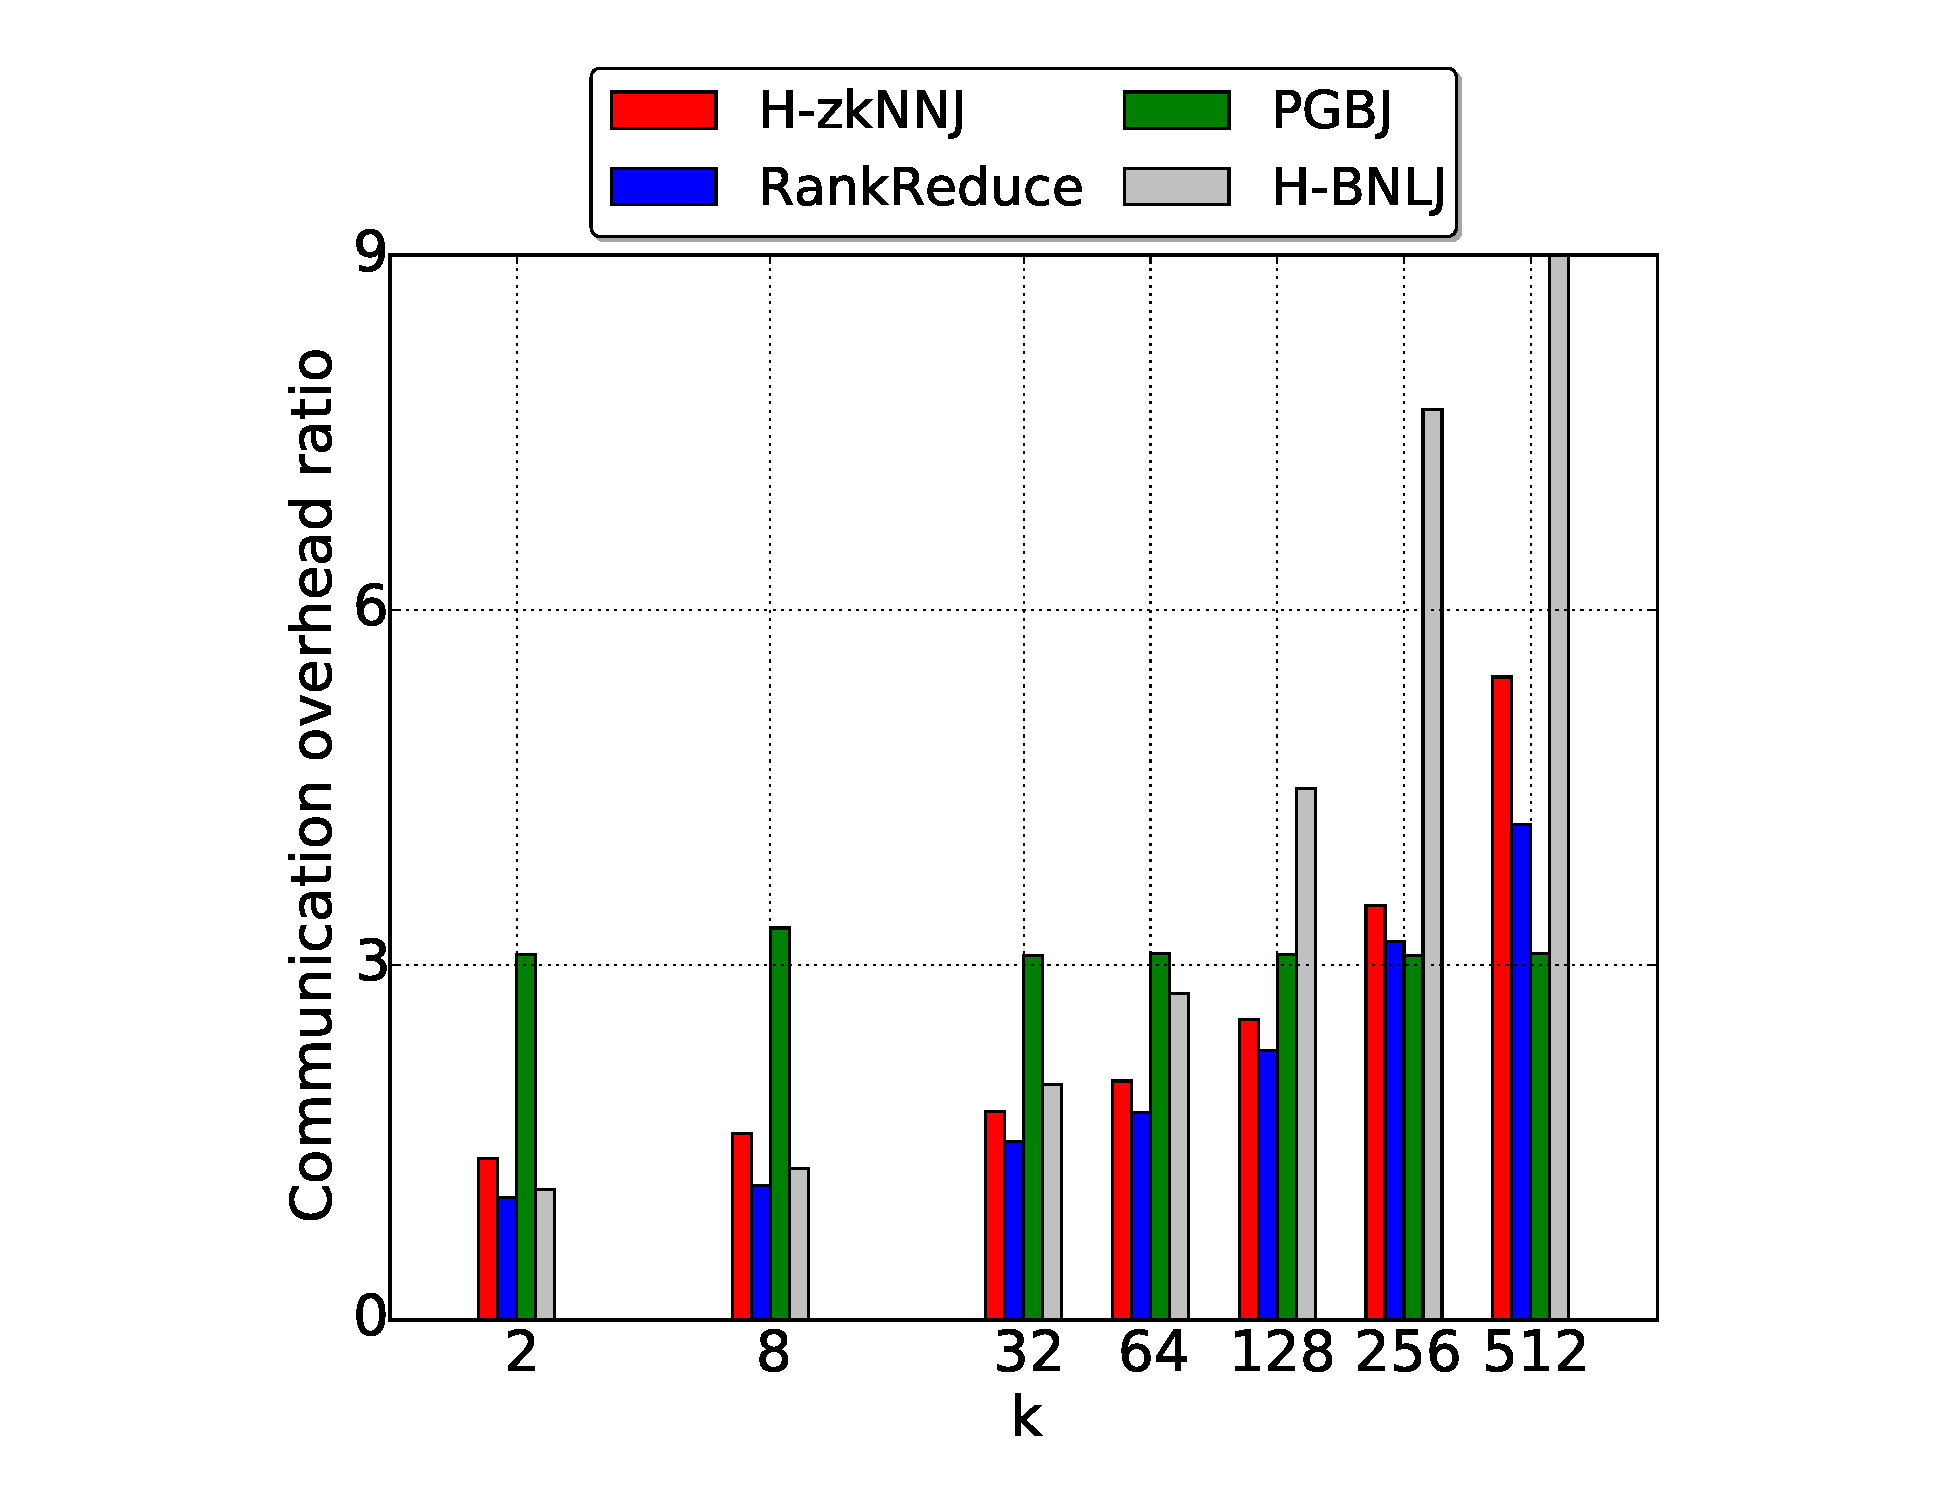
\includegraphics[width=\textwidth]{img-perf/surf/k/shuffle.pdf} 
		\caption{Surf dataset with 50k records, impact of $K$,\label{fig:surf_k_shuffle}}
	\end{subfigure}%
	\caption{Communication overhead for the Surf dataset}      
\end{figure*}


For \LSH~the shuffle is decreased but stay important, essentially because of the replication factor of $5$. Finally,
the shifts of original data in \Z~lead to a large communication overhead. 


Considering now $k$, we have the same behavior we observed with the Geo dataset. The only difference is \VO~which now exhibits a
large communication overhead (Figure~\ref{fig:surf_k_shuffle}). This is again because of the choice of pivots and 
the grouping of the cells. However, this overhead remains constant, irrespective of $k$. 

\subsection{Impact of Dimension and Dataset}
We now analyze the behavior of these algorithms according to the dimension of  data. Since 
some algorithms are dataset dependent (i.e the spatial distribution of data has an impact on 
the outcome), we need to separate data distribution from the dimension. Hence, we use two
different kinds of datasets for these experiments. First, we use real world data of various 
dimensions\footnote{archive.ics.uci.edu/ml/datasets.html}. Second, we have built specific datasets by generating 
uniformly distributed data to limit the impact of clustering. All the experiments were performed using 
$0.5*10^5$ records and $k=20$. 
 
%
% \begin{table}[h]
% 	\begin{center}
% 		\begin{tabular}{|c|c|c|}
% 			\hline 
%% 			& \multicolumn{2}{|c|}{Size} \\
%% 			\cline{2-3}
% 			Dimension & Real & Synthetic \\
% 			\hline
% 			2 & 7.1MB & 846KB \\
% 			9 & 3.5MB & 2.8MB \\
% 			28 & 35MB & 8MB  \\
% 			77& 23MB & 21MB \\
% 			128 & 63MB & 36MB  \\
% 			281 & 60MB & 78MB\\
% 			386 & 73MB & 107MB  \\
% 			\hline
% 		\end{tabular}
%% 		\caption{Size of $0.5*10^{5}$ records for $R$ and $S$ in dimension experiments\label{table:datasetup_dim}
% 			\TODO{Do we keep it?}}
% 	\end{center}
% \end{table}
 



%%%% Generated by 3-dim.py
\begin{figure*}[ht]
	\centering
	\begin{subfigure}[b]{0.5\textwidth}
		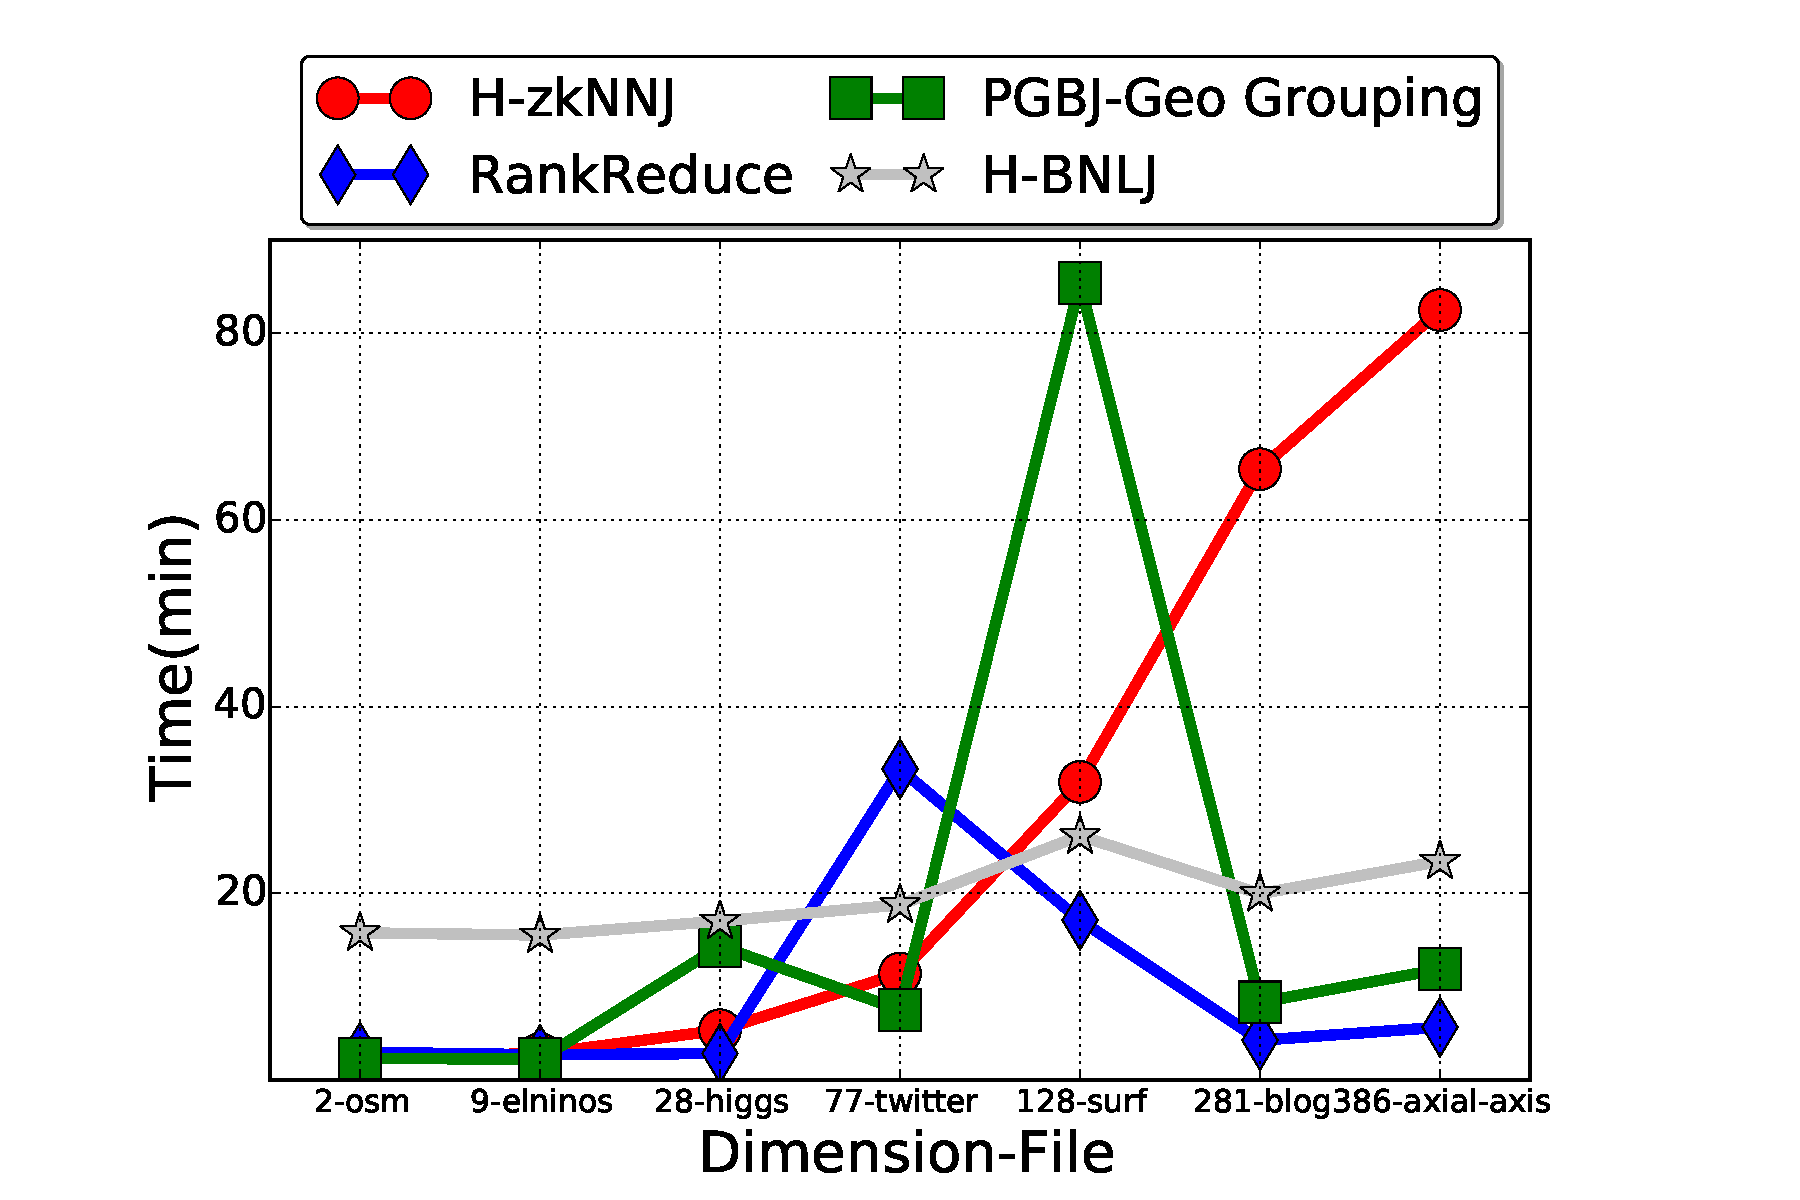
\includegraphics[width=1\textwidth]{img-perf/dim/datasettime.pdf} 
		\caption{Execution time% for real datasets of various dimensions%
		}
		\label{fig:dim_time}
	\end{subfigure}\begin{subfigure}[b]{0.5\textwidth}
	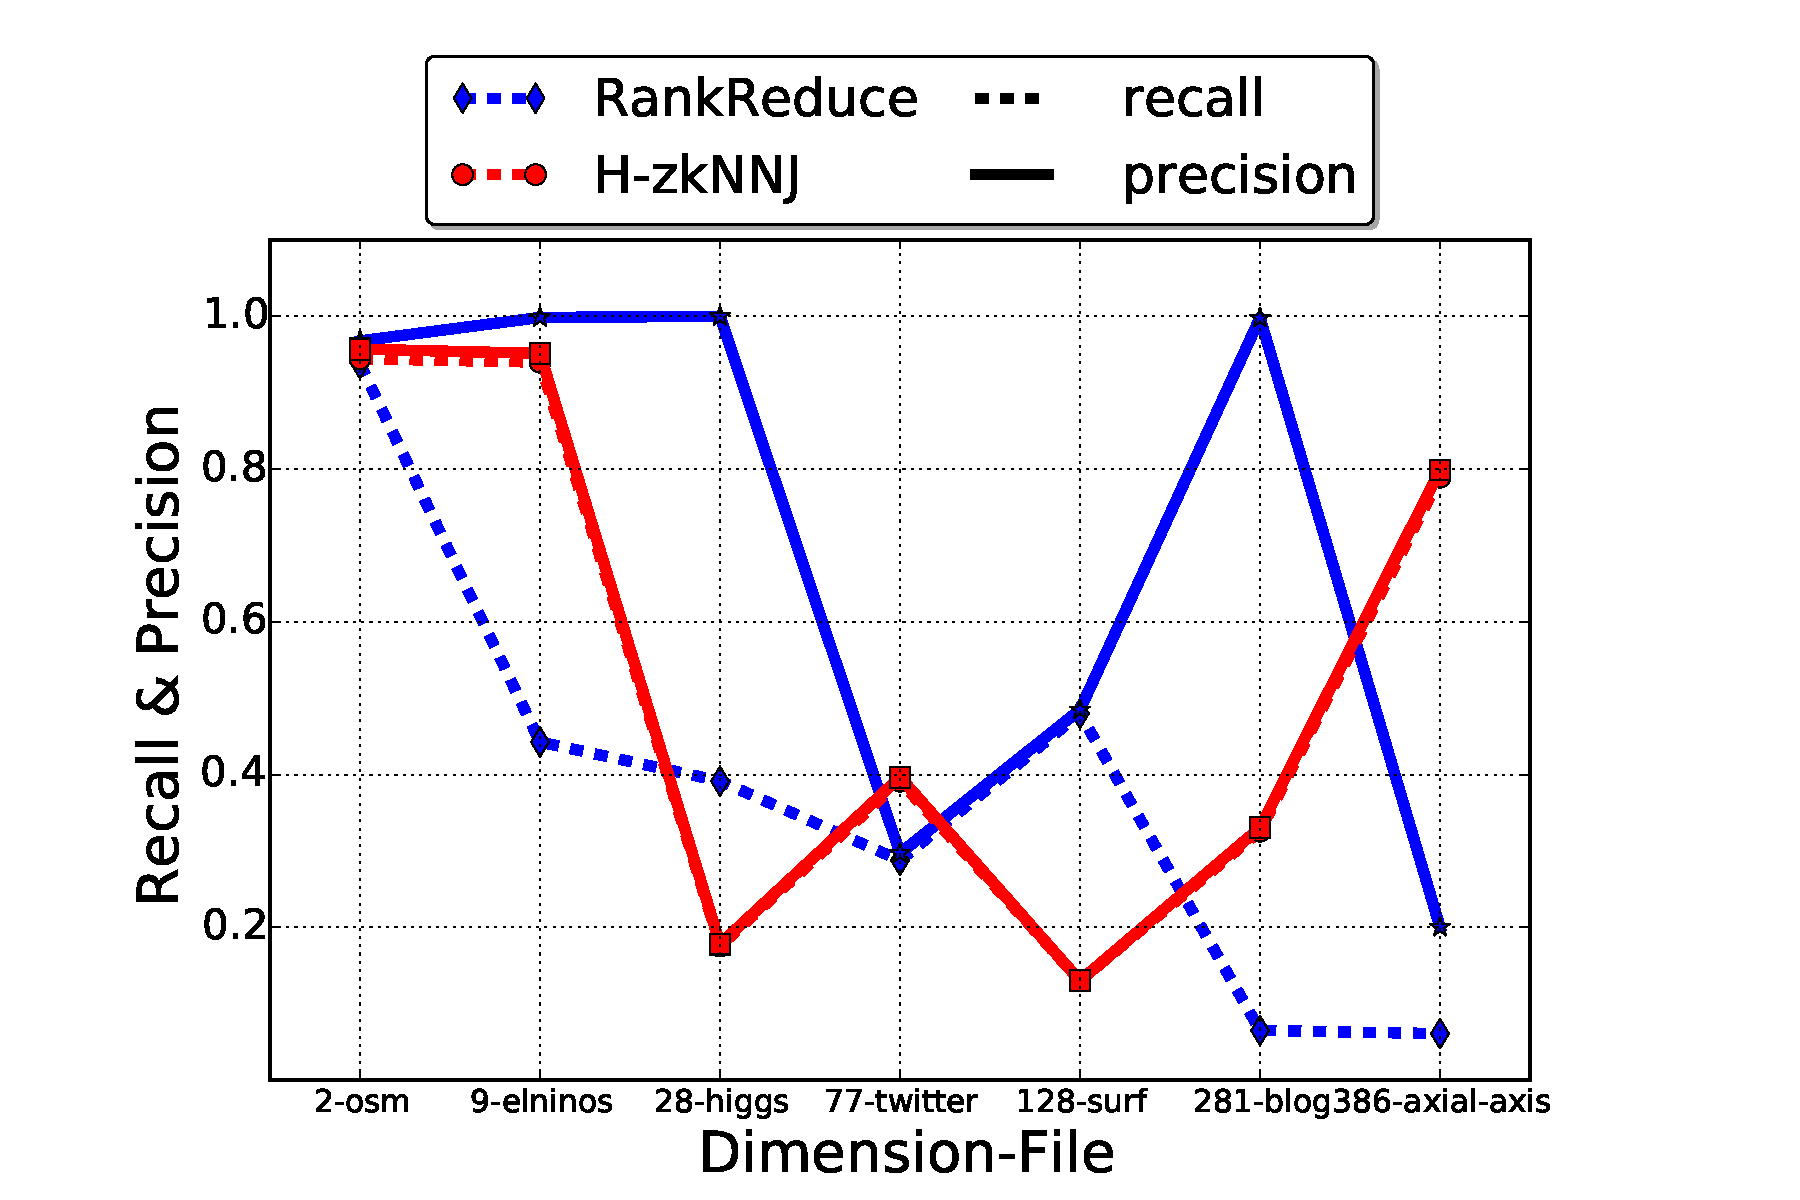
\includegraphics[width=1\textwidth]{img-perf/dim/datasetacc.pdf} 
	\caption{Recall and Precision %for real datasets of various dimensions%
	}
	\label{fig:dim_acc}
\end{subfigure}%
\caption{Real datasets of various dimensions}
\label{fig:dim_real}
\end{figure*} 

\begin{figure*}[ht]
	\centering
	\begin{subfigure}[b]{0.5\textwidth}
		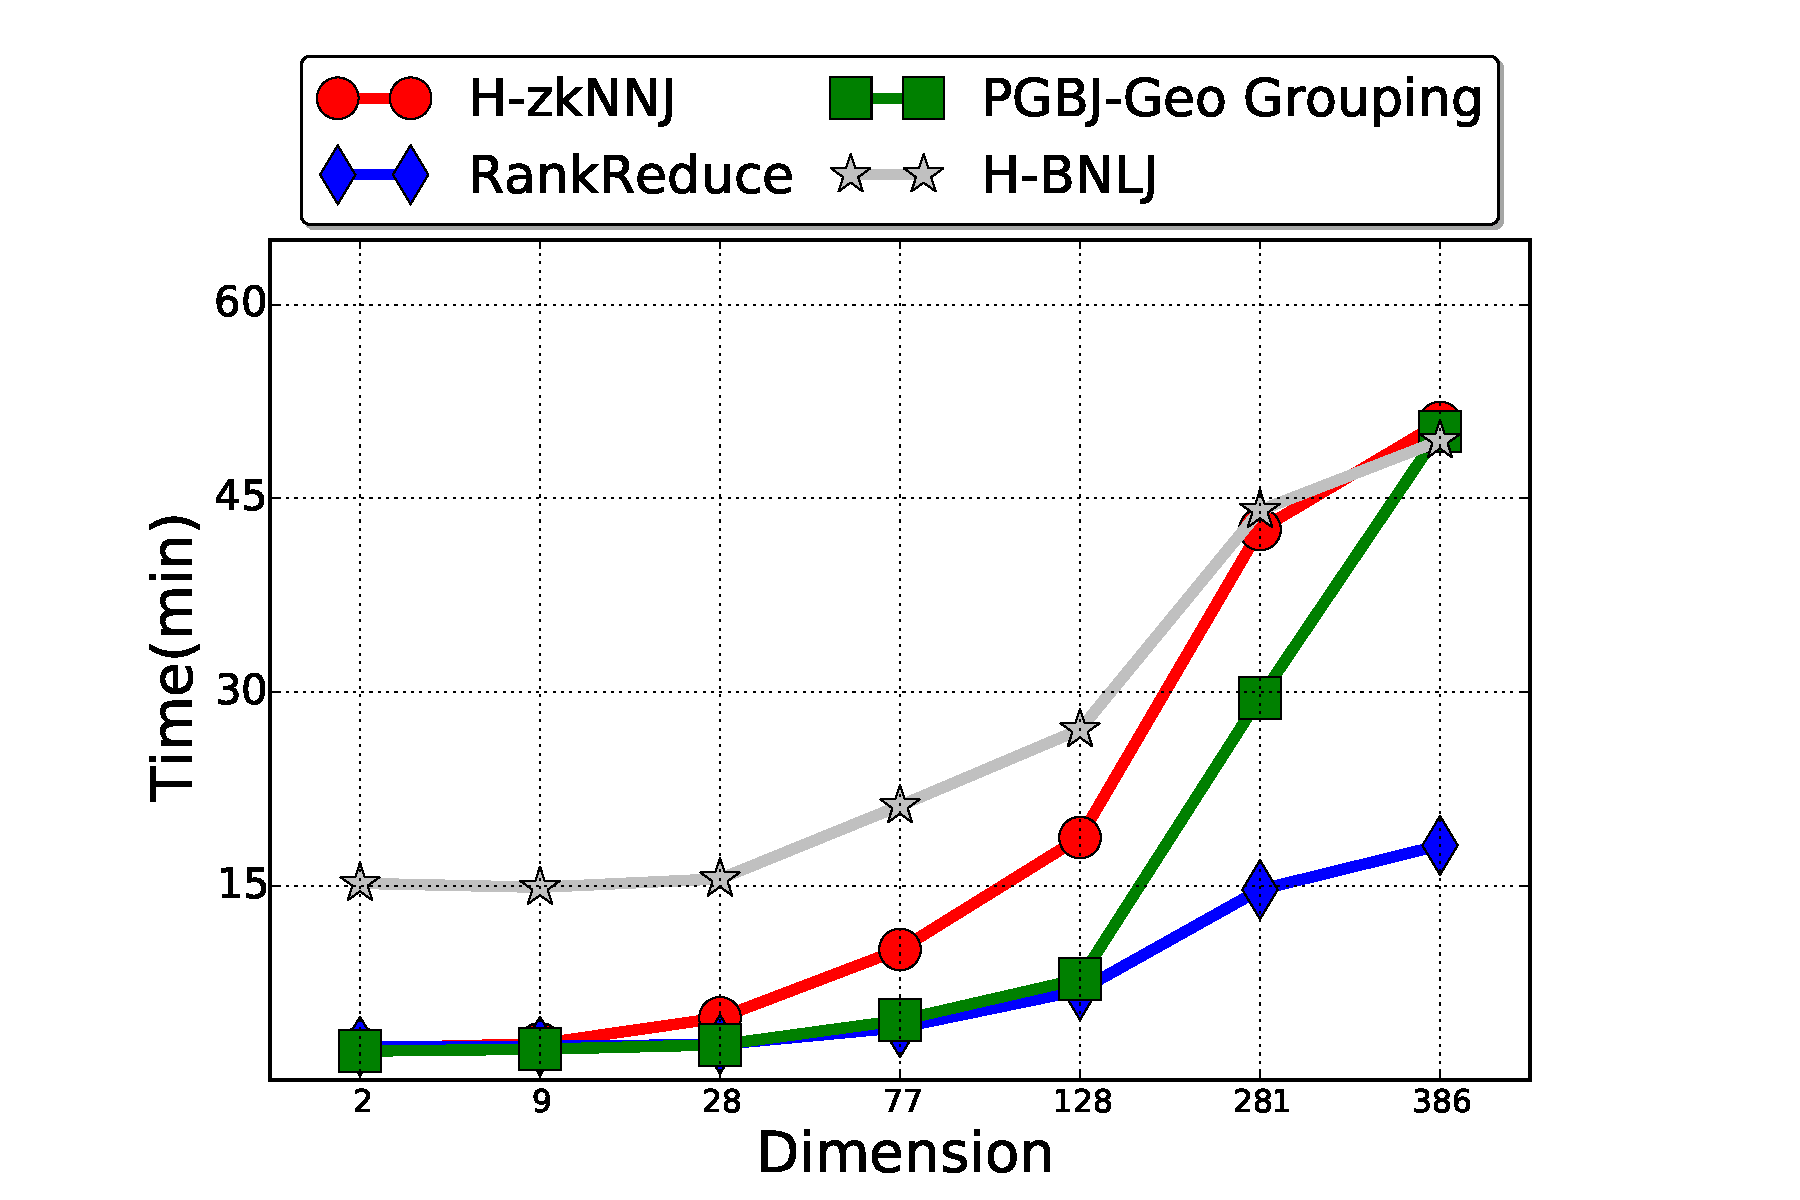
\includegraphics[width=1\textwidth]{img-perf/dim/randtime.pdf} 
		\caption{Execution time% for real datasets of various dimensions%
		}
		\label{fig:rand_time}
	\end{subfigure}\begin{subfigure}[b]{0.5\textwidth}
	
	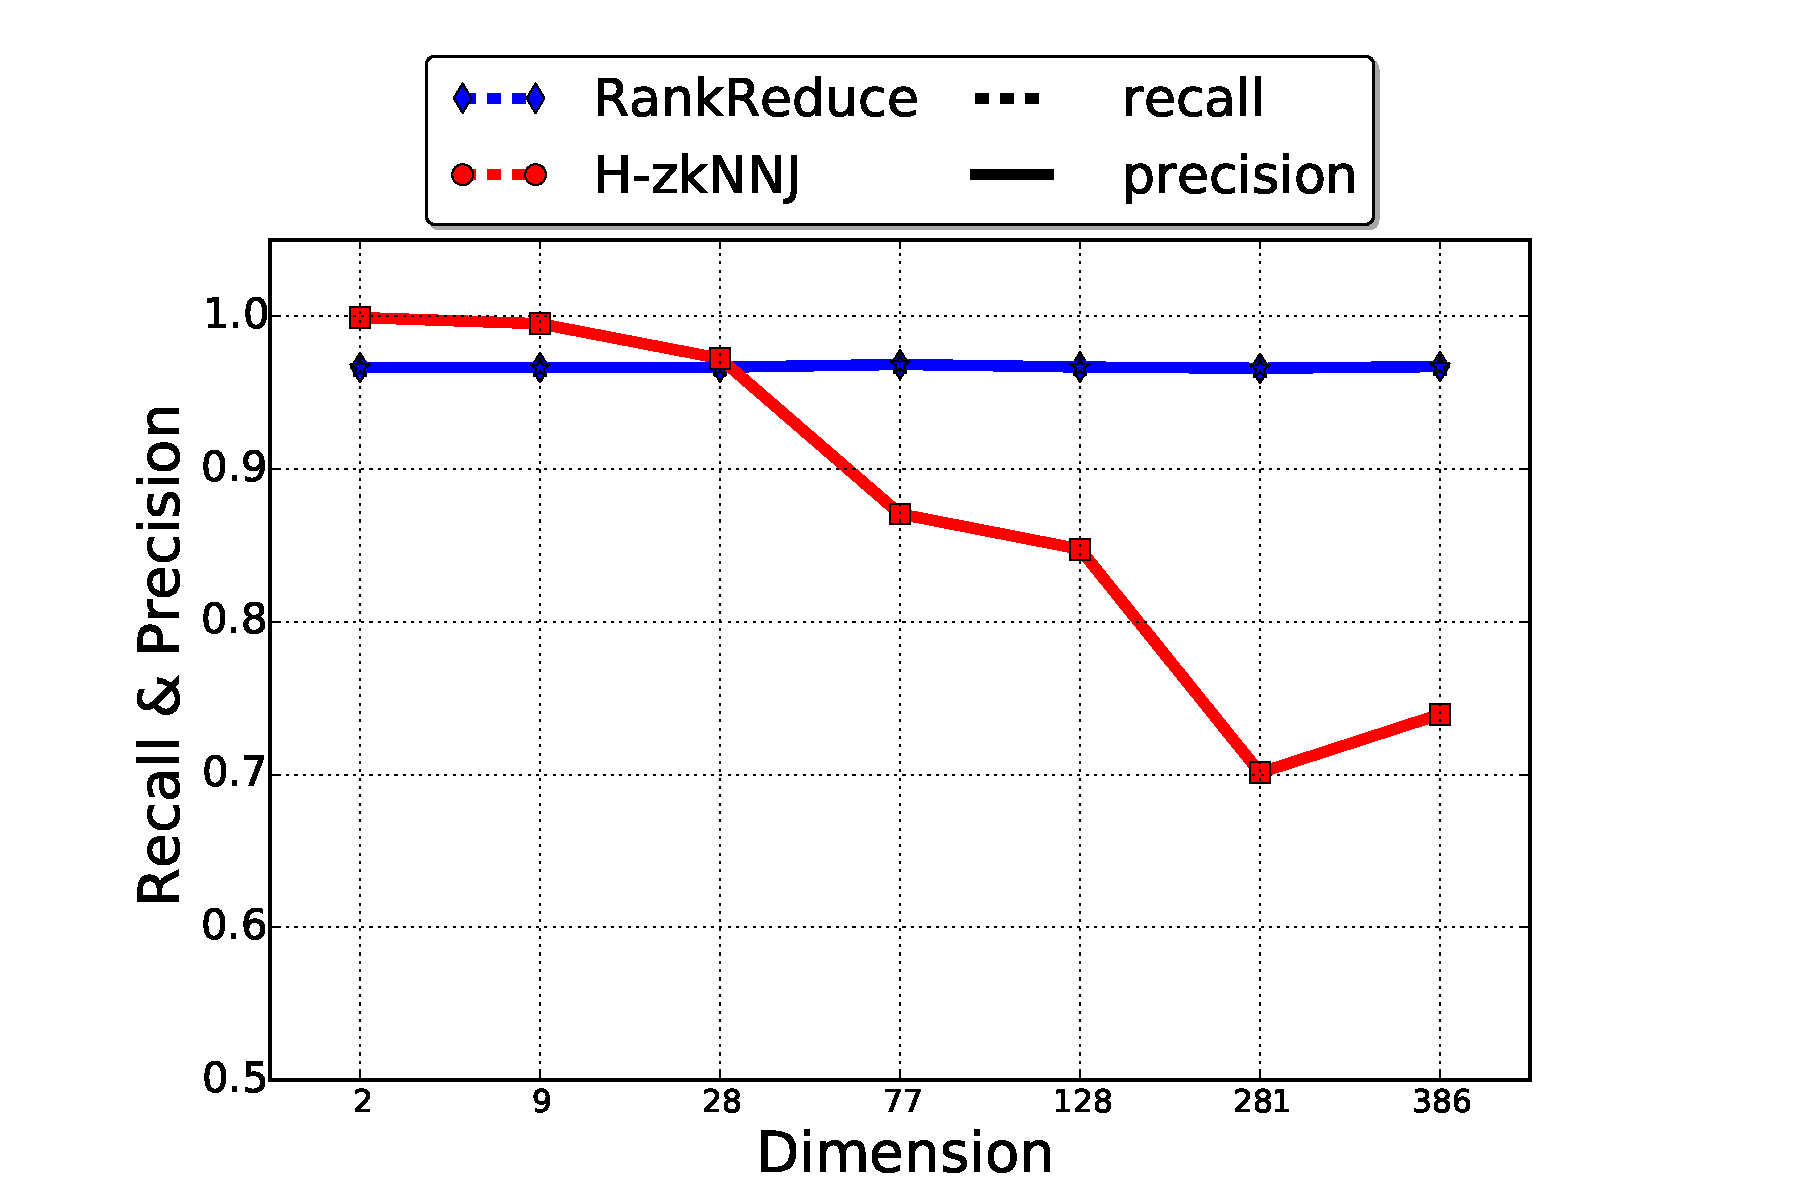
\includegraphics[width=1\textwidth]{img-perf/dim/randacc.pdf} 
	\caption{Recall and Precision}
	\label{fig:rand_acc}
\end{subfigure}%
\caption{Generated datasets of various dimensions}
\label{fig:dim_rand}
\end{figure*} 


Since \HBNLJ~relies on the dot product, it is not dataset dependent and its execution time increases
with the dimension as seen on Figures \ref{fig:dim_time} and \ref{fig:rand_time}. 

\VO~is heavily dependent on data distribution and on the choice of pivots to build clusters of 
equivalent size which improves parallelism. The comparison of execution times for the datasets 
\emph{128-sift} and \emph{281-blog} in Figure \ref{fig:dim_time} shows that, although the dimension
of data increases, the execution time is greatly reduced. Nonetheless, the clustering phase of the algorithm performs a 
lot of dot product operations which makes it dependent on the dimension, as can be seen in Figure \ref{fig:rand_time}. 

\Z~is an algorithm that depends on spatial dimension. Very efficient for low dimension, its 
execution time increases with the dimension (Figure \ref{fig:rand_time}). A closer 
analysis shows that all phases see their execution time increase. However, the overall time is 
dominated by the first phase (generation of shifted copies and partitioning) whose time complexity
sharply increases with dimension. Data distribution has 
an impact on the recall which gets much lower than the precision for some datasets (Figure~\ref{fig:dim_acc}).
With generated dataset (Figure~\ref{fig:rand_acc}), both recall and precision are identical and initially very high. 
However as dimension increases, the recall decreases because of the projection. 

Finally, \LSH~is both dependent on the dimension and distribution of data. Experiments with the real datasets have 
proved to be difficult because of the various parameters of the algorithm to obtain the requested number of 
neighbors without dramatically increasing the execution time (see discussion in Section~\ref{rankreduceanalysis}). 
Despite our efforts, the precision was very low for some datasets, in particular \emph{28-higgs}. 
Using the generated datasets, we see that its execution time increases with the dimension (Figure~\ref{fig:rand_time}) 
but its recall remains stable (Figure~\ref{fig:rand_acc}). 

\subsection{Practical Analysis}
In this section, we analyze the algorithms from a practical point of view, outlying their sensitivity to 
the dataset, the environment or some internal parameters.   
\subsubsection{H-BkNNJ}
%HBKNNJ
The main drawback of \HBK~is that only the Map phase is in parallel. In addition, the optimal parallelization 
is subtle to achieve because the optimal number of nodes to use is defined by  
$\frac{input\,size}{input\,split\,size}$. This algorithm is clearly not suitable for large datasets but because of its 
simplicity, it can, nonetheless, be used when the amount of data is small.  

\subsubsection{H-BNLJ}
In \HBNLJ, both the Map and Reduce phases are in parallel, but the optimal number of tasks is difficult to 
find. Given a number of partitions $n$, there will be $n^2$ tasks. Intuitively, one would choose a number of 
tasks that is a multiple of the number of processing 
units. The issue with this strategy is that the distribution of the partitions might be unbalanced.
Figure~\ref{fig:lb_hbnlj}
shows an experiment with $6$ partitions and $6^2=36$ tasks, each executed on a reducer. Some reducers will have more elements to process than others, 
slowing the computation.
\begin{figure}[!h]
\centering
   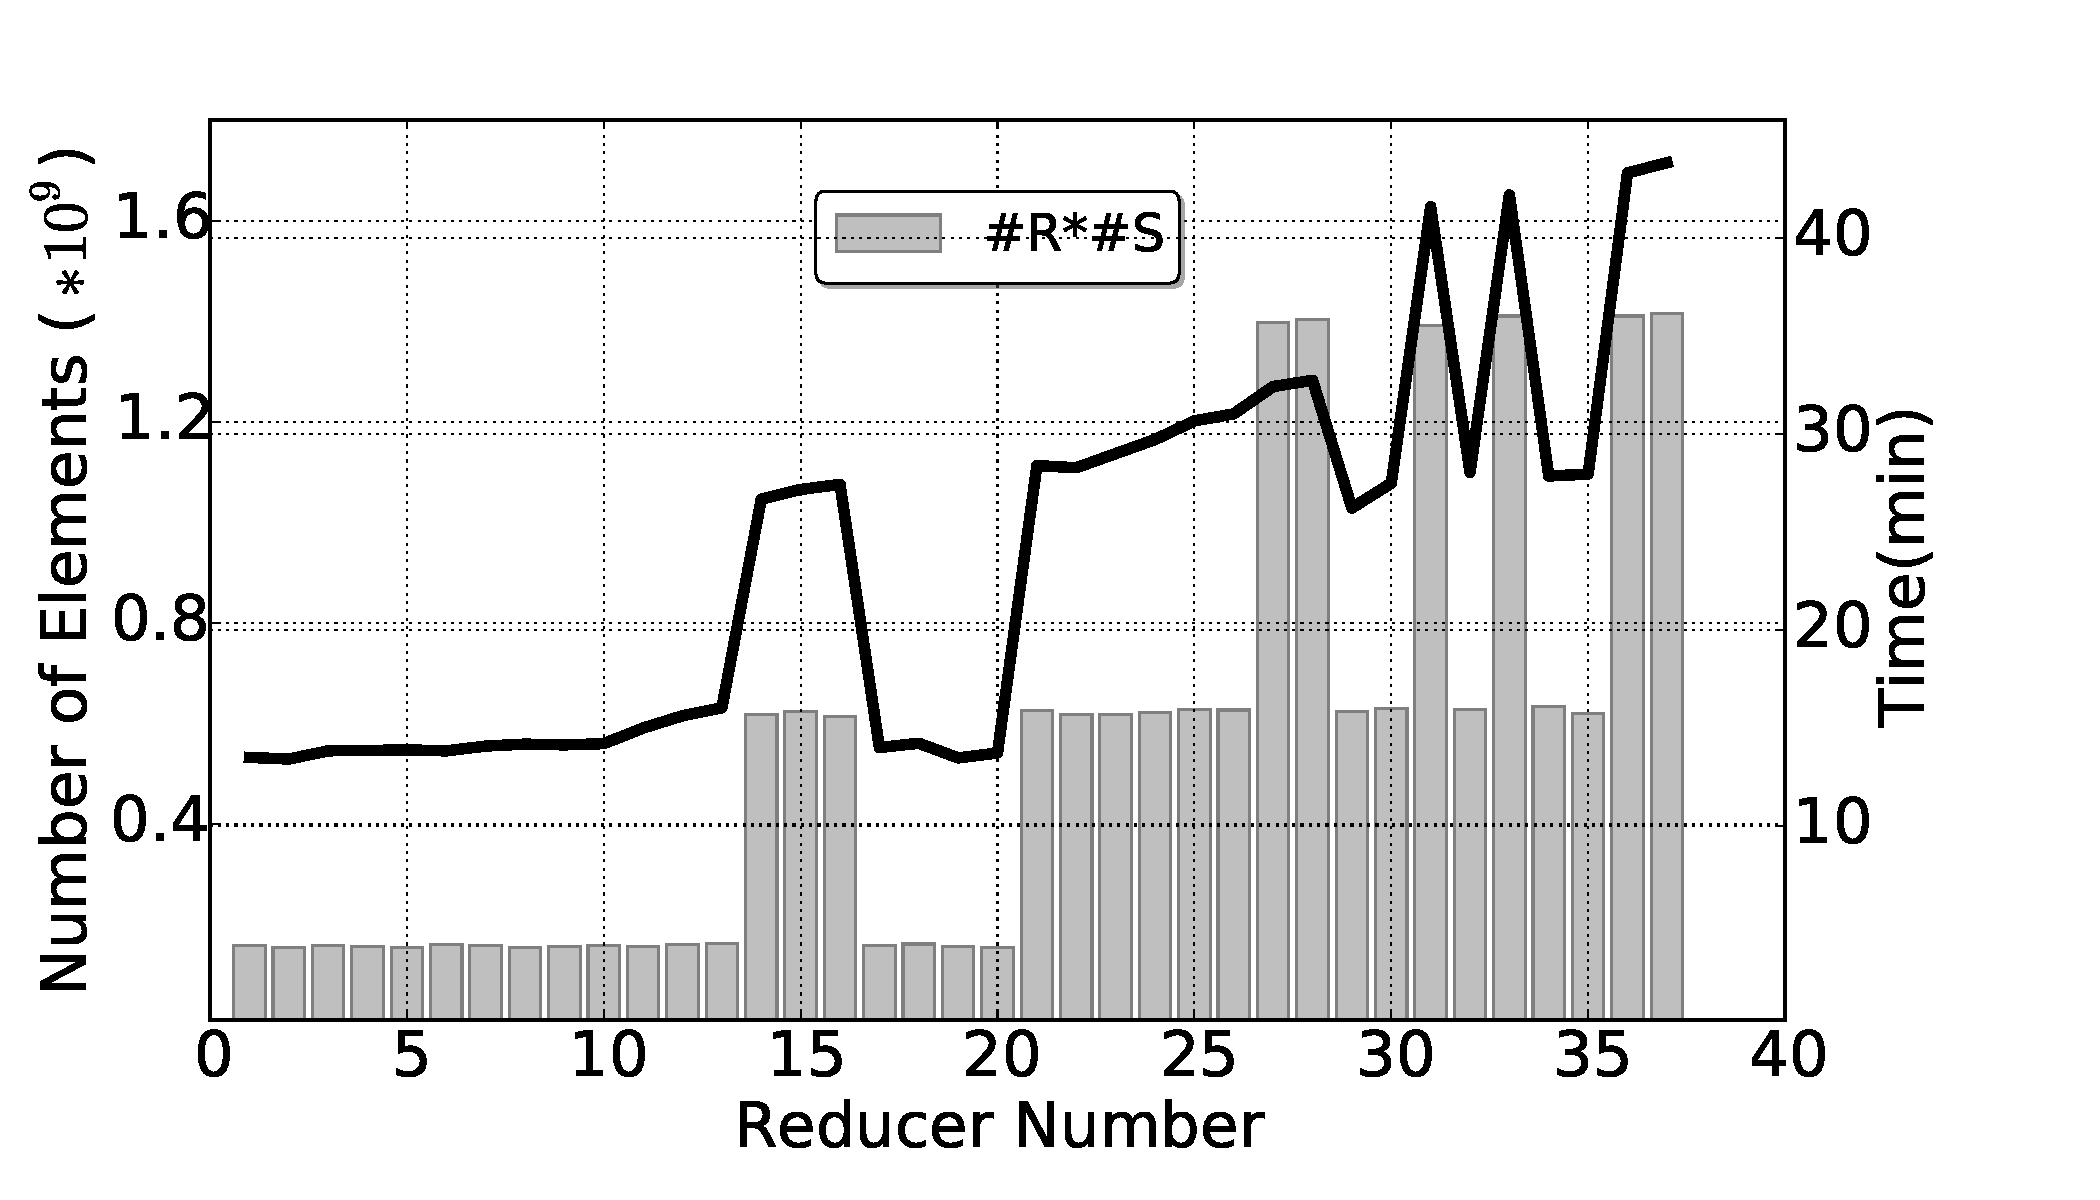
\includegraphics[width=0.4\textwidth]{img-perf/perso/loadbalancing/hbnlj.pdf}
   \caption{H-BNLJ, candidates job, $10^{5}$ records \label{fig:lb_hbnlj}, 6 partitions, Geo dataset}
\end{figure}%

Overall, the challenge with this algorithm is to find the optimal number of partitions for a given dataset. 

\subsubsection{PGBJ} 
A difficulty in \VO~comes from its sampling-based preprocessing techniques because it 
impacts the partitioning and thus the load balancing. This raises many challenges. First, how to choose
the pivots from the initial dataset. The three techniques proposed by the authors, farthest, k-means and 
random, lead to different pivots and different partitions and possibly different executions. We found that 
with  our datasets, both k-means and random techniques
gave the best performance. Second, the number of pivots is also important because
it will impact the number of partitions. A too small or too large number of pivots 
will decrease performance. Finally, another important parameter is the grouping strategy used 
(Section~\ref{pgbj_grouping}).
\begin{figure}[!h]
   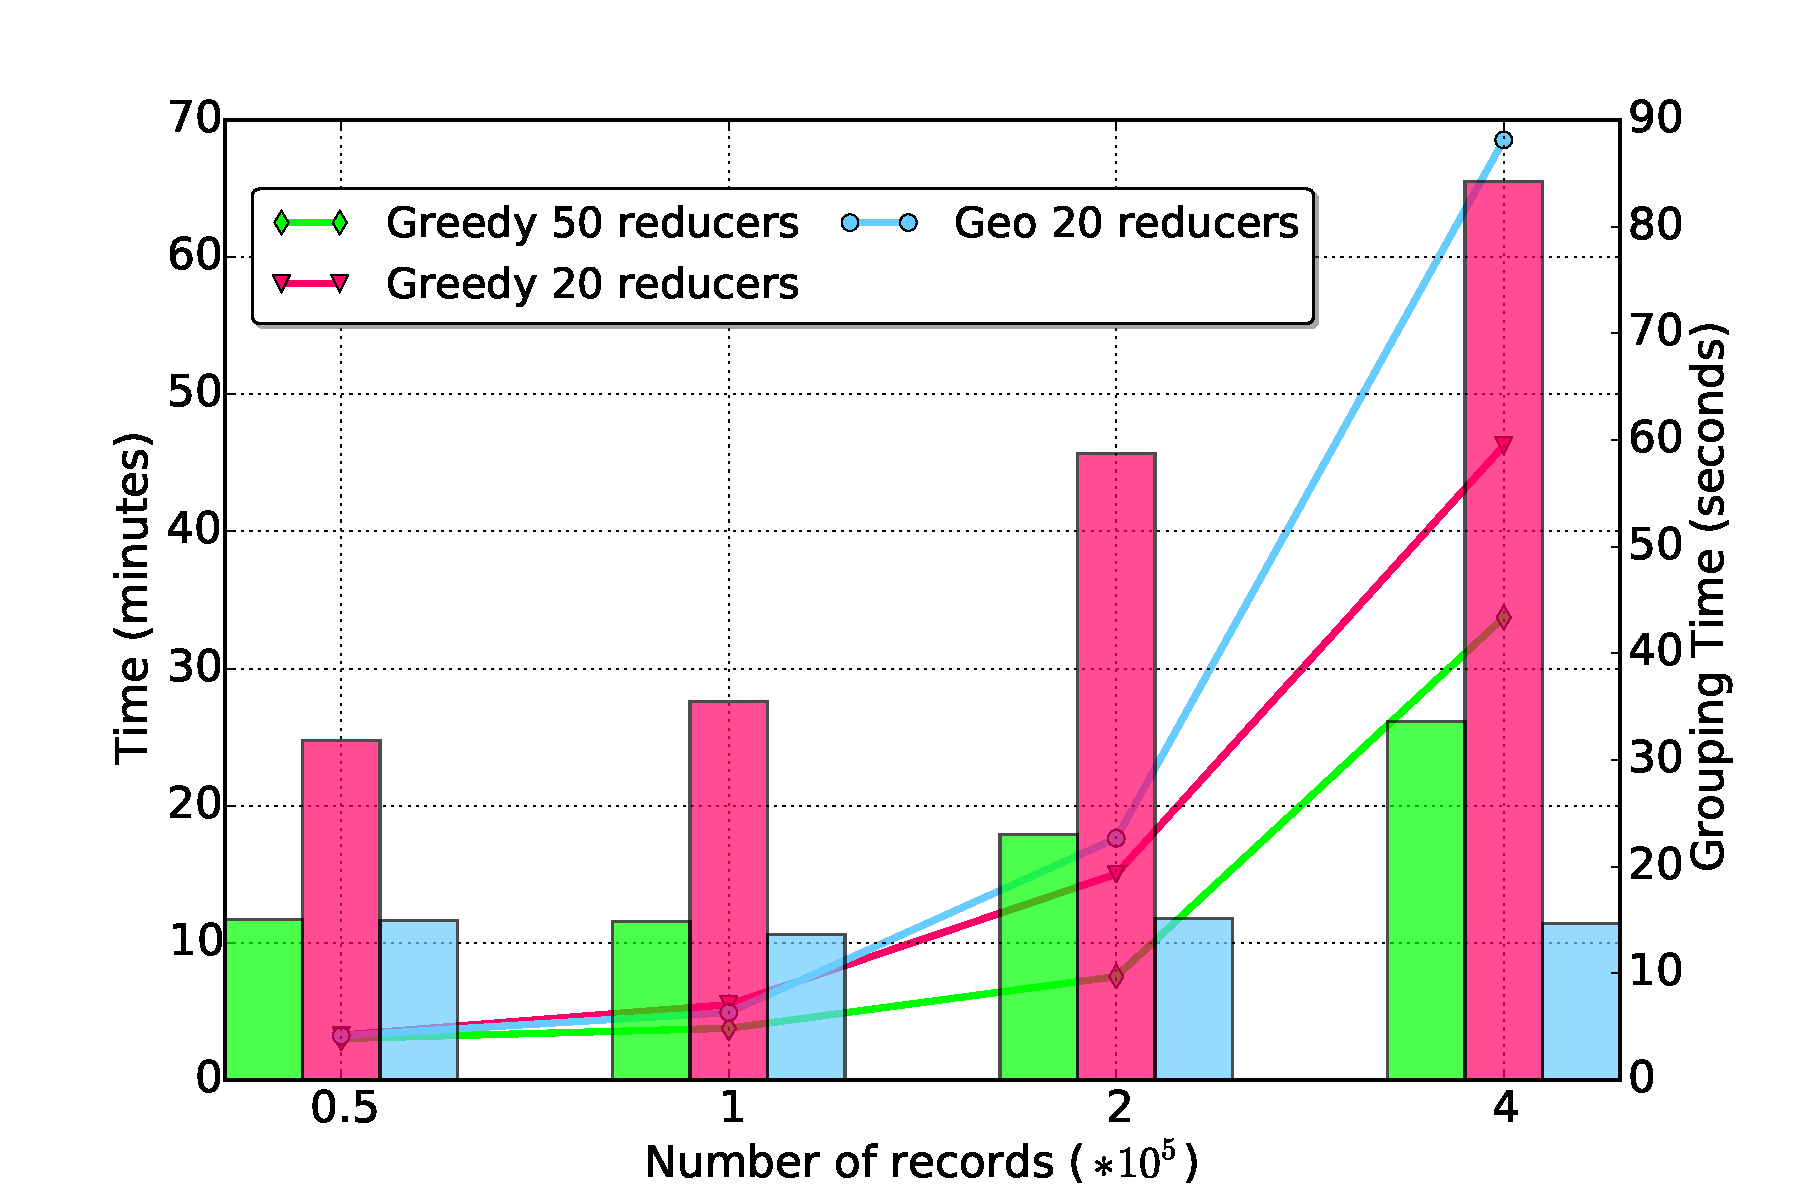
\includegraphics[width=0.5\textwidth]{img-perf/perso/pgbj/strategy.pdf} 
   \caption{PGBJ, overall time (lines) and Grouping time (bars)\label{fig:pgbj_strategy} with Geo dataset, 3000 pivots, 
   KMeans Sampling}         
\end{figure}
In Figure~\ref{fig:pgbj_strategy}, we can see that the greedy grouping technique has a higher grouping time 
(bars) than the geo grouping technique. 
However, the global computing time (line) using this technique is shorter thanks to the good load balancing. This
is illustrated by Figure~\ref{fig:pgbj_balancing} which shows the distribution of elements processed
by reducers when using geo grouping (\ref{fig:geo_20r}) or greedy grouping (\ref{fig:greedy_20r}).
                  
\begin{figure}[h]
\centering
		\begin{subfigure}[b]{0.25\textwidth}
                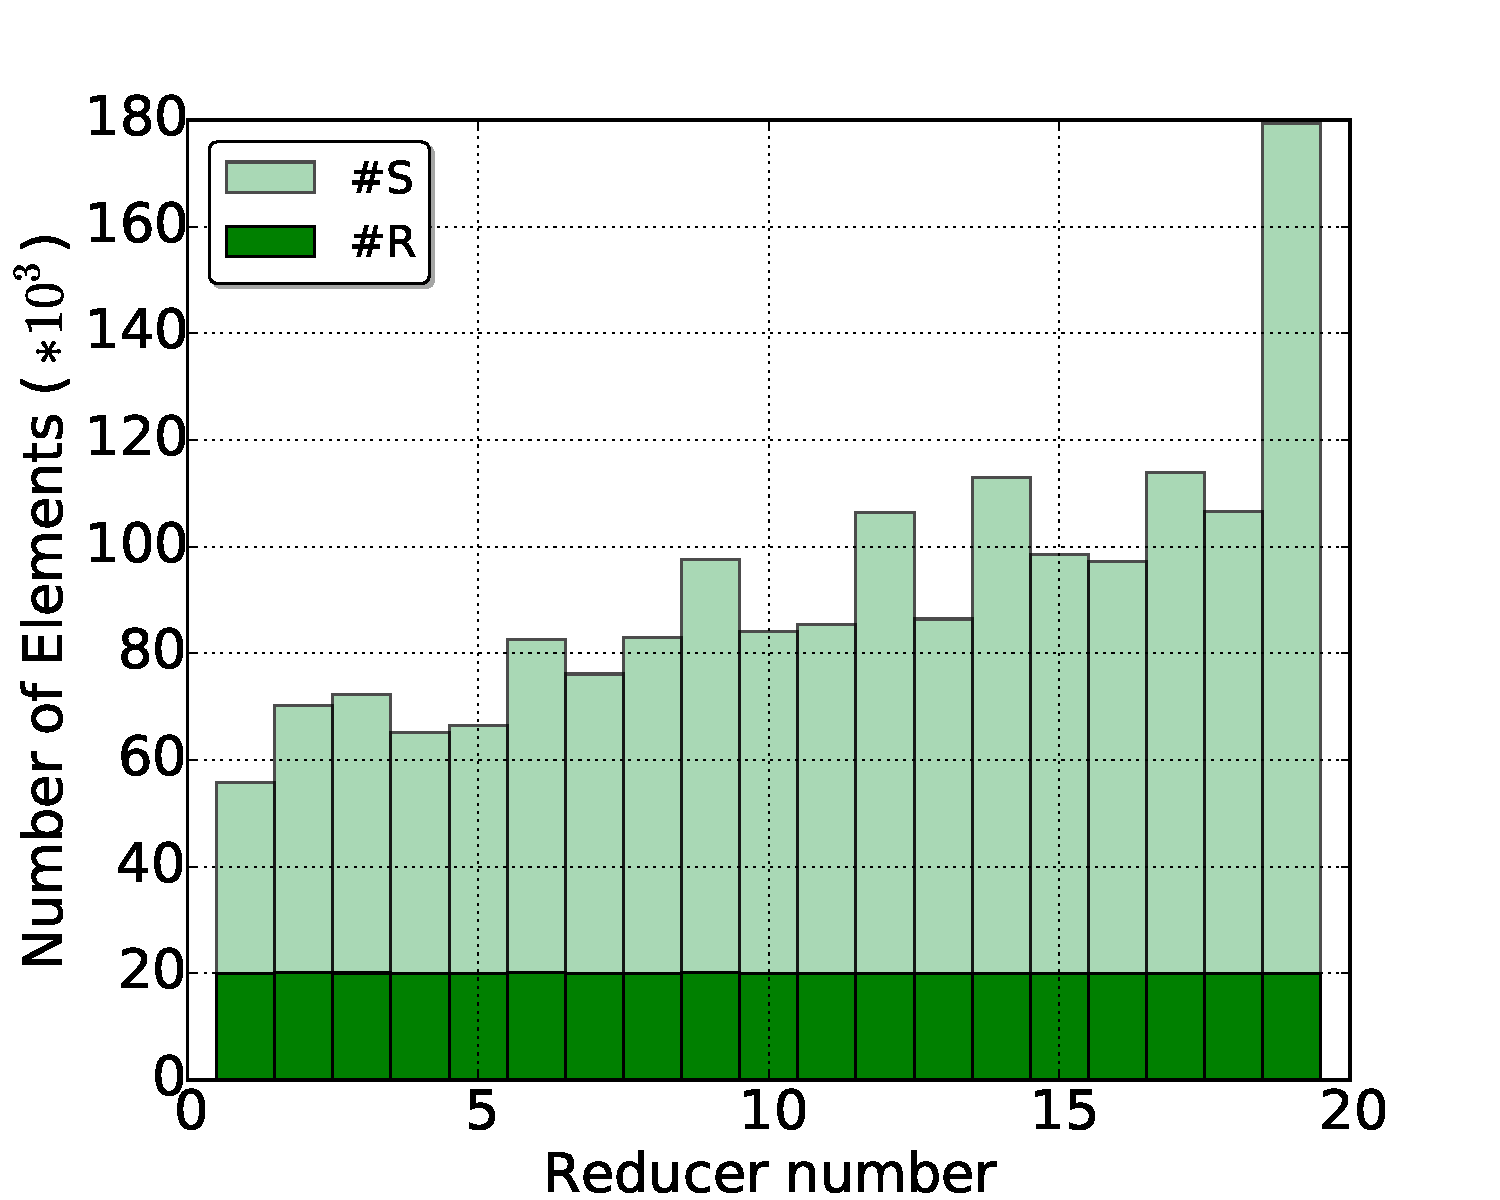
\includegraphics[width=\textwidth]{img-perf/perso/pgbj/geo_20r_400.pdf}
                \caption{Geo\label{fig:geo_20r}}
                
        \end{subfigure}%
        \begin{subfigure}[b]{0.25\textwidth}
                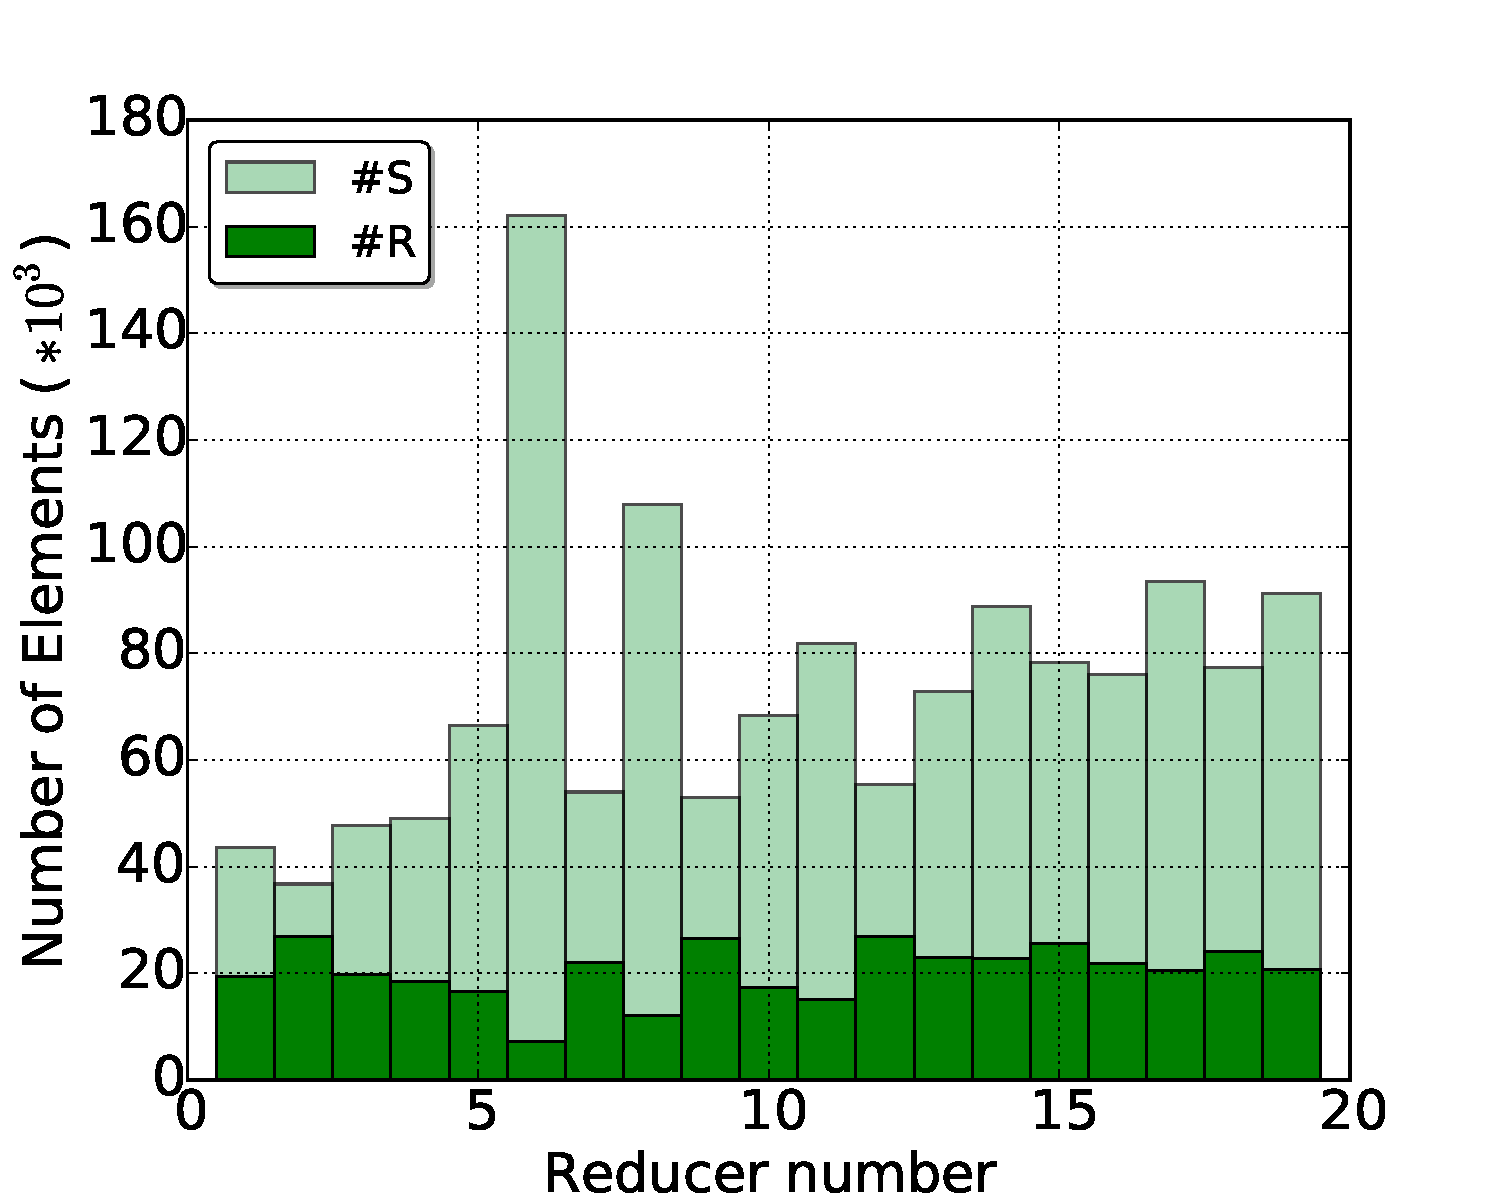
\includegraphics[width=\textwidth]{img-perf/perso/pgbj/greedy_20r_400.pdf}
                \caption{Greedy\label{fig:greedy_20r}}
                
        \end{subfigure}%
        \caption{PGBJ, load balancing \label{fig:pgbj_balancing} with 20 reducers}
\end{figure}                
 
\subsubsection{H-zkNNJ}\label{z-value}
In \Z, the $z$-value transformation leads to information loss. The recall of this algorithm is influenced
by  the nature, the dimension and the size of the input data.
More specifically, this algorithm becomes biased if the distance between initial data is very scattered, and 
the more input data or the higher the dimension, the more difficult it is to draw the space filling curve. To 
improve the recall, the authors propose to create duplicates in the original dataset by shifting data. 
This greatly increases the amount of data to process and has a significant impact on the execution time.

\begin{table*}[ht]
 	\begin{center}\renewcommand{\arraystretch}{1.2}
 		\begin{tabular}{|c|c|c|c|}
 			\hline
 			\textbf{Algorithm}  & \textbf{Advantage}  &  \textbf{Shortcoming}   & \textbf{Typical Usecase} \\
 			 \hline
 			\textbf{H-BkNNJ} 	& 
 				\begin{tabular}[c]{@{}c@{}}
 					Trivial to implement  
 				\end{tabular} & 
 				\begin{tabular}[c]{@{}c@{}}
 					1. Breaks very quickly \\ 
 					2. Optimal parallelism difficult\\ 
 					to achieve a priori
 				\end{tabular} &
 				\begin{tabular}[c]{@{}c@{}}
 			    	Any tiny and low dimension dataset\\
 			    	($\sim$ 25000 records)
 			    \end{tabular} \\ \hline
 			\textbf{H-BNLJ}     &
 				\begin{tabular}[c]{@{}c@{}}
 				 	Easy to implement
 				\end{tabular} & 
 				\begin{tabular}[c]{@{}c@{}}
 				 	1. Slow\\
 				 	2. Very large communication overhead 
 				\end{tabular} & 
 				\begin{tabular}[c]{@{}c@{}}
 				 	Any small/medium dataset\\
 				 	($\sim$ 100000 records)
 				\end{tabular} \\ \hline
 			\textbf{PGBJ}       & 
	 			\begin{tabular}[c]{@{}c@{}}
 				   	1. Exact solution\\ 
 				   	2. Lowest disk usage\\ 
 			       	3. No impact on communication\\
 			       	overhead with the increase of $k$
	 			\end{tabular}        & 
	 			\begin{tabular}[c]{@{}c@{}}
	 				1. Cannot finish in reasonable time\\ 
	 				for large dataset\\ 
	 				2. Poor performance for high\\
	 				dimension data\\
	 				3. Large communication overhead\\
	 				4. Performance highly depends on\\ 
	 				the quality of a priori chosen pivots
	 			\end{tabular} & 
 				\begin{tabular}[c]{@{}c@{}}
 					1. Medium/large dataset for\\
 					low/medium dimension\\
 					2. Exact results
 				\end{tabular} \\ \hline
 			\textbf{H-zkNNJ}    &
	 			\begin{tabular}[c]{@{}c@{}}
	 			    1. Fast\\ 
	 			    2. Does not require a priori parameter\\ 
	 			    tuning \\ 
	 			    3. More precise for large k \\ 
	 			    4. Always give the right number of $k$	 	
	 	        \end{tabular} & 
	 	        \begin{tabular}[c]{@{}c@{}}
	 	        	1. High disk usage\\ 
	 	        	2. Slow for large dimension \\ 
	 	        	3. Very high space requirement ratio \\ 
	 	        	for small values of $k$
 				\end{tabular} & 
 				\begin{tabular}[c]{@{}c@{}}
 					1. Large dataset of small dimension\\
 					2. High values of $k$\\
 			        3. Approximate results
 				\end{tabular} \\ \hline
 			\textbf{RankReduce} & 
 			\begin{tabular}[c]{@{}c@{}}
 				1. Fast\\ 
 				2. Low footprint on disk usage
 			\end{tabular} & 
 			\begin{tabular}[c]{@{}c@{}}
 				1. Fine parameter tuning required with\\ 
 				experimental set up \\
 				2. Multiple hash functions needed for\\
 				acceptable recall \\
 				3. Different quality metrics to consider\\
 				(recall + precision)
 		   \end{tabular}                                           
 			& \begin{tabular}[c]{@{}c@{}}
 				1. Large dataset of any dimension \\
 				2. Approximate results \\
 				3. Room for parameter tuning
 			\end{tabular} \\ \hline
 		\end{tabular}
 		\caption{Summary table for each algorithm in practice}\label{summary_practice}  
 	\end{center}
 \end{table*}

\subsubsection{RankReduce}\label{rankreduceanalysis}
\LSH, with the addition of a third job, can have the best performance of all, provided that it is started with the 
optimal parameters.
The most important ones are $W$, the size of each bucket, $L$, the number of hash families and $M$, the number 
of hash functions in each family. Since they are dependent on the dataset, experiments are 
needed to precisely tune them. In \cite{Dong:2008:MLP:1458082.1458172_full}, the authors suggests this can be achieved 
with a sample dataset and a theoretical model. 
The first important metric to consider is the number of candidates available in each bucket. Indeed, with some 
poorly chosen parameter values, it is possible to have less than $k$ elements in each bucket, making it impossible to 
have enough elements at the end of the computation (there are less than $k$ neighbors in the result). On the opposite, 
having too many candidates in each bucket will increase too much the execution time. 
To illustrate the complexity of the parameter tuning operation, we have run experiments on the Geo and SURF datasets. 
First, Figure~\ref{fig:lsh_tunning_geo} shows that, for the Geo dataset, increasing $W$ improves the recall and the 
precision at the expense of the execution time, up to an optimal before decreasing. This can be explained by looking
at the number of buckets for a given $W$. As $W$ increases, each bucket contains more elements and thus their number 
decreases. As a consequence, the probability to have the correct $k$ neighbors inside a bucket increases, which 
improves the recall. However, the computational load of each bucket also increases.

 
\begin{figure}[!h]
 \centering
          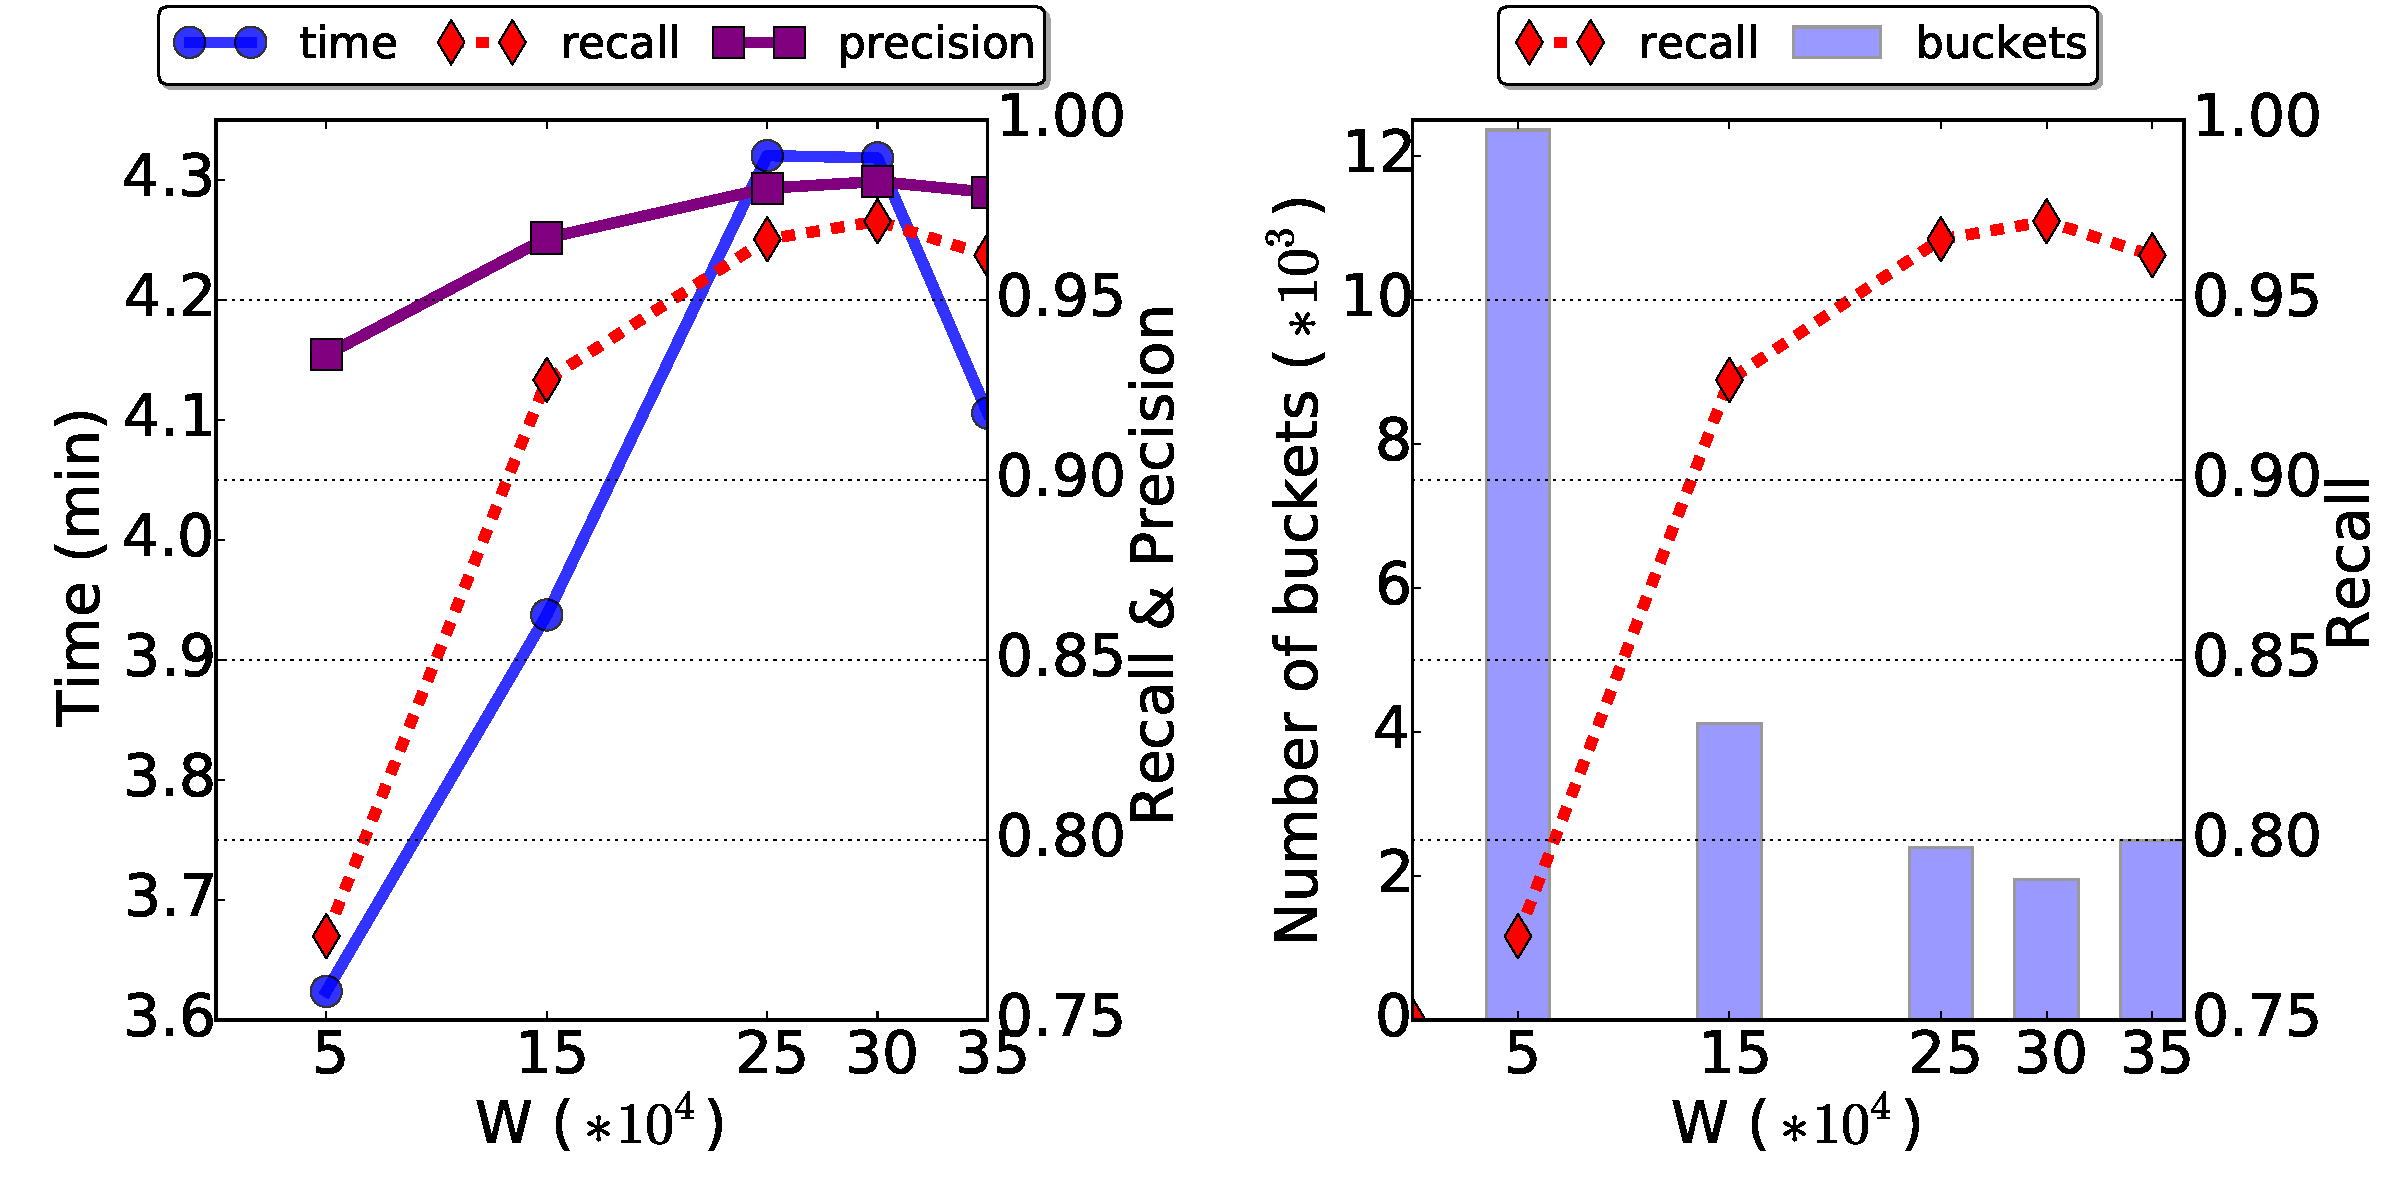
\includegraphics[width=0.5\textwidth]{img-perf/perso/lsh/params_geo_time.pdf} 
         \caption{LSH tuning, Geo dataset, 40k records,  20 nodes}
                \label{fig:lsh_tunning_geo}
\end{figure}
\begin{figure}[!h]
         \centering
       % \begin{subfigure}[b]{0.25\textwidth}
                 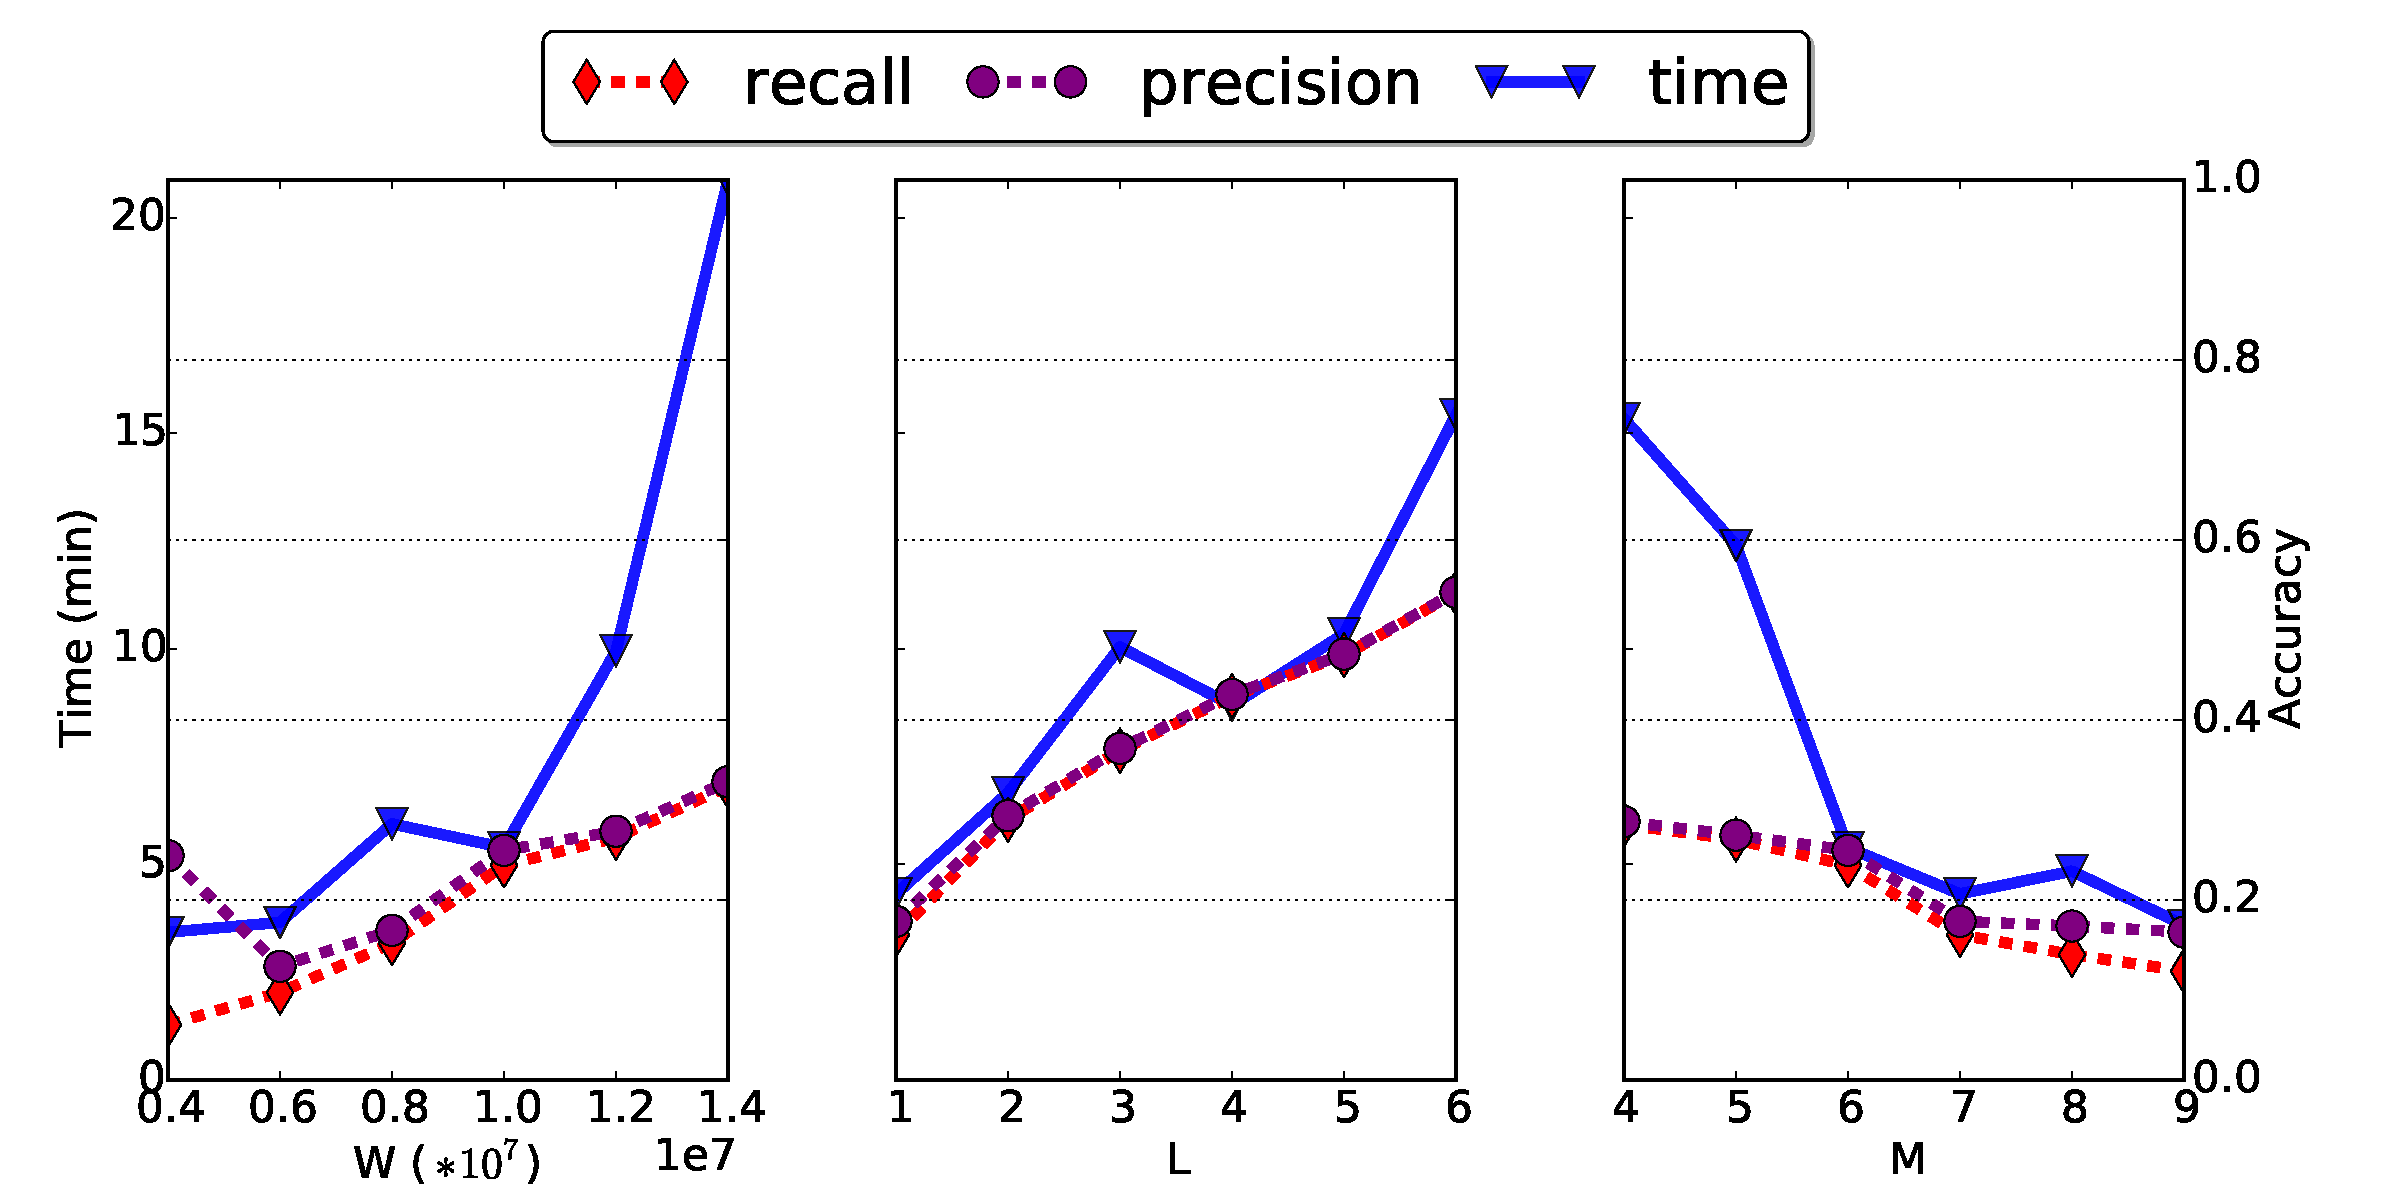
\includegraphics[width=0.5\textwidth]{img-perf/perso/lsh/params_surf.pdf} 
                %\caption{lsh tunning surf}
        %\end{subfigure}
         \caption{LSH tuning, SURF dataset, 40k records, 20 nodes}\label{fig:lsh_tunning_surf}
\end{figure}

A similar pattern can be observed with the SURF dataset (Figure~\ref{fig:lsh_tunning_surf}, left), where 
increasing $W$ improves the recall (from 5\% to 35\%) and the precision (from 22\% to 35\%). Increasing 
the number of families $L$ greatly improves both the precision and recall. However, increasing $M$, the
number of hash functions, decreases the number of collisions, reducing execution time but also the recall and 
precision. Overall, finding the optimal parameters for the LSH part is complex and has to be done for every dataset

After finishing all the experiments, we found that the execution time of all algorithms mostly follows the 
theoretical analysis presented in Section~\ref{sec:analysis}. However, as expected, the computationally intensive
part, which could not be expressed analytically, has proved to be very sensitive to a lot of different factors.
The dataset itself, through its dimension and the data distribution, but also the parameters of some of the 
pre-processing steps. The magnitude of this sensitivity and its impact on metrics such as recall and precision
could not have been inferred without thorough experiments. 


\subsection{Lessons Learned}

The first aspect is related to load balance. \HBNLJ~actually cannot guarantee load balancing, because of the random 
method it uses to split data. For \VO, Greedy grouping gives a better load balance than Geo grouping, at 
the cost of an increased duration of the grouping phase. At 
the same time, our experiments also confirm that \Z~and \LSH, which use size based 
partitioning strategies, have a very good load balance, with a very small deviation of the completion time of each 
task. %\TODO{3s out of how long? we need to put a \% ---done}

Regarding disk usage, generally speaking, \VO~has the lowest disk space requirement, while \Z~has the largest for small
$k$ values. However, for large $k$, the space requirement of all algorithms becomes similar. 
%\TODO{better word, comparable en francais}.

The communication overhead of \VO~is very sensitive to the choice of pivots. 

The data are another important aspect affecting the performance of the algorithms. As expected, all the 
algorithms' performance decreases as the dimension of data increases. However, what exceeded the prediction of the 
theoretical analysis is that the dimension is really a curse for \VO~. Because of the cost of computing distances in 
the pre-processing phase, its performance becomes really poor, sometimes worse than \HBNLJ. \Z~also suffers from the 
dimension, which decreases its recall. However, the major impact comes from the distribution of data. 

In addition, the overall performance is also sensitive to some specific parameters, especially for \LSH. Its 
performance depends a lot on some parameter tuning, which requires extensive experiments.

Based on the experimental results, we summarize the advantages, disadvantages and suitable usage scenarios for each 
algorithm, in Table~\ref{summary_practice}.


 